Many measurements of standard model properties or searches for new physics beyond the standard model performed within the CMS experiment rely on events with jets in the final state. Hence, a good understanding of jet properties is of major importance and a crucial ingredient for such kind of analyses. One of such properties is the jet transverse-momentum resolution, as introduced in Sec.~\ref{subsec:jets_response}. \\
Many new physics searches are carried out based on final states containing missing transverse momentum and several jets. Here, QCD multijet events can fake the signature of possible new physics events and constitute a background process, since a mismeasurement of the jet momenta due to the limited detector resolution or the decay of heavy flavour quarks leads to a momentum imbalance in the event and consequently to measurable missing energy. The knowledge of the jet resolution is thus a keypoint in the prediction of such background contributions, as discussed later in Chap.~\ref{chap:RA2}. \\
In this chapter, an analysis is presented in which the jet-\pt resolution in data and in simulated events is derived. The method is based on momentum conservation in the transverse plane of dijet events and offers the possibility to cover a large phase space in \pt and $\eta$. A similar approach was already used in previous studies at $\sqrt{s}=7$\tev~\cite{1748-0221-6-11-P11002, thesis:Schroeder} while a complementary approach utilizes $\gamma +\rm{jet}$ events~\cite{CMS-AN-2010-141, CMS-AN-2011-004, CMS-AN-2013-179}. The measurement shown here is based on collision data corresponding to an integrated luminosity of $19.7$~\fbinv recorded at $\sqrt{s}=8$\tev in 2012. Parts of this chapter are taken from~\cite{bib:AN2013-416}, having been written by the author.   
\section{Components of the Jet Response}
\label{sec:jer_response}
\begin{figure}[!tp]
  \centering
  \begin{tabular}{c}
                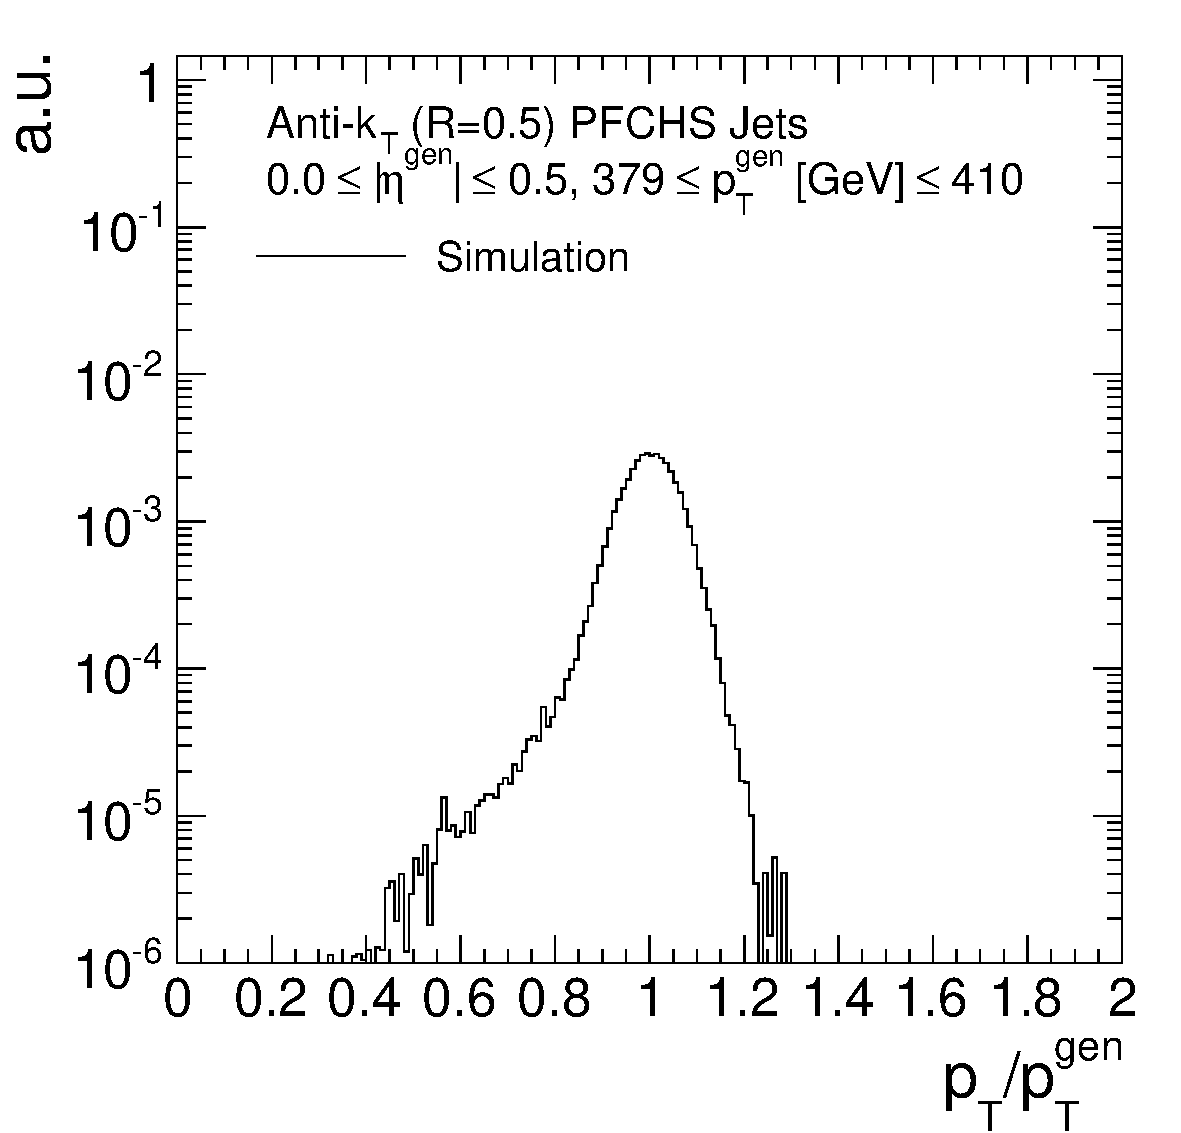
\includegraphics[width=0.49\textwidth]{figures/TruthResponse_example_test.pdf}
  \end{tabular}
  \caption{Jet response distribution for one example $|\eta^\mathrm{gen}|$ and $\pt^\mathrm{gen}$ interval derived from simulation.}
  \label{fig:response}
\end{figure}
As introduced in Sec.~\ref{subsec:jets_response}, the relation of the transverse momentum of a jet at detector level to the momentum of the corresponding particle-level jet is expressed by the jet response. In simulated events, the transverse momentum of the particle-level jet is known and corresponds to the \pt of the generated jet, which is clustered from all stable particles after hadronisation and decay, including neutrinos. Thus, the \textit{MC-truth response} can be determined as
\begin{equation}
\mathcal{R} = \frac{\pt}{\pt^{\mathrm{gen}}} \; .
\end{equation}
 In Fig.~\ref{fig:response}, an example for a jet response distribution derived from simulation is shown. It is obtained from a QCD multijet sample generated with $\textsc{Pythia6}$ tune Z2~\cite{Chatrchyan:2011id} using the CTEQ6L1 PDF set~\cite{Pumplin:2002vw} and processed with the full detector simulation. For the calculation of the truth response, the two generated jets in the event with highest transverse momentum are selected. The event is rejected, if one of these two generator jets does not have a corresponding reconstructed jet within a distance of $\Delta R < 0.25$. Otherwise, the response is calculated in intervals of $\pt^\mathrm{gen}$ and $|\eta^\mathrm{gen}|$. This is done since a dependence on the momentum and the respective detector region is expected, as discussed in Sec.~\ref{subsec:jets_response}. The calculation of the jet response is performed after applying the jet energy corrections discussed in Sec.~\ref{subsec:jets_calib} to the detector-level jet momenta, so that the mean of the response distribution is located at one. \\
Apparently, the jet response distribution consists of two components: the Gaussian-shaped core around the mean referred to as jet resolution and non-Gaussian components referred to as tails. \\
The core of the response is mainly caused by the intrinsic resolution of the various sub-detector components and the precision of the PF algorithm. Since the jet momenta obtained from the PF constituents are based on tracking- as well as calorimeter-based measurements, the jet resolution is closely connected to the evolution of the tracking and calorimeter resolution with \pt. In the tracking system, the intrinsic resolution is mainly caused by the uncertainty on the track curvature. This is limited by multiple scattering at low \pt and by the finite hit-position resolution at high \pt. In total, the track-\pt resolution degrades for increasing transverse momentum. However, the evolution of the resolution in the calorimeters behaves the other way round and improves with increasing momentum. At low momenta, the calorimeter resolution is mainly dominated by electronic noise and pileup while at medium momenta the resolution is driven by fluctuations of the shower development. At high energies, however, the resolution is eventually limited by calorimeter miscalibration and non-uniformities. Furthermore, the response also depends on the jet flavour. Typically, quark jets consist of less and harder particles than gluon jets and thus have a different detector response due to the non-linearity of the calorimeters.  \\
The response tails are caused by severe jet-momentum mismeasurements. These can for instance be due to detector effects. Shower leakage can occur, if not the whole shower is deposited in the calorimeters. Due to the limited length of the calorimeters, some particles might even cross the whole apparatus (\textit{punch-through}). Also malfunctioning detector components can lead to high or low reponse tails by creating artifical signals. Beyond that, also physics processes lead to response tails. For instance, the lower response tails get populated by semi-leptonic decays of heavy-flavour quarks. These contain neutrinos that carry a certain amount of the momentum and leave the detector unnoticed resulting in an overall reduced response. 

\section{Basic Concept of the Dijet Asymmetry Method}
\label{sec:jer_method}
As introduced in Sec.~\ref{subsec:jets_response} and~\ref{sec:jer_response}, the jet transverse momentum resolution corresponds to the width of the Gaussian-shaped core part of the jet response. In simulated events, the particle-level jet momenta are given by the generator-level jet momenta. In data events, however, no such equivalent is present so that the jet resolution is not accessible directly. \\
One possibility to measure the resolution of the jet transverse momenta in data as well as in simulated events is to utilize the dijet asymmetry $\mathrm{A}$. For events with at least two jets it is defined as
\begin{equation}
\label{eq:asymmdef}
  \mathrm{A} = \frac{p_\mathrm{T,1} - p_\mathrm{T,2}}{p_\mathrm{T,1} + p_\mathrm{T,2}} \, .
 \end{equation}
 In this equation $p_\mathrm{T,1}$ and $p_\mathrm{T,2}$ correspond to the randomly ordered transverse momenta of the two leading jets. \\
 Neglecting tails, the asymmetry is approximately normally distributed, with mean $= 0$, and the standard deviation is given as
 \begin{equation}
 \label{eq:asymm_first}
  {\sigma_{\mathrm{A}}} = \left\lvert \frac{\partial \mathrm{A}}{\partial p_\mathrm{T,1}} \right\rvert \cdot \sigma(p_\mathrm{T,1}) \oplus  \left\lvert \frac{\partial \mathrm{A}}{\partial p_\mathrm{T,2}} \right\rvert \cdot \sigma(p_\mathrm{T,2}) \; .
 \end{equation}
 In an ideal dijet topology, the two jets are exactly balanced at particle level. If they belong in addition to the same $\eta$ region, then $\langle p_\mathrm{T,1} \rangle = \langle p_\mathrm{T,2} \rangle = \langle \pt \rangle$ and $\sigma (p_\mathrm{T,1}) = \sigma (p_\mathrm{T,2}) = \sigma (\pt)$. This allows the simplification of Eq.~\ref{eq:asymm_first} and provides the following important relation between the width of the asymmetry $\sigma_\mathrm{A}$ and the jet-\pt resolution $\sigma (\pt)$
 \begin{equation}
 \label{eq:asymm}
  \frac{\sigma (p_\mathrm{T})}{\langle p_\mathrm{T} \rangle} = \sqrt{2} \cdot \sigma_\mathrm{A} \; .
 \end{equation}
This relationship was already used at the Tevatron experiments~\cite{oai:arXiv.org:hep-ex/0012046, JetsD0}, the ATLAS experiment~\cite{Aad:2012ag} or in previous CMS analyses~\cite{1748-0221-6-11-P11002, thesis:Schroeder} to measure the jet resolution from dijet events. 

\section{Application to Realistic Collision Events}
\label{sec:jer_application}
The measurement of the jet transverse momentum resolution in collision events is based on Eq.~\ref{eq:asymm}. As discussed in Sec.~\ref{subsec:jets_response}, the resolution is a function of \pt and $\eta$. In order to account for this dependence, the asymmetry has to be recorded in intervals of pseudorapidity and a measure for the transverse momentum scale of the event, as \eg the \pt of the leading jet, as well. However, the jet-\pt spectrum is affected by migration effects such that momentum measures based on single jets are not preferable. Due to the limited jet resolution, a particular interval of reconstructed jet momenta is populated not only by jets whose particle-level jet momentum belongs to that bin. In case of a steeply falling spectrum, as it is the case for jet momenta, more jets with low $\pt^\mathrm{gen}$ migrate into a specific interval than jets with high $\pt^\mathrm{gen}$. Consequently, the measured response is systematically higher and the measured relative response is biased towards the object with worse resolution. In order to reduce this resolution bias in the analysis, the measurement is performed in intervals of the average momentum of the two leading jets in the event
\begin{equation}
\ptave = \frac{1}{2}(p_\mathrm{T.1} + p_\mathrm{T,2}) \; .
\end{equation}
Beyond that, the ideal dijet topology with exactly two jets that are perfectly balanced, is interferred with additional effects in realistic collision events. Very often, further jet activity is occuring as momentum of the hard scattering process is transferred to soft particles or jets arising from initial or final state radiation leading to momentum imbalance in the dijet system. This additional jet activity can be described by the variable $\alpha$ which is defined as the ratio of the transverse momentum of the third jet to the average momentum according to
 \begin{equation}
\label{eq:alpha}
\alpha = \frac{p_\mathrm{T,3}}{\pt^\mathrm{ave}} \, .
\end{equation}
The presence of jets beyond the third is neglected in the parametrization of the additional activity in the event, as these have consecutively declining momentum due to the strongly decreasing jet production cross section versus jet-\pt~\cite{CMS-PAS-QCD-11-004}. The presence of additional jets and the thereby introduced imbalance leads to a broadening of the observed asymmetry distribution. This effect is also illustrated later in Sec.~\ref{subsec:jer_sel_cuts}. In order to determine the intrinsic resolution from such events, the measured resolution has to be corrected for this effect. \\
A further source of momentum differences between the particle-level and the detector-level jet leading to an overall momentum imbalance in an event is arising from out-of-cone showering effects. Typically, some particles might be too soft to be included in the clustered jet. Furthermore, additional contributions from the underlying event might be wrongly asscociated to a jet. In general, such effects have to be considered in the resolution measurement as well. \\
The actual procedure how to determine and apply the required corrections is discussed in Sec.~\ref{sec:jer_corrections}.

\section{Samples and Event Selection}
\label{sec:jer_selection}
%In this section the data samples used for the analysis are specified (Section~\ref{subsec:jer_samples_and_trigger}). Furthermore, selection criteria applied on data and simulated events in order to select events with a dijet-like topology are discussed (Section~\ref{subsec:jer_sel_cuts}). 

\subsection{Datasets and Triggers}
\label{subsec:jer_samples_and_trigger}
\begin{table}[!tp]
\centering
\caption{Trigger paths with \ptave thresholds at which the trigger efficiency reaches the $99\%$ efficiency plateau. Thresholds are given for PFCHS jets.}
\label{tab:trigger}
 \makebox[\linewidth]{
\begin{tabular}{lccc}
\multicolumn{4}{c}{} \\
\toprule
 Trigger & & \ptave threshold [GeV] \\
\midrule
 HltDiPFJetAve40 & & 62 \\
 & & & \\
 HltDiPFJetAve80 & & 107 \\
 & & & \\
 HltDiPFJetAve140 & & 175 \\
 & & & \\
 HltDiPFJetAve200 & & 242 \\
 & & & \\
 HltDiPFJetAve260 & & 310 \\
 & & & \\
 HltDiPFJetAve320 & & 379 \\
 & & & \\
 HltDiPFJetAve400 & & 467 \\
\bottomrule
\end{tabular}}
\end{table}  
In this analysis, multijet events from \pp collisions are considered which have been recorded in 2012 with the CMS detector at $\sqrt{s}=8$\tev. From these data, only those are considered in which all subdetectors have been reliably operating. The collected data sample used in this analysis corresponds to an integrated luminosity of $19.7$~\fbinv with an uncertainty of $2.5\%$ (syst.)  $\pm \; 0.5\%$ (stat.)~\cite{CMS-PAS-LUM-13-001}. \\
Multijet events are pre-selected by a set of triggers based on the average transverse momentum of the two leading jets in the event. In order to obtain a good coverage of the \ptave spectrum, different trigger paths are combined. Since they have different minimum $\pt^\mathrm{ave}$ thresholds, a broad range in \ptave is considered. In Tab.~\ref{tab:trigger} the different trigger paths used for this analysis are listed and the particular offline $\pt^\mathrm{ave}$ value for which the respective trigger reaches $99\%$ of the efficiency plateau is given~\cite{DRathjens}.%website:HamburgCalib}).
However, the low \ptave triggers have been operated with prescale factors applied in order to keep the data rate sufficiently low. In fact, only the trigger with the highest \ptave threshold has been employed without the usage of prescale factors. \\
The simulated QCD sample that is used in the analysis is generated with \pythia, as discussed in Section~\ref{sec:jer_response}. Since the cross-section of the process has been scaled by $\hat{p}_\mathrm{T}^{\,4.5}$, with the scale parameter $\hat{p}_\mathrm{T}$ describing the momentum transfer in the hard process, the sample is reweighted with the inverse in order to regain the physical spectrum.  

\subsection{Selection Criteria}
\label{subsec:jer_sel_cuts}
The physics objects used in the analysis are reconstructed with the PF algorithm including charged-hadron subtraction, as described in Sec.~\ref{sec:pf_algo}. Jets are clustered with the anti-$k_\mathrm{T}$ algorithm using a distance parameter of $R=0.5$. They are calibrated in data and simulation following the procedure introduced in Sec.~\ref{subsec:jets_calib}.  \\
The event selection described in the following is designed to enhance the dataset with events featuring a typical dijet-like event topology. This is characterized by two hard jets being back-to-back in $\phi$ direction. Thus, only events with at least two jets are considered for the analysis. These two leading jets in the event have to fulfill loose jet identification (\textit{jet-id}) criteria which remove fake jets originating from detector noise while maintaining an efficiency of more than $99\%$ for real jets~\cite{CMS-PAS-JME-09-008, CMS-PAS-JME-10-003}. In order to mitigate effects from pileup, only jets with $\pt > 10$\gev are considered for the analysis. As discussed in Sec.~\ref{sec:jer_application}, events with a topology of exactly two high-\pt jets and no further jet activity are very rare in realistic collisions. Thus, events with additional jets have to be selected to perform the measurement. Since very soft jets do not necessarily have to belong to the hard interaction, but could arise from pileup, it is required that each event has a third jet passing the \pt threshold of 10\gev while fulfilling also loose jet identification criteria. Furthermore, the additional jet activity has to be restricted to a maximal amount in order to maintain a dijet-like structure of the event. Thus, a maximum threshold for the relative third jet momentum of 
\begin{equation*}
\alpha < 0.25 
\end{equation*}
is introduced. In order to enrich the sample with events close to the ideal dijet topology, in which two jets point into opposite directions in the transverse plane, the two leading jets have to fulfill 
\begin{equation}
|\Delta \phi| > 2.7 \; \mathrm{with} \; \Delta \phi = \Delta \phi(\vec{p}_\mathrm{T,1}, \vec{p}_\mathrm{T,2}) \, .
\end{equation}  
The selection criteria described above are applied to data and simulation in an identical manner. However, a further adjustment is necessary for the simulated sample. Typically, the simulation is performed before the actual data taking takes place. Thus, it is unknown which specific pileup conditions will be present in data and the simulation is performed with an estimated pileup scenario. Hence, it is necessary to adjust the simulation to the actual pileup scenario in data. This is done by reweighting the simulated events to match the mean pileup distribution in data. However, the pileup distribution in data differs for each individual trigger. Since the instantaneous luminosity changed throughout the data taking in 2012, the pileup conditions changed accordingly. As stated above, the trigger paths utilized in this analysis have been mainly operated with prescale factors applied, in order to meet the changing running conditions over time. 
\begin{figure}[!t]
  \centering
  \begin{tabular}{cc}
                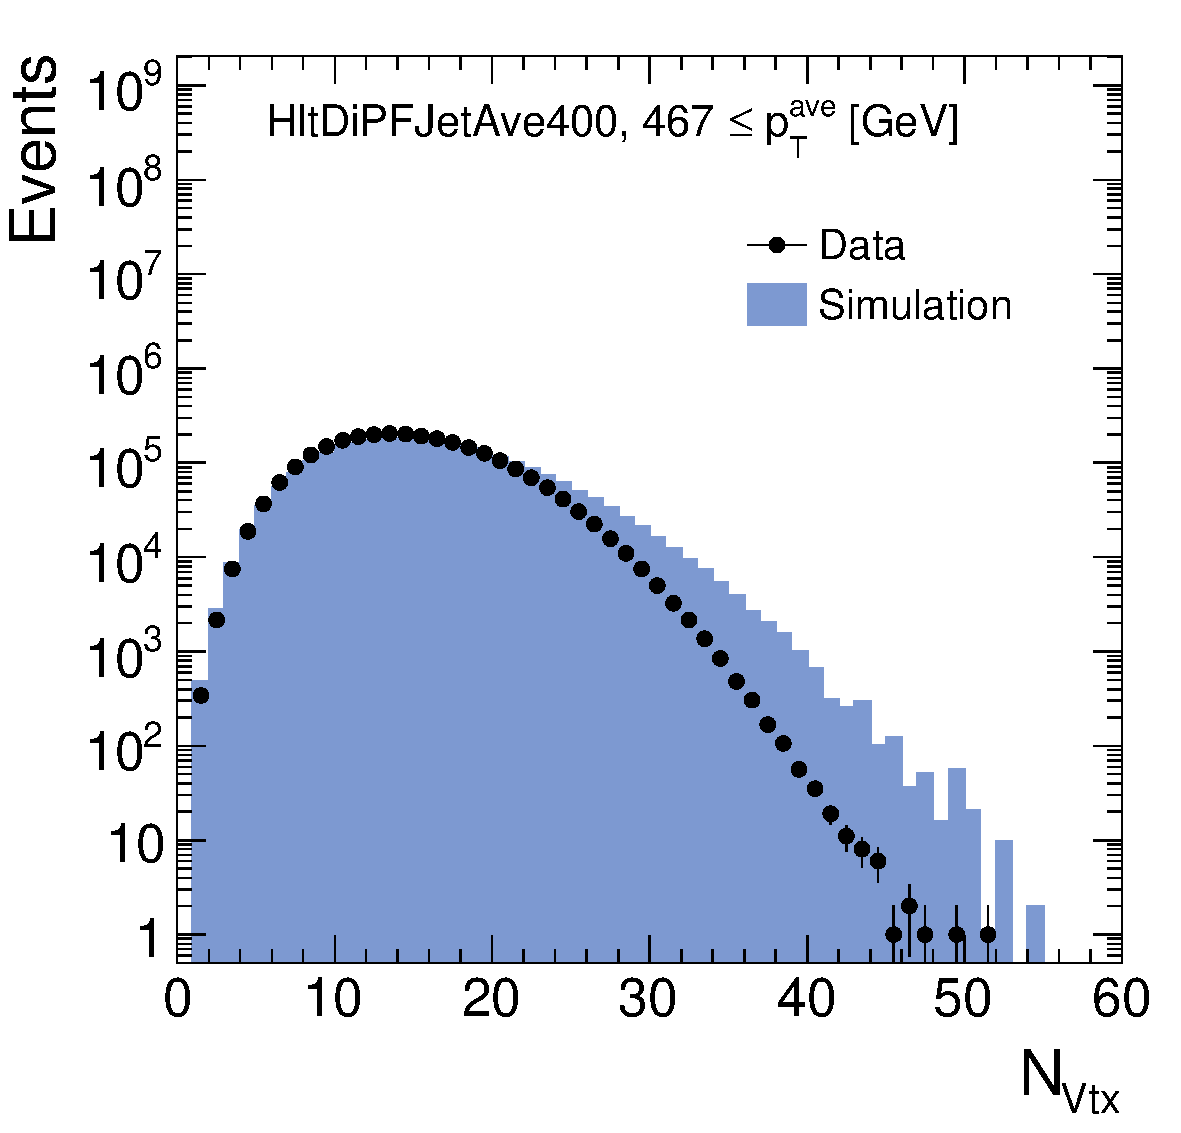
\includegraphics[width=0.49\textwidth]{figures/NVtx_HltDiPFJetAve400_AfterTriggerSelection.pdf} &
                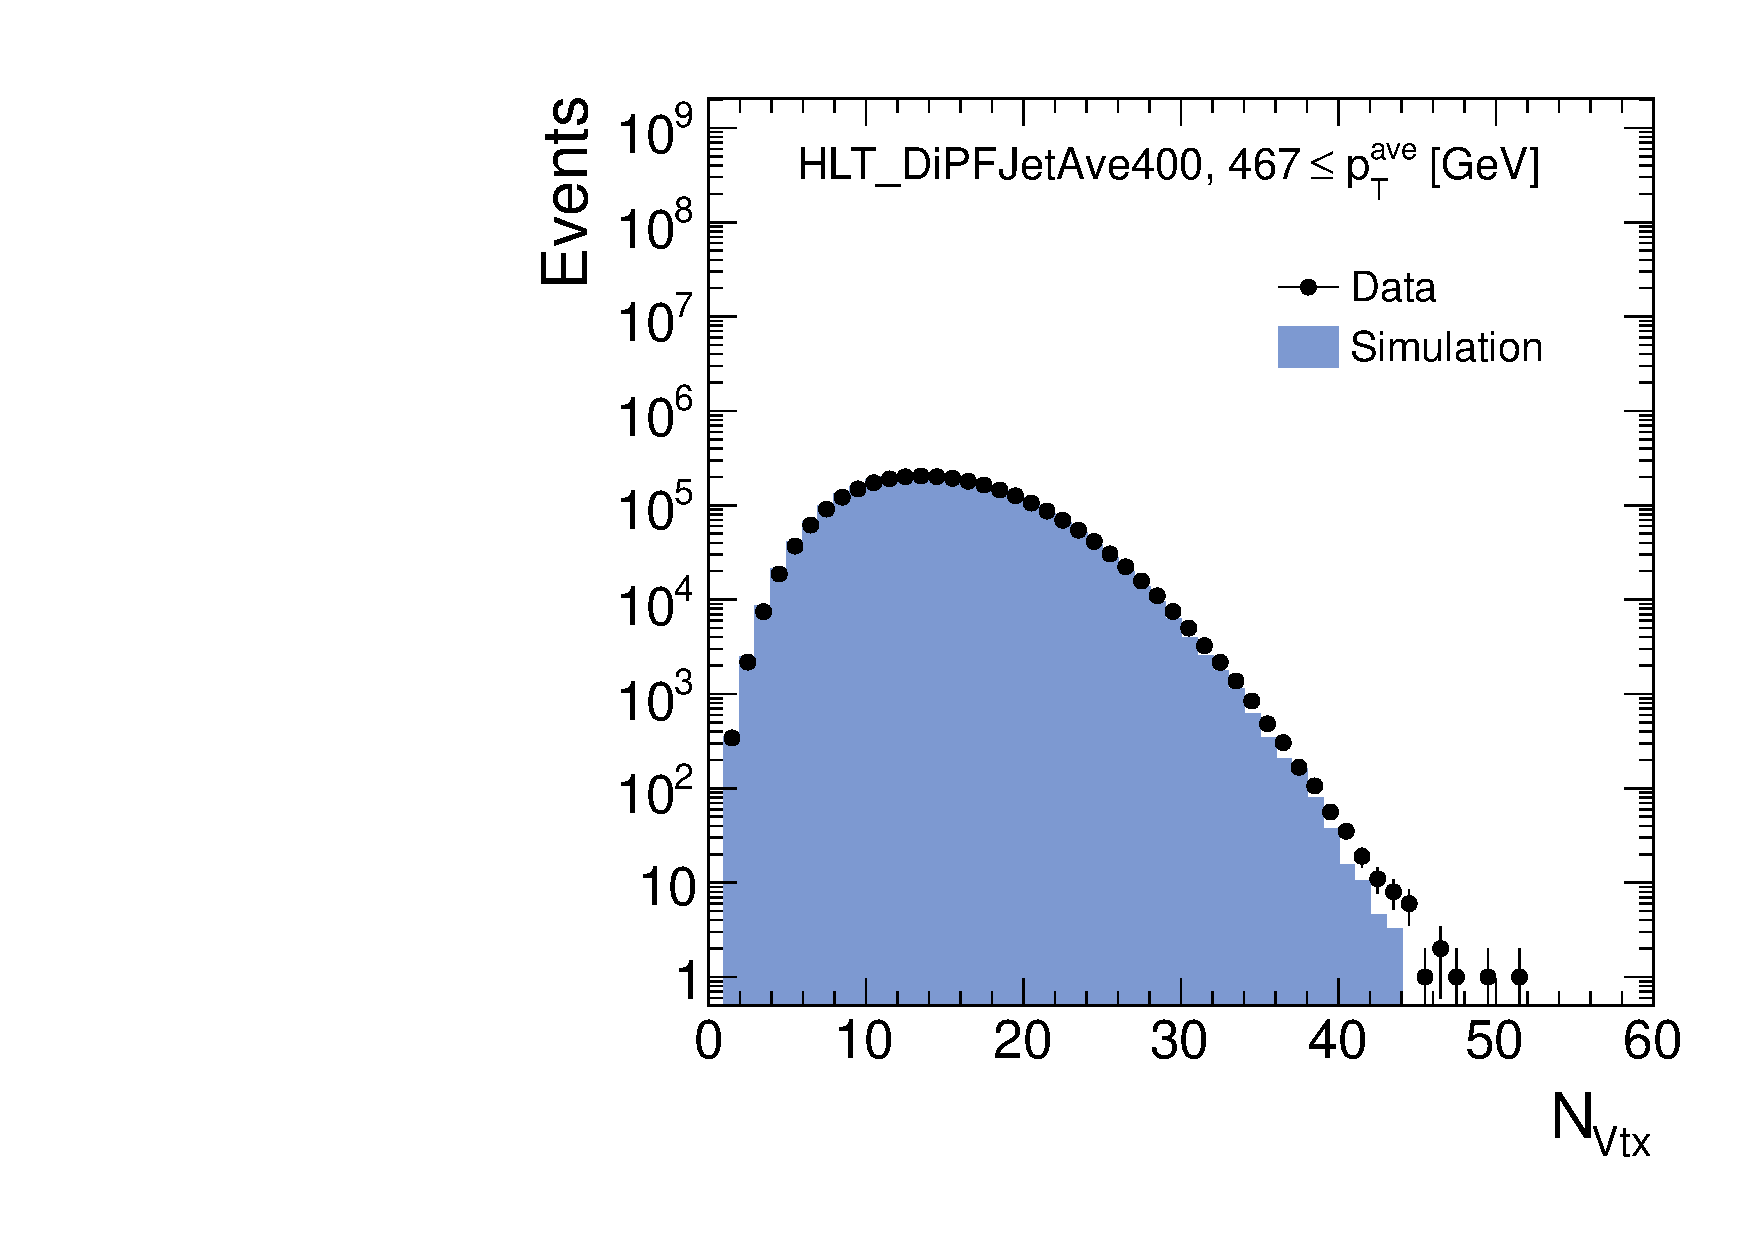
\includegraphics[width=0.49\textwidth]{figures/NVtx_HltDiPFJetAve400_AfterPUReweighting.pdf}
  \end{tabular}
  \caption{Distribution of number of primary vertices in data (black dots) and simulation (blue histogram) before (\textit{left}) and after (\textit{right}) reweighting of the pileup scenario in simulation for trigger path HltDiPFJetAve400.}
  \label{fig:pu_reweight}
\end{figure}
Thus, each trigger path collected different amounts of data and consequently also the pileup distribution differs per trigger. Hence, the reweighting of the pileup scheme is done for each trigger path individually. Depending on the offline \ptave, a simulated event can be unambigously assigned to the corresponding trigger path, which is fully efficient for that particular \pt range, and reweighted to that particular pileup scenario. Since the number of primary vertices in the event is a measure for the pileup activity, the success of the reweighting procedure can be checked by comparing the distribution of the number of primary vertices in data and simulation before and after reweighting, respectively. Such a comparison is shown in Fig.~\ref{fig:pu_reweight} for the trigger path with the highest \ptave threshold. The primary vertex distributions show a good agreement after the application of the reweighting procedure, especially in the bulk of the distribution. Corresponding distributions of other trigger paths used in the analysis are shown in App.~\ref{app:jer_pu_reweight}. The pileup weight is considered as a multiplicative factor for each simulated event. \\
In order to account for the dependence of the resolution on the transverse momentum and $\eta$, the asymmetry distributions are derived for various intervals of $|\eta|$ and $\pt^\mathrm{ave}$. These are summarized in Tab.~\ref{tab:binning}. The \ptave intervals are chosen in correspondence to the \ptave values for which the different triggers become fully efficienct. If a trigger path provides enough statistical precision, the interval is separated into two. This definition of \ptave intervals ensures that all events in one \ptave interval are selected by the same trigger. The same interval boundaries are chosen for simulated events as well. The $|\eta|$ intervals are chosen to reflect the actual detector geometry. The most central part of the detector is covered by $ 0.0 < |\eta| < 0.5$, $0.5 < |\eta| < 1.1$ while the transition region, where the ECAL ends, is separated into an individiual bin $ 2.8 < |\eta| < 3.2$. The forward detector is covered by one large bin $|\eta| = 3.2 - 5.0$ mainly due to the small number of available events. In order to allow the application of Eq.~\ref{eq:asymm} for the determination of the resolution, both leading jets are required to belong to the same $|\eta|$ interval $\Delta |\eta|$
\begin{equation}
 \Delta |\eta|_{\mathrm{jet},1} = \Delta |\eta|_{\mathrm{jet},2}
\end{equation}
\begin{table}[!t]
\centering
\caption{Overview of the $|\eta|$ and $\pt^\mathrm{ave}$ interval boundaries used for the resolution measurement.}
\label{tab:binning}
\makebox[\linewidth]{
\begin{tabular}{c}
\multicolumn{1}{c}{} \\
\toprule
 $|\eta|$ \\
 0.0, 0.5, 1.1, 1.7, 2.3, 2.8, 3.2, 5.0 \\
\midrule
$\pt^\mathrm{ave}$ [GeV] \\
62, 107, 175, 205, 242, 270, 310, \\
335, 379, 410, 467, 600, 1000, 2000 \\
\bottomrule
\end{tabular}}
\end{table} 
To account for the $\alpha$-dependence of the measured asymmetry distributions, the \ptave and $|\eta|$ intervals are further subdivided in various $\alpha$ intervals. These are chosen such that each $\alpha$ interval ranges from $\alpha = 0.0$ to a particular upper boundary $\alpha_\mathrm{max}$. The respective upper boundaries of the $\alpha_\mathrm{max}$ intervals are $0.1, 0.125, 0.15, 0.175, 0.2, 0.225, 0.25$. This inclusive definition of the $\alpha$ intervals implicates that one specific event might be assigned to more than one $\alpha$ bin. \\
The resulting inclusive $\pt^\mathrm{ave}$ spectrum after applying the the described selection is shown for data and simulationin Fig.~\ref{fig:ptave_spec}. The \pt spectra of the first three leading jets are shown as well. The number of simulated events in each trigger $\pt^\mathrm{ave}$ interval is normalized to the respective integral in data. It is visible that the shapes of the spectra in data and simulation agree well. Furthermore, the effect of the pre-scales applied to the low-\ptave-threshold triggers is nicely visible resulting in the sawtooth-shaped \ptave-spectrum.  
\begin{figure}[!tp]
  \centering
  \begin{tabular}{cc}
                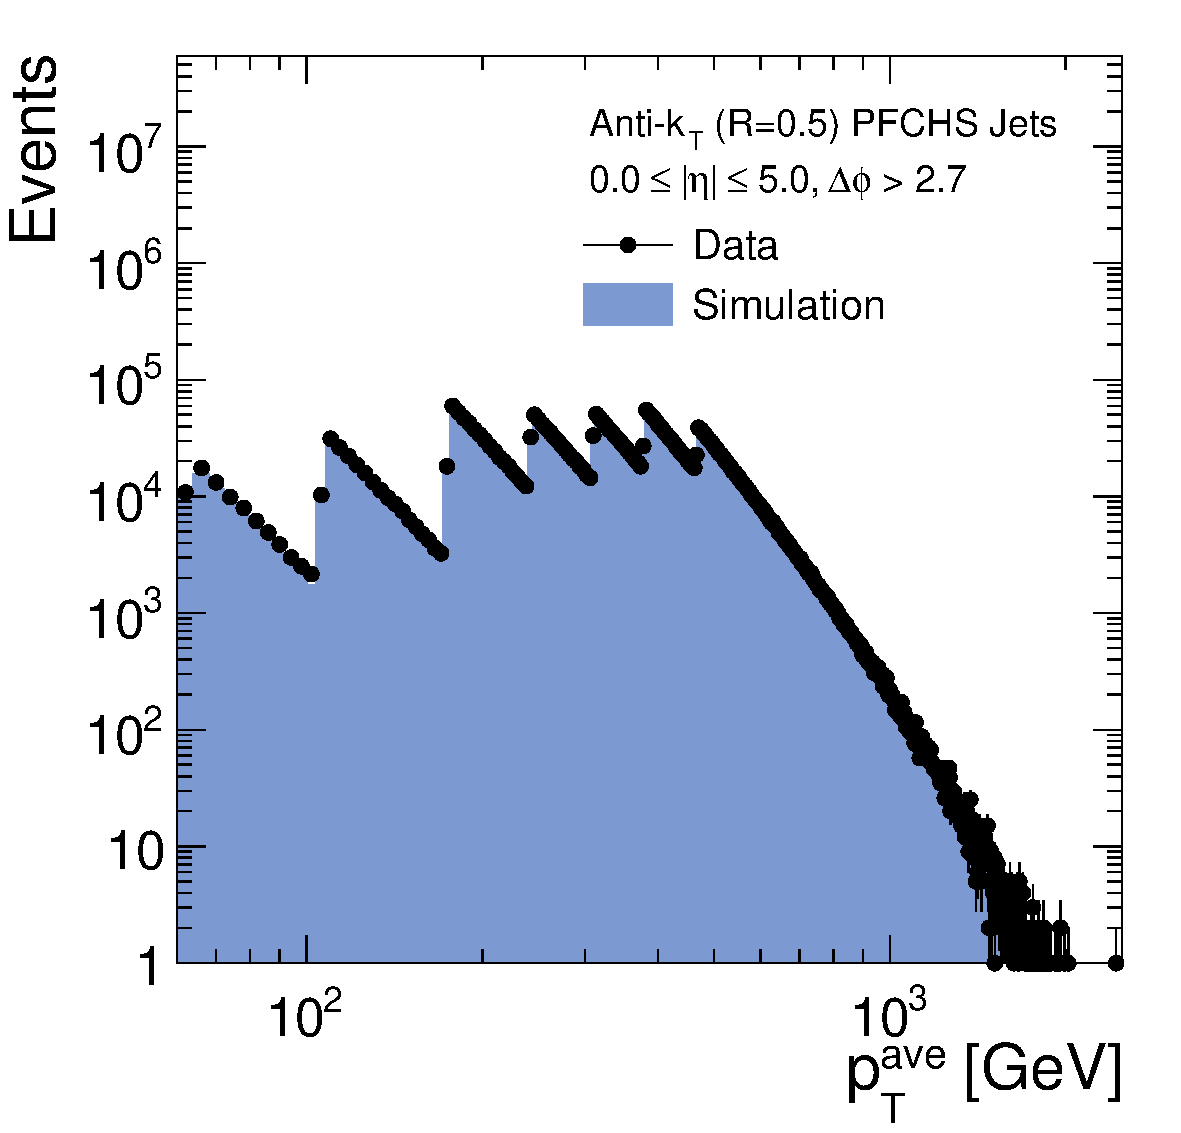
\includegraphics[width=0.49\textwidth]{figures/PtAve__AfterAsymmHistos.pdf} &
                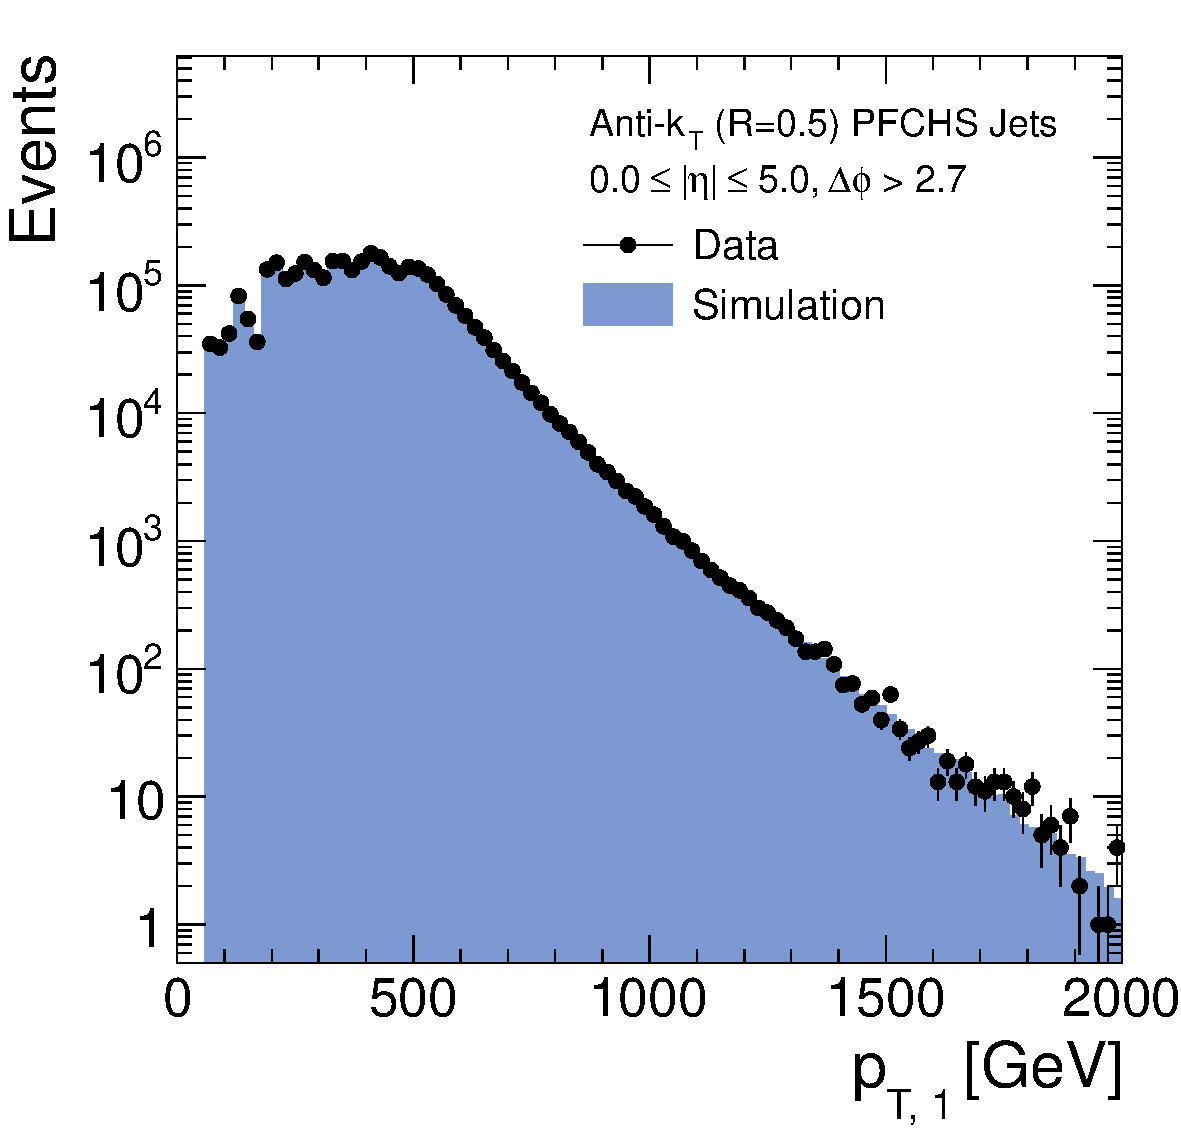
\includegraphics[width=0.49\textwidth]{figures/Jet1Pt__AfterAsymmHistos.pdf} \\
                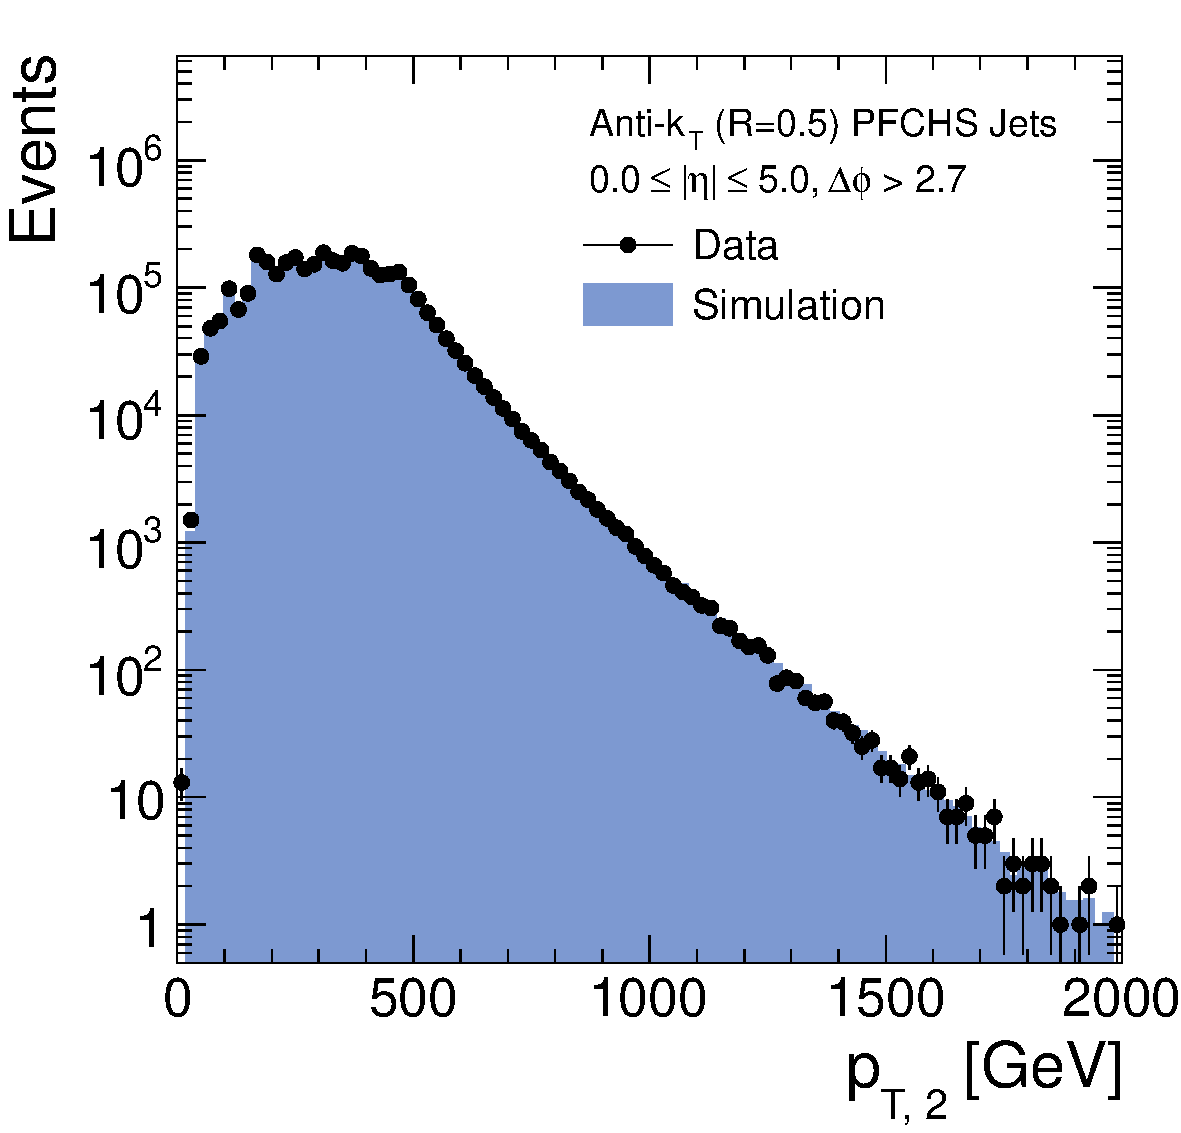
\includegraphics[width=0.49\textwidth]{figures/Jet2Pt__AfterAsymmHistos.pdf} &
                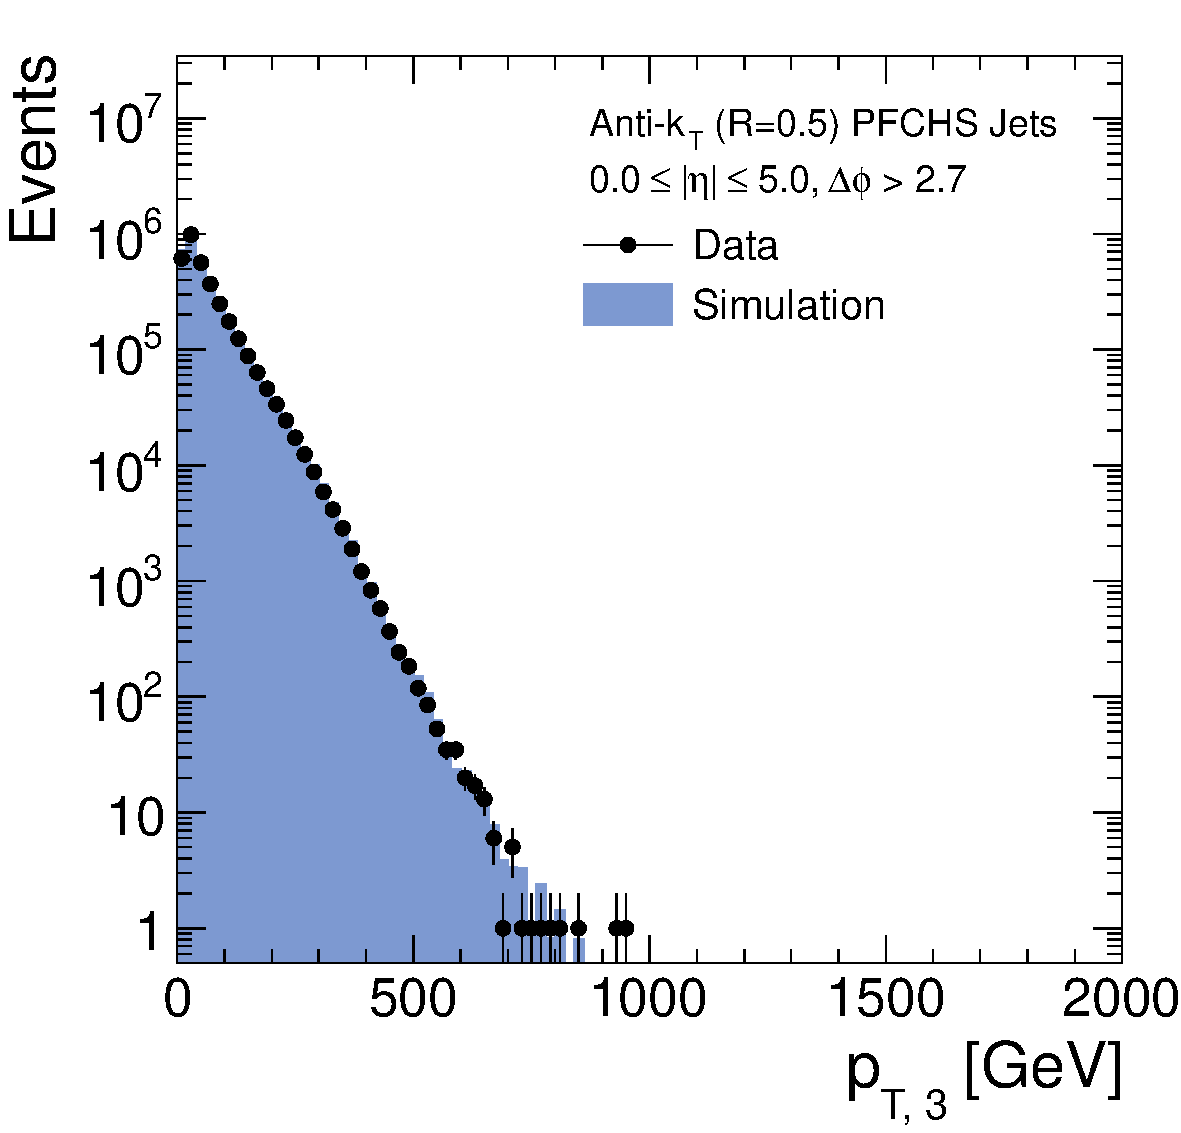
\includegraphics[width=0.49\textwidth]{figures/Jet3Pt__AfterAsymmHistos.pdf}

  \end{tabular}
  \caption{Inclusive $\pt^\mathrm{ave}$ spectrum of events after the total selection in data and in simulation (\textit{top left}), leading jet \pt (\textit{top right}), subleading jet \pt (\textit{bottom left}) and third jet \pt (\textit{bottom right}).}
  \label{fig:ptave_spec}
\end{figure}
\\
Finally, some example asymmetry distributions obtained after the described selection are depicted in Fig.~\ref{fig:asymm_dists} for data and simulated events. They have been obtained using Eq.~\ref{eq:asymmdef}. Instead of randomly assigning the first and second jet, the absolute value of the asymmetry is used. The effect that the asymmetry distribution gets broadened for larger values of $\alpha$ is visible when comparing the distributions in the top and the bottom row. In order to get a robust estimate of the asymmetry width, only asymmetry distributions with at least 100 events in the specified \ptave, $\eta$ and $\alpha$ intervals are considered for the analysis. 
\begin{figure}[!tp]
  \centering
  \begin{tabular}{cc}
                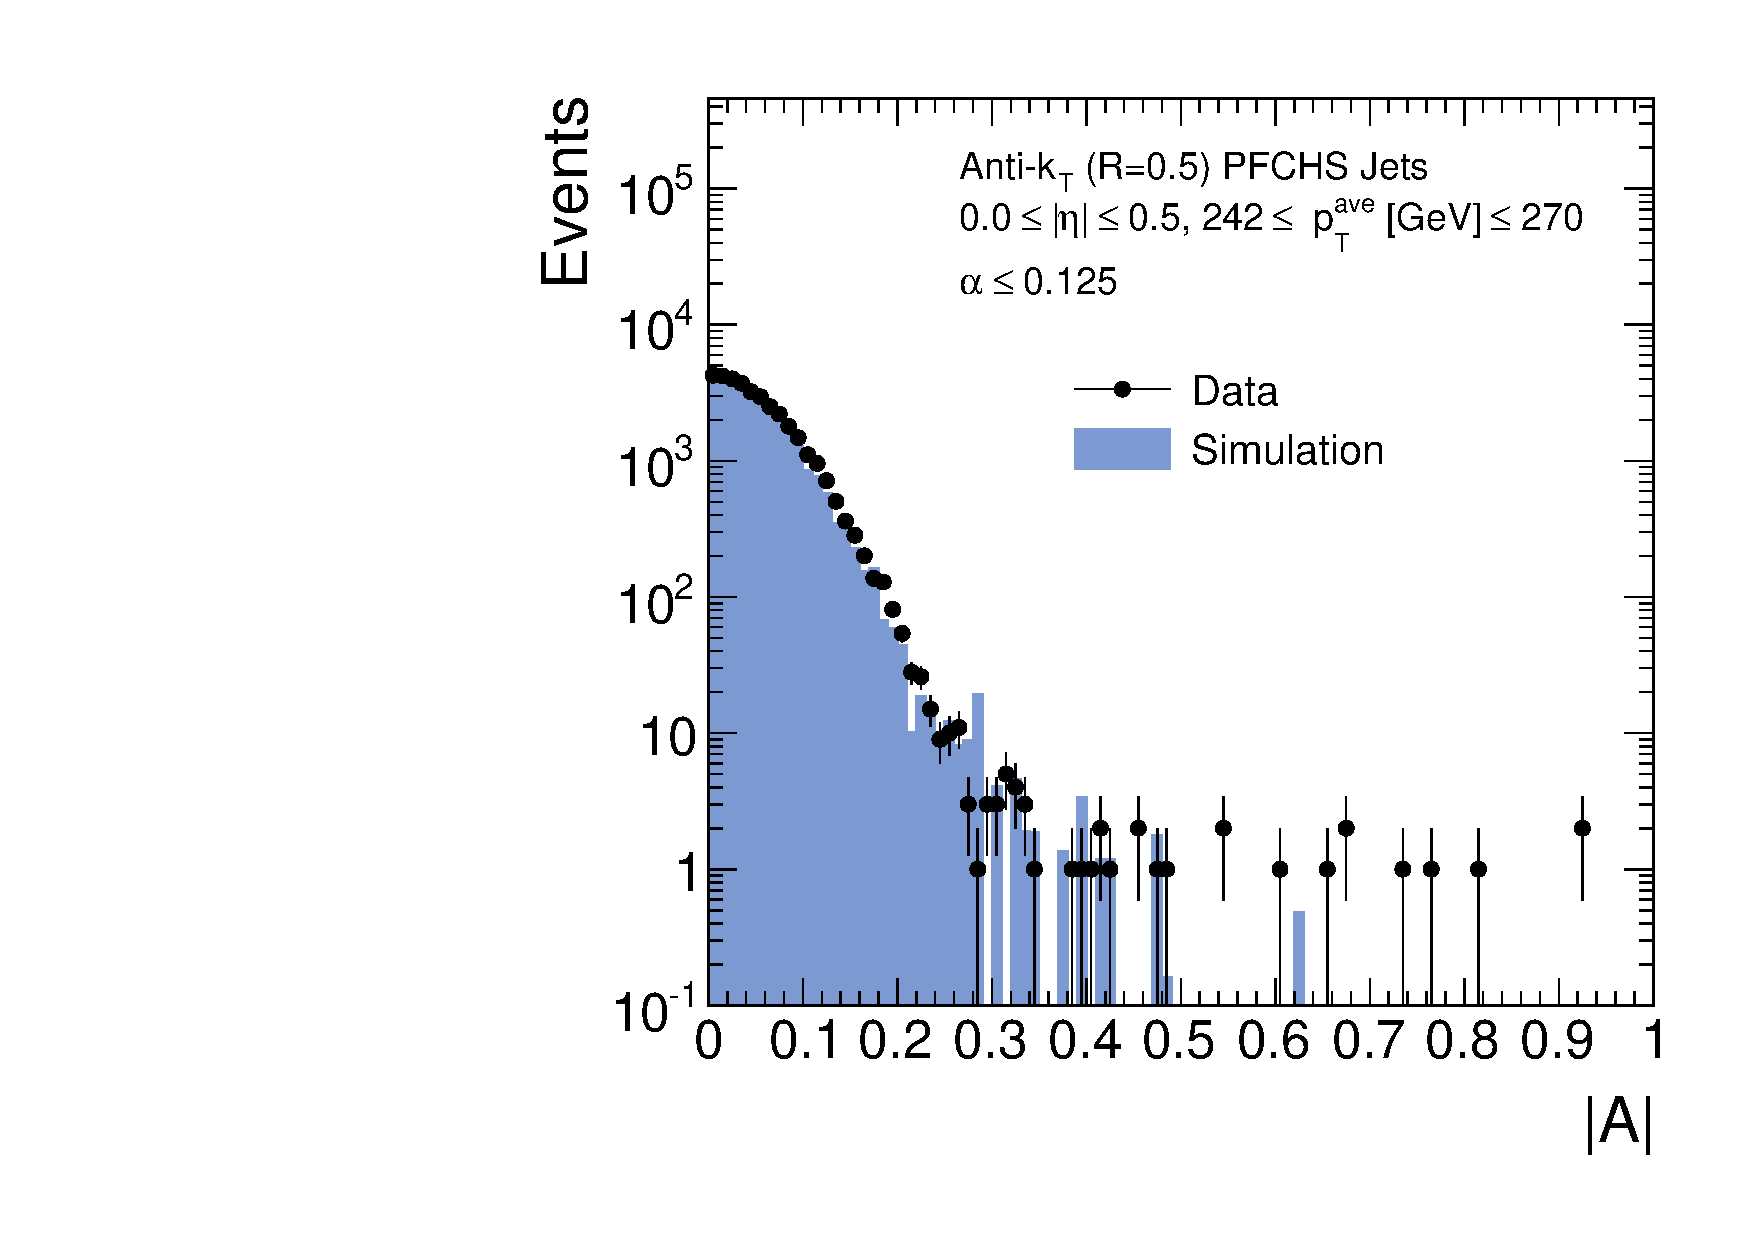
\includegraphics[width=0.49\textwidth]{figures/AsymmHistos_Eta0_pt4_alpha1_final_nominal_v4b.pdf} &
                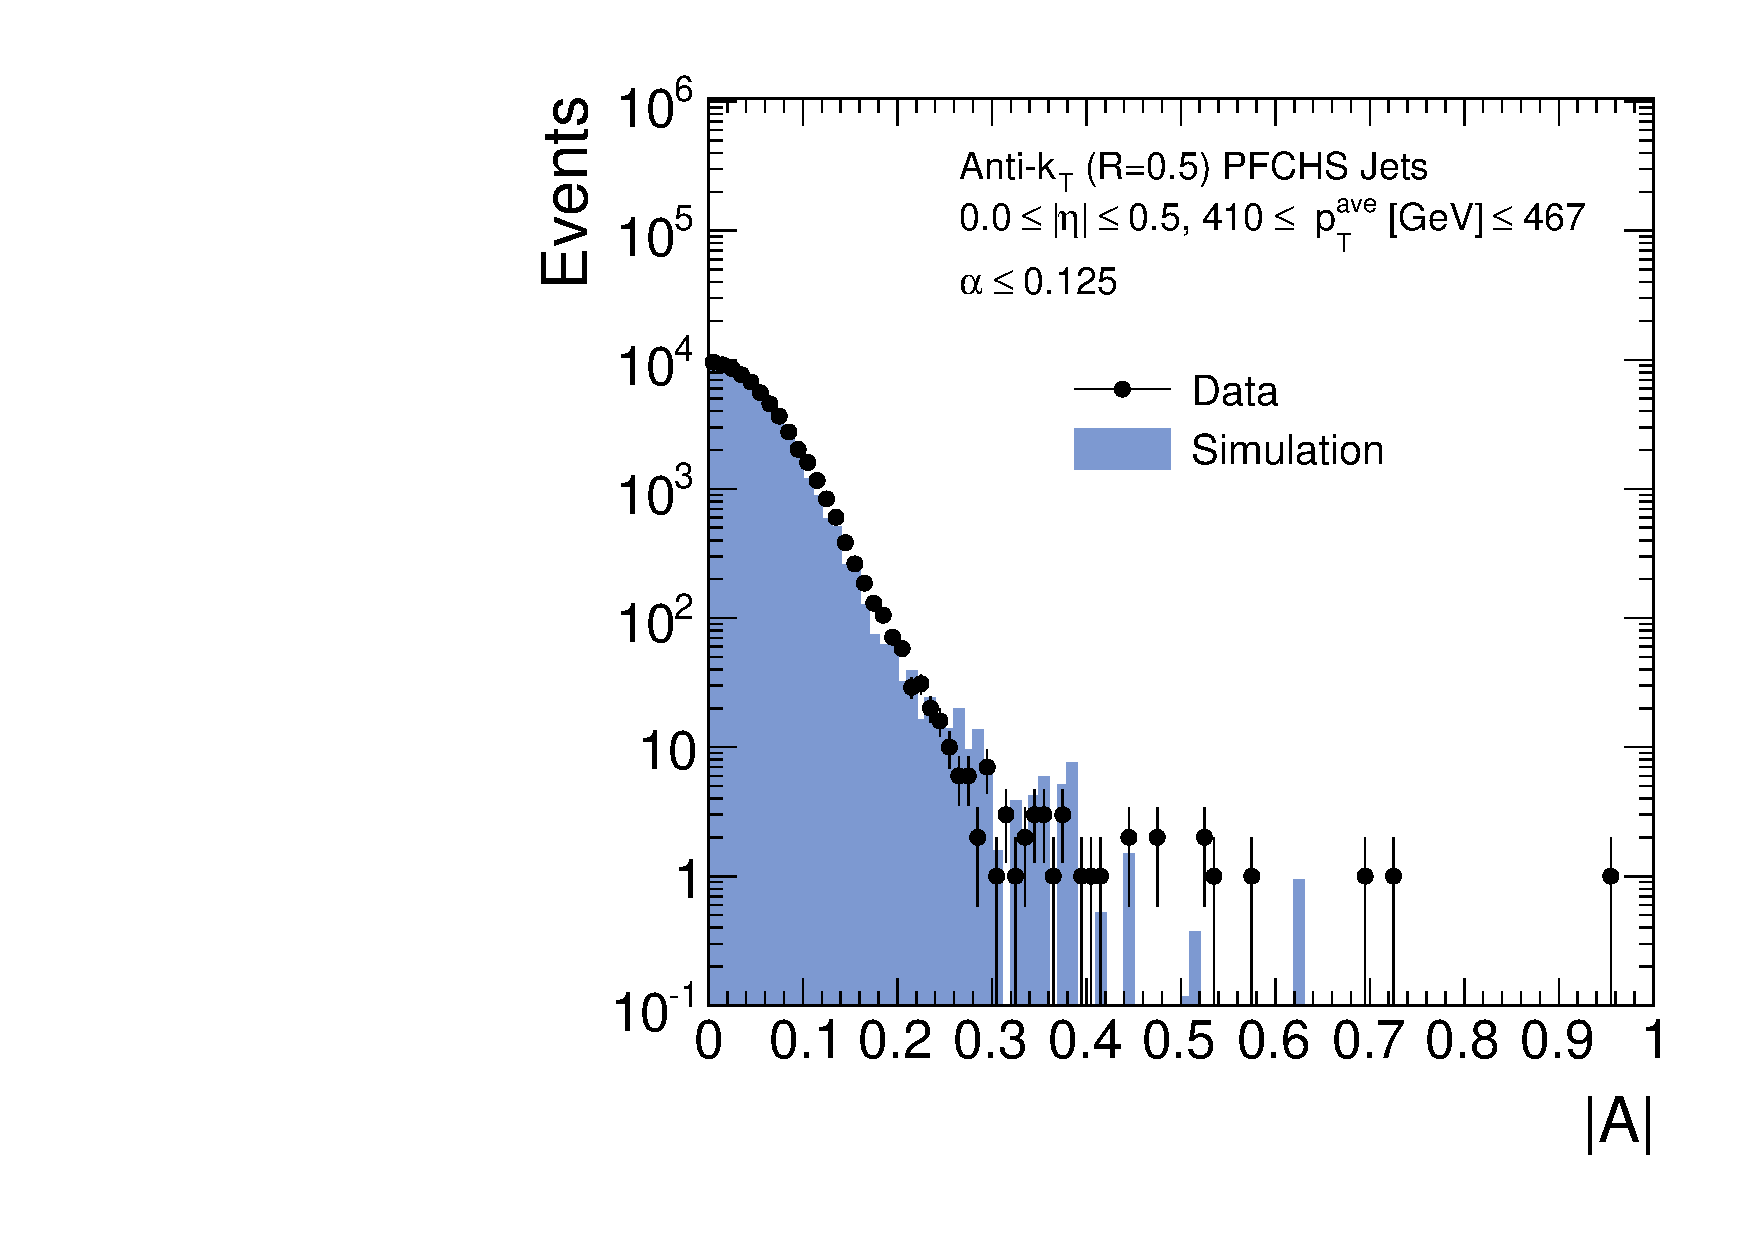
\includegraphics[width=0.49\textwidth]{figures/AsymmHistos_Eta0_pt9_alpha1_final_nominal_v4b.pdf} \\ 
                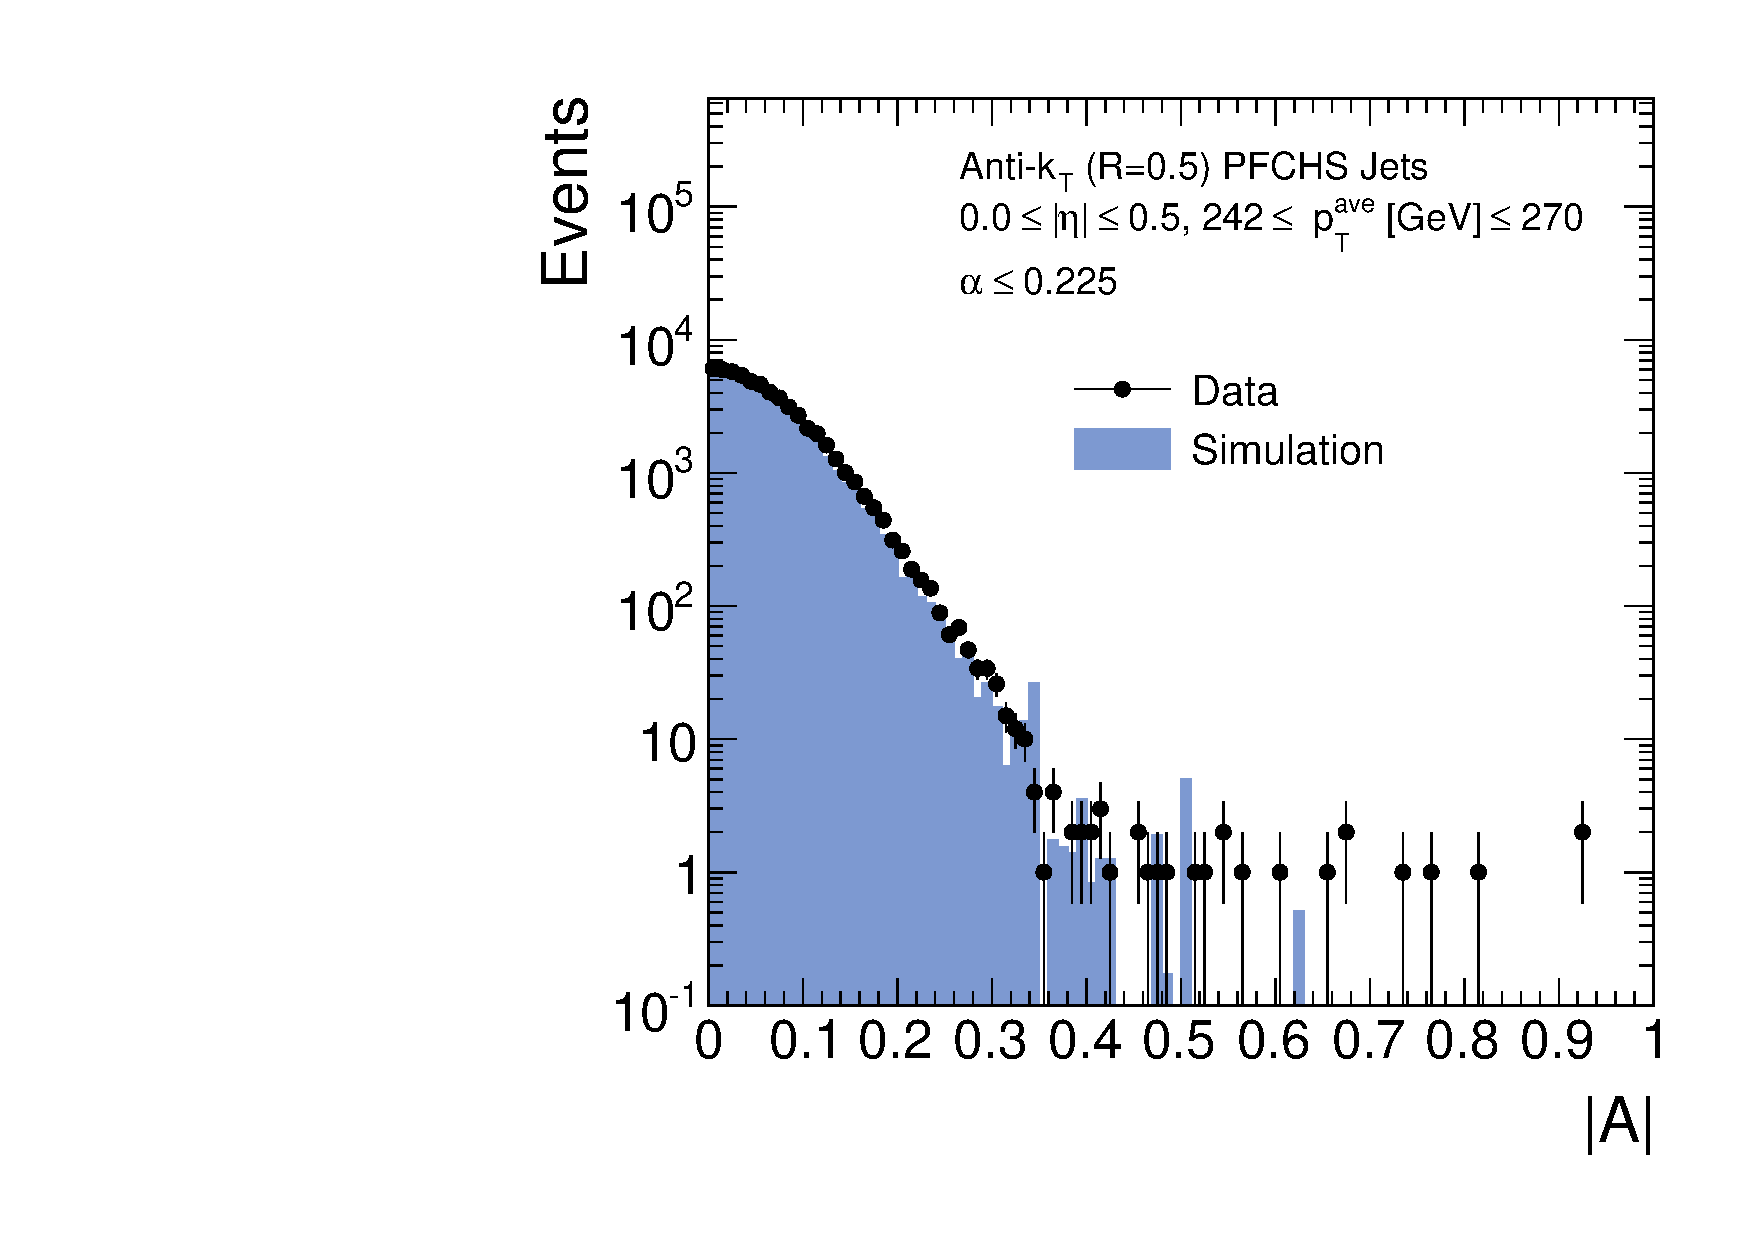
\includegraphics[width=0.49\textwidth]{figures/AsymmHistos_Eta0_pt4_alpha5_final_nominal_v4b.pdf} &
                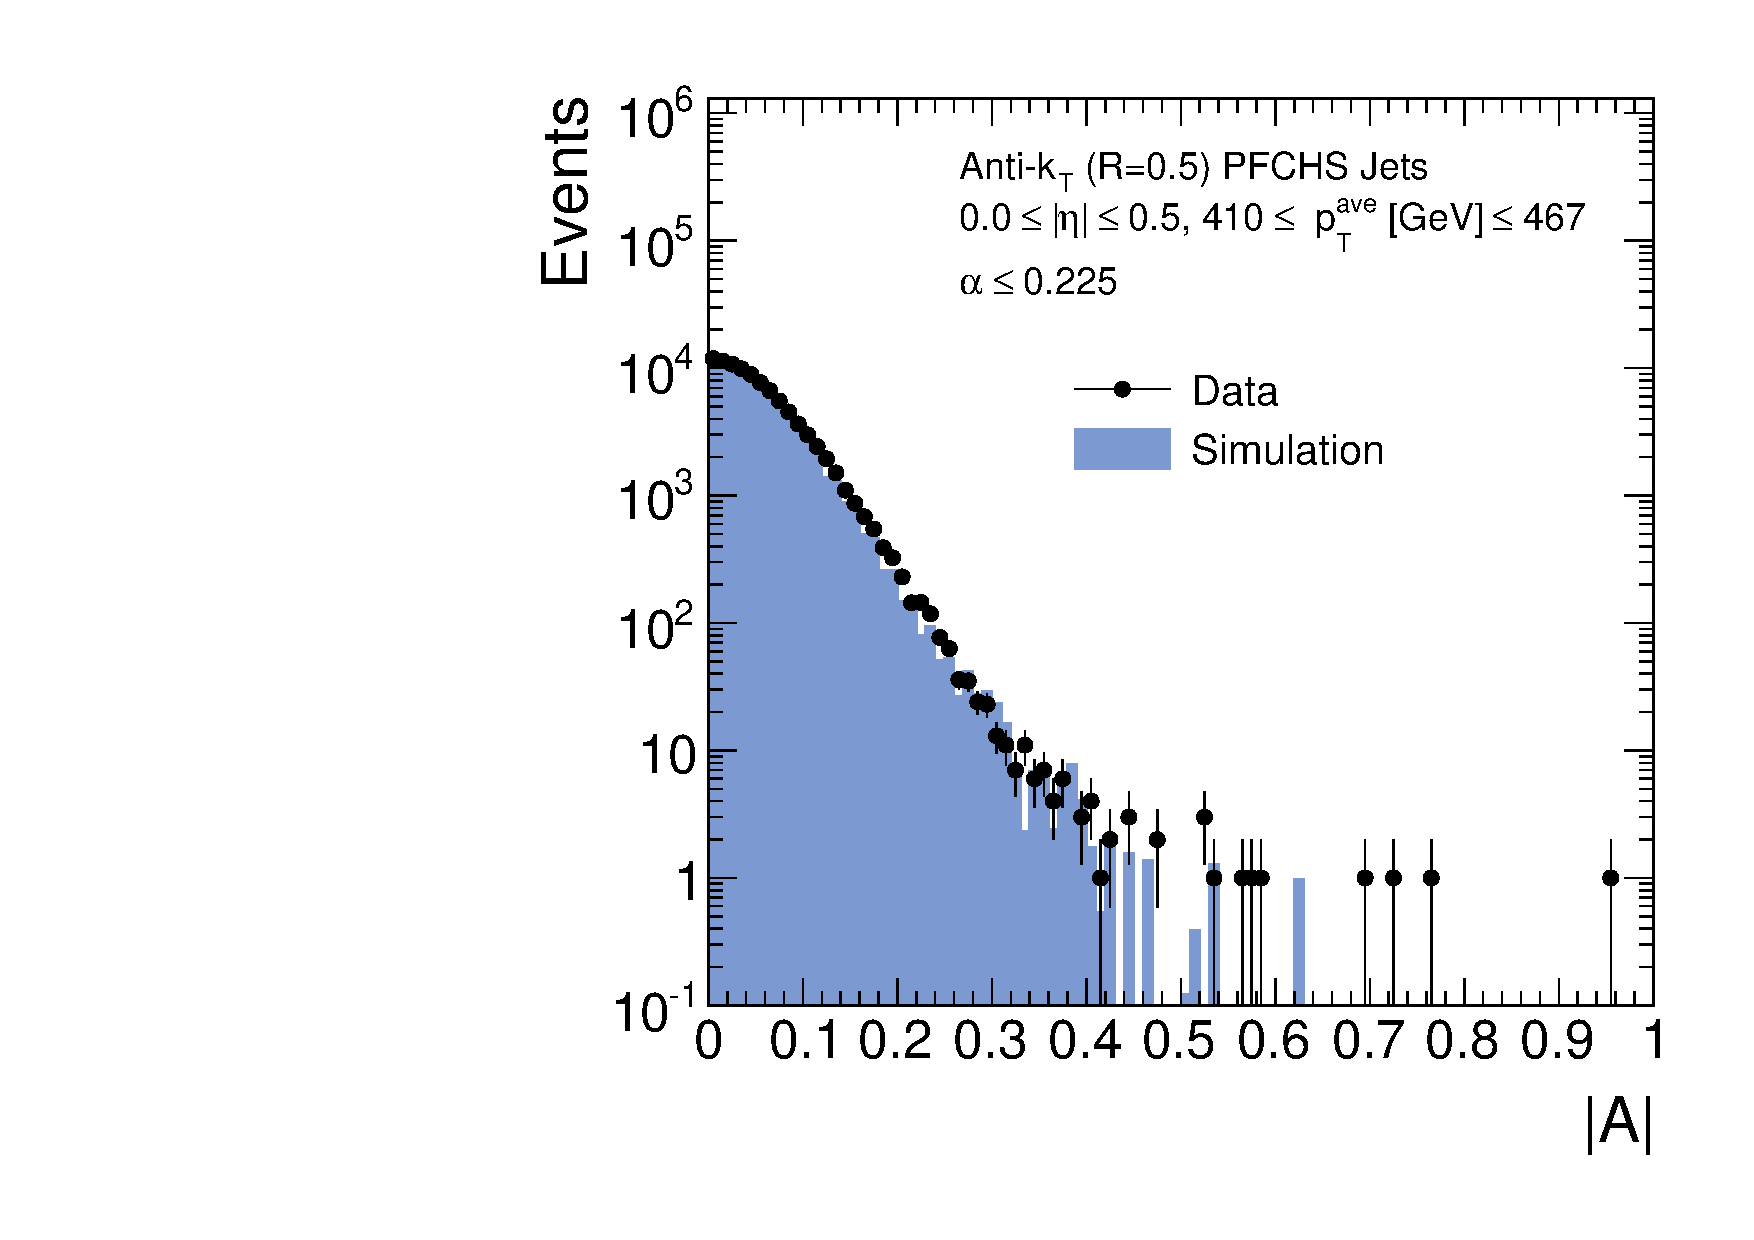
\includegraphics[width=0.49\textwidth]{figures/AsymmHistos_Eta0_pt9_alpha5_final_nominal_v4b.pdf}
  \end{tabular}
  \caption{Some example asymmetry distributions for the lowest $|\eta|$ region, two medium $\pt^\mathrm{ave}$ intervals and for a low (\textit{top}) and a high (\textit{bottom}) $\alpha$ interval.}
  \label{fig:asymm_dists}
\end{figure}

\section{Definition of the Asymmetry Width}
\label{sec:jer_asymm_width_def}
As the measurement of the resolution in collision data is based on the width of the dijet asymmetry distribution, a proper definition of the asymmetry width is needed.\\
From the tails of the jet response, events with large asymmetries can emerge leading to non-Gaussian tails in the asymmetry distributions. These tails have to be rejected in the calculation of the asymmetry width in order to avoid a bias of the measurement. Hence, the asymmetry width has to be defined such that the core part of the distribution is described. Since the core of the asymmetry distribution is expected to be Gaussian-shaped, a proper description of the asymmetry core can be tested by comparing the actual asymmetry histogram to a Gaussian function. The standard deviation of the Gaussian function can be chosen according to different definitions of the width of the asymmetry distribution and so the definition of the asymmetry width can be identified which features a good description of the asymmetry distribution by a corresponding Gaussian function. \\
\begin{figure}[!htp]   
  \centering
  \begin{tabular}{cc}
                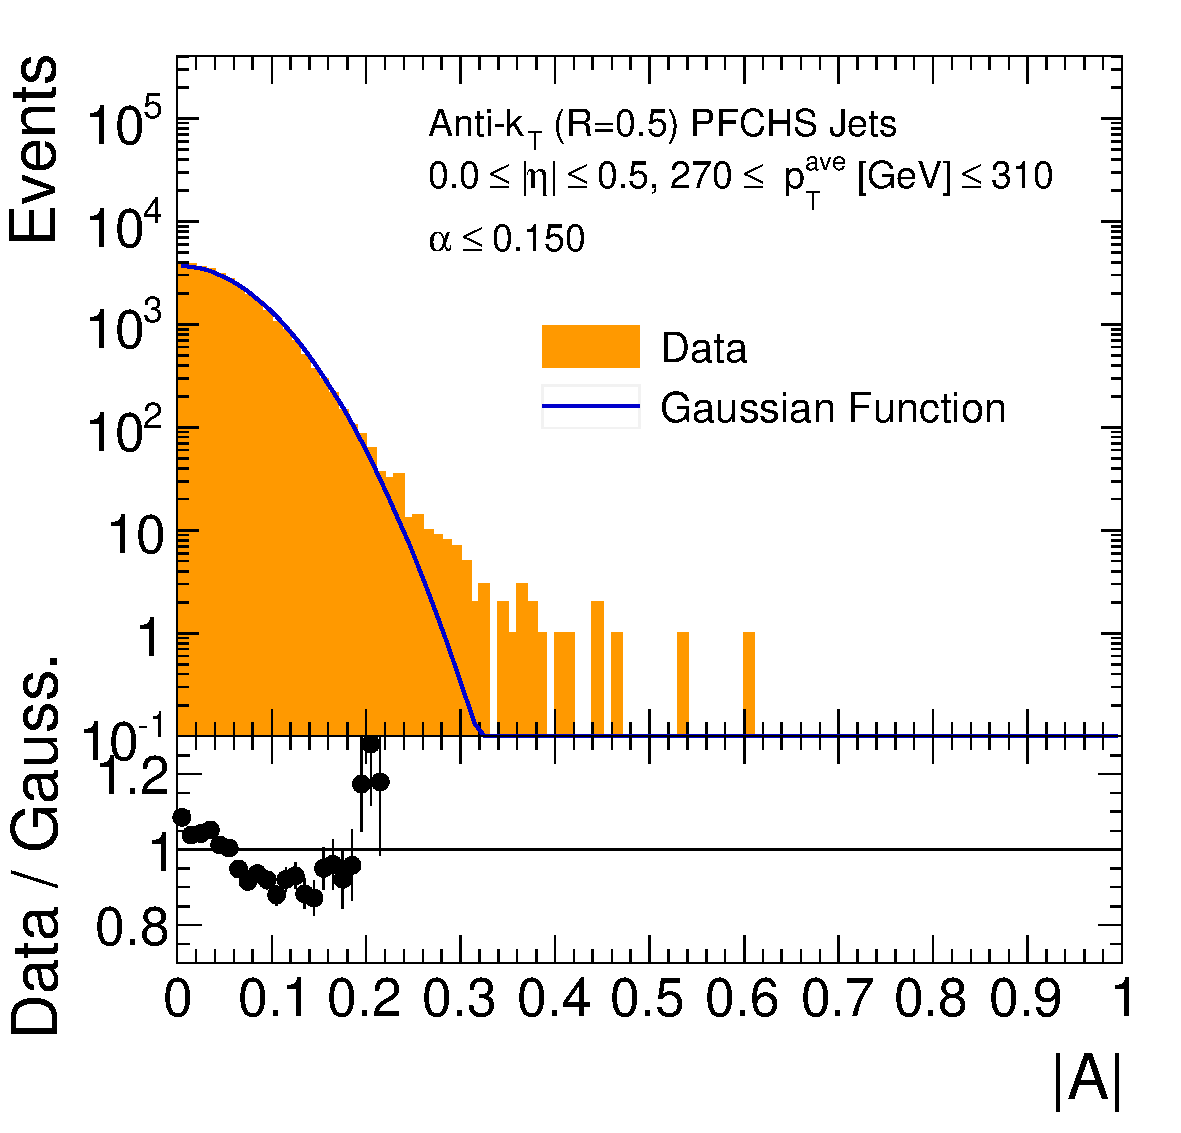
\includegraphics[width=0.49\textwidth]{figures/AsymmHistosDataWithRatio_Eta0_pt5_alpha2_final_nominal_NoTruncation_v4.pdf} &
                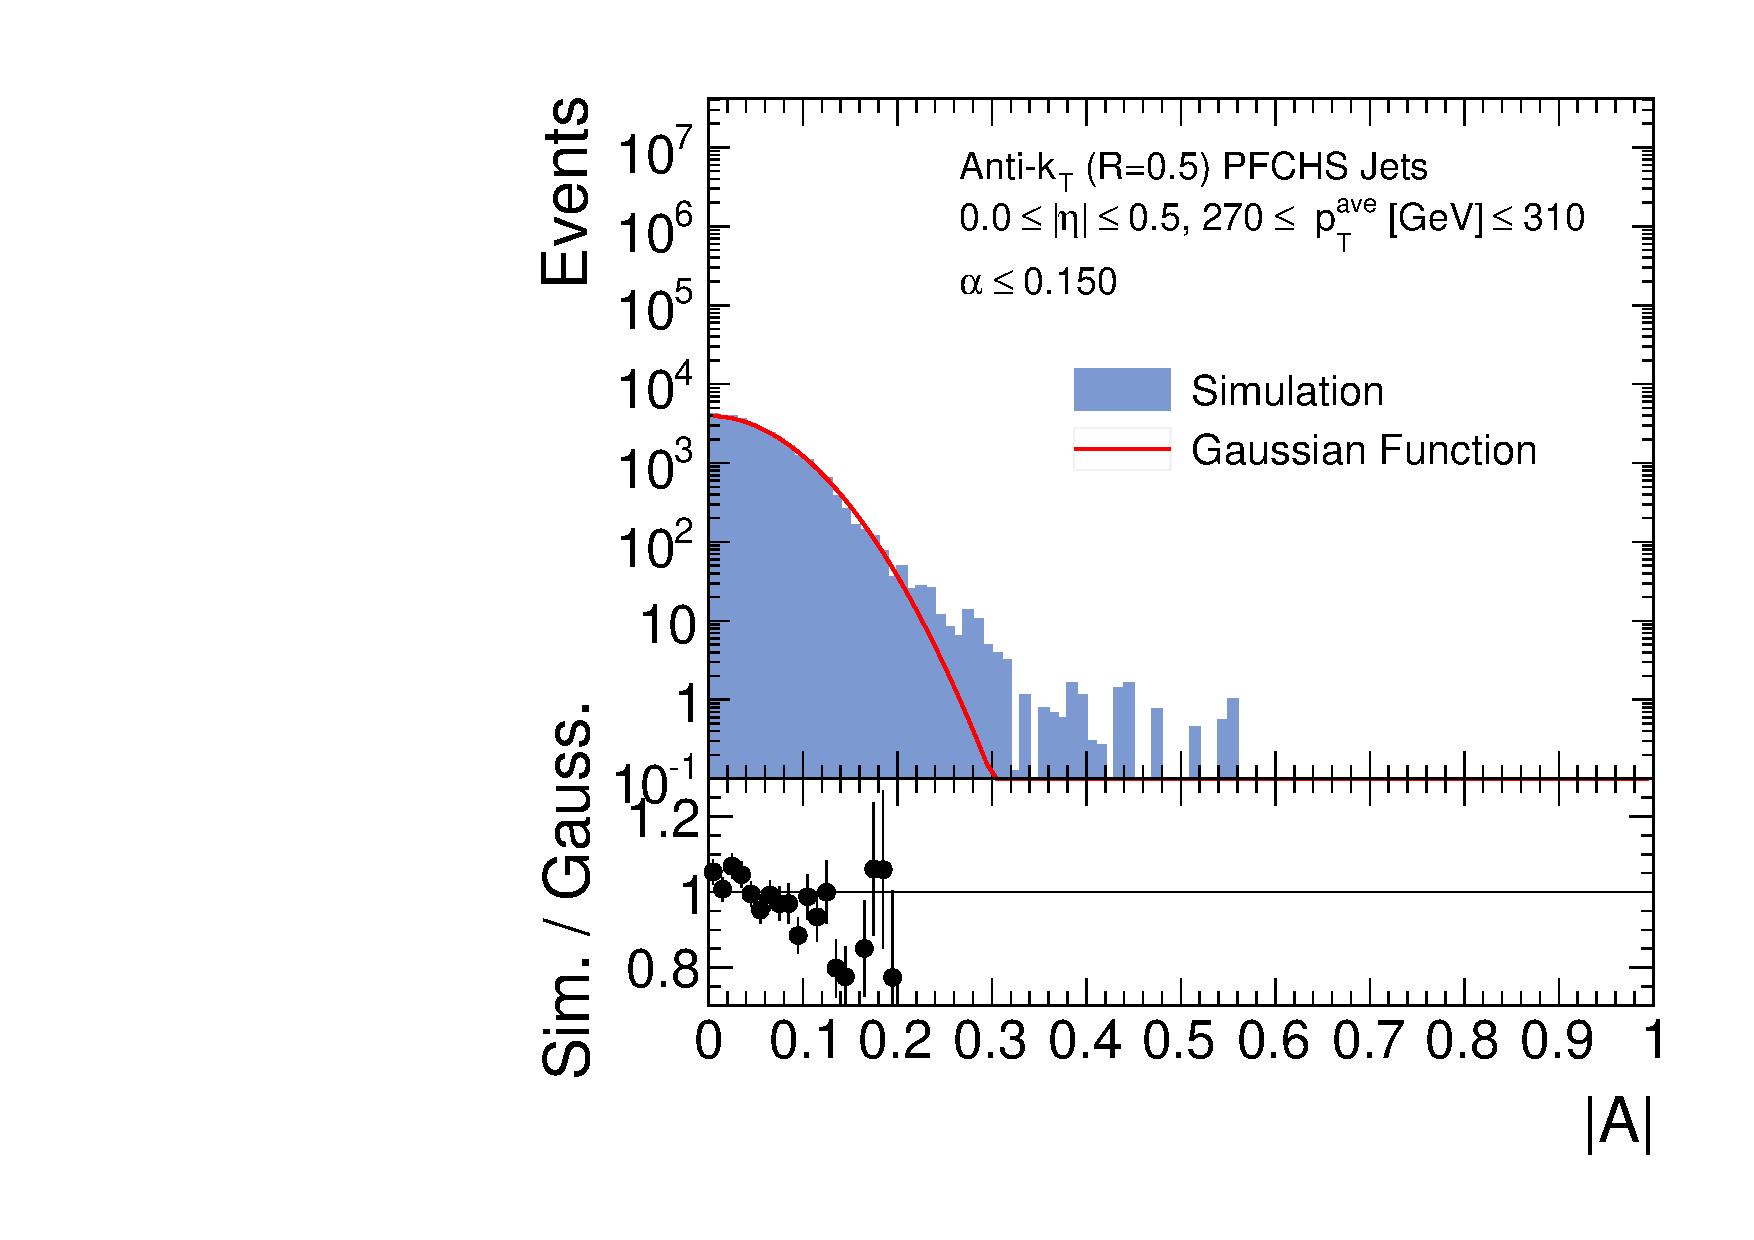
\includegraphics[width=0.49\textwidth]{figures/AsymmHistosSimWithRatio_Eta0_pt5_alpha2_final_nominal_NoTruncation_v4b.pdf} \\ 
                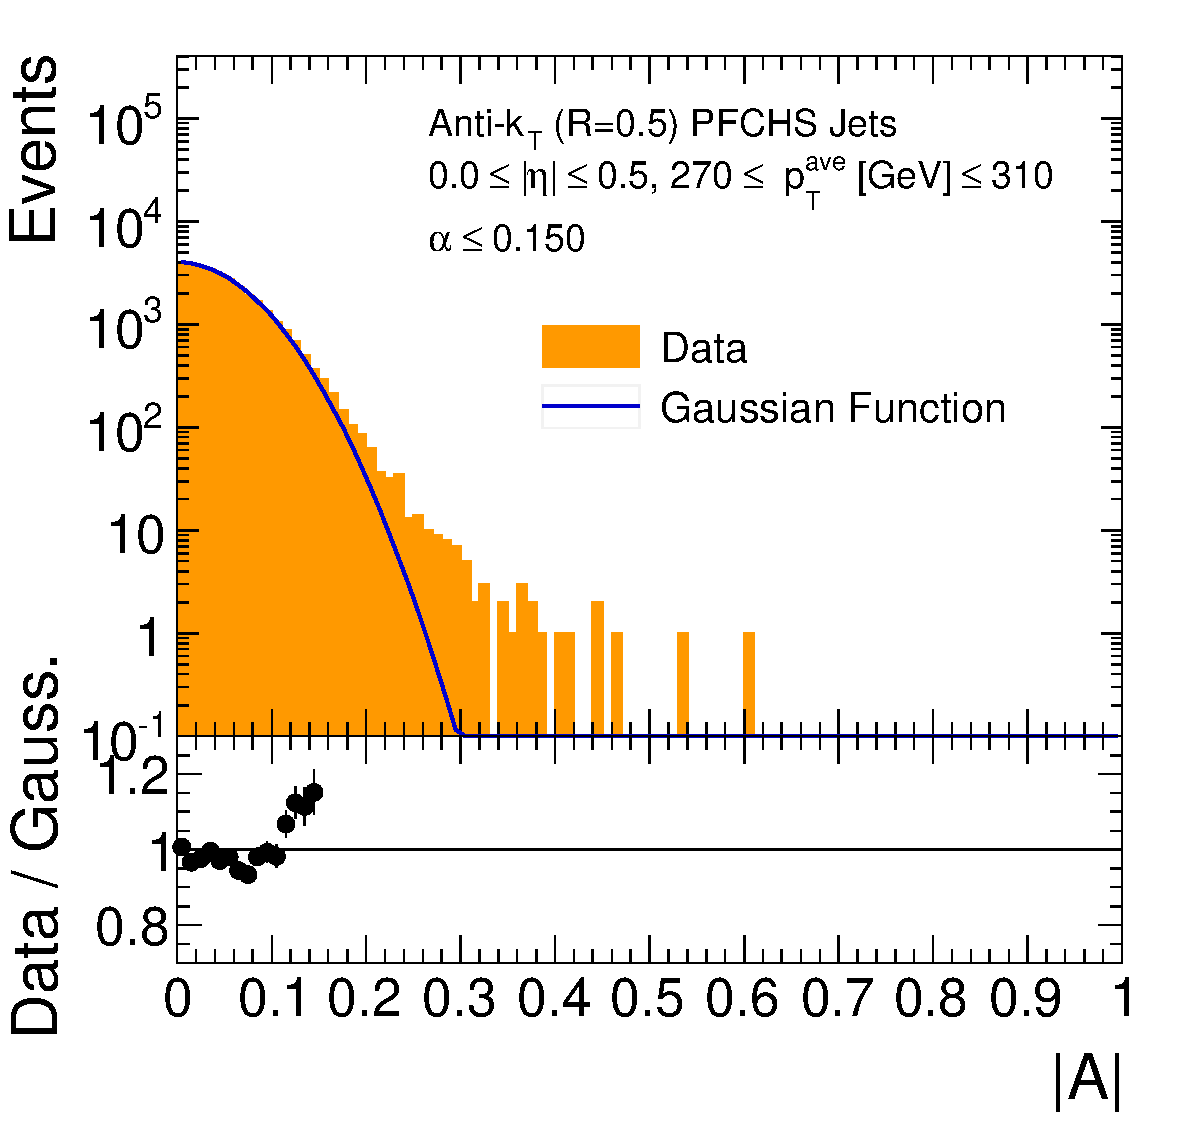
\includegraphics[width=0.49\textwidth]{figures/AsymmHistosDataWithRatio_Eta0_pt5_alpha2_final_nominal_v4.pdf} &
                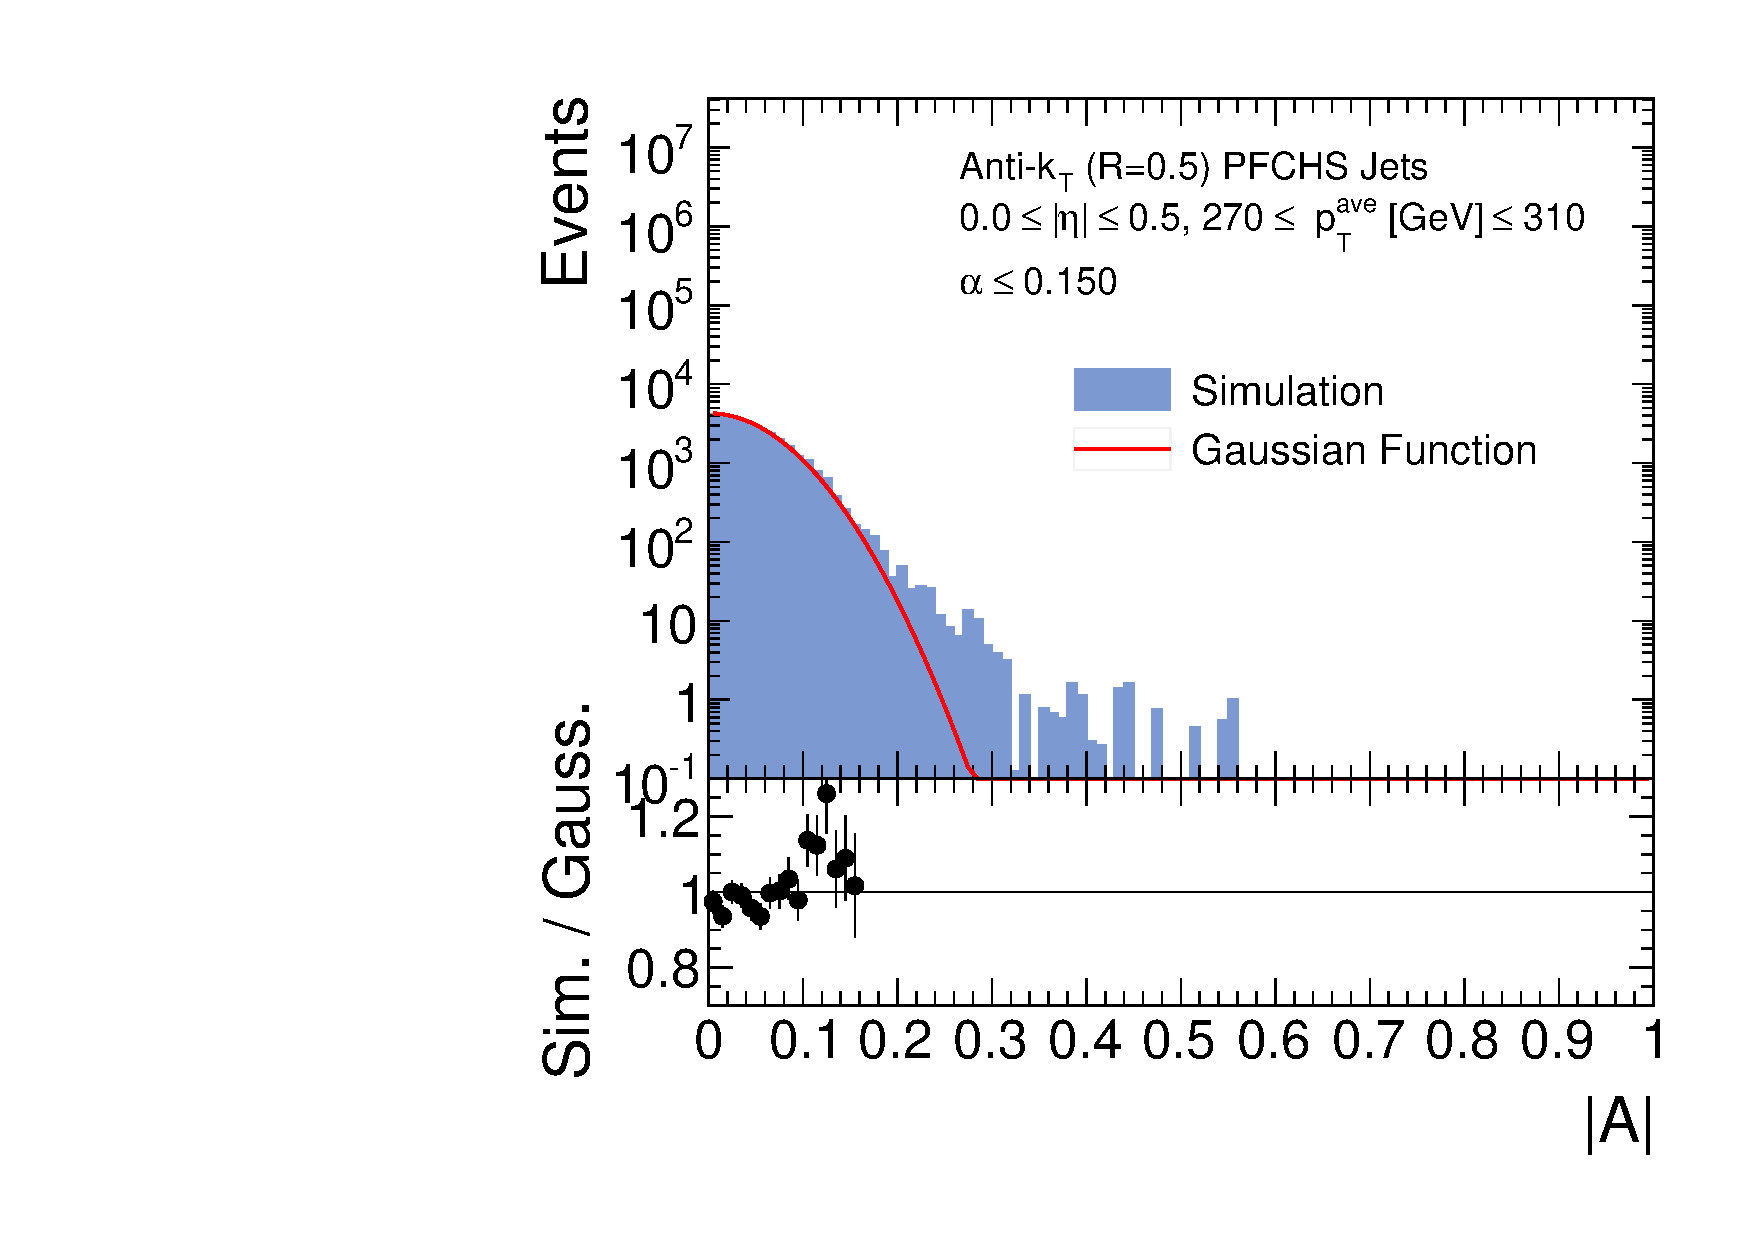
\includegraphics[width=0.49\textwidth]{figures/AsymmHistosSimWithRatio_Eta0_pt5_alpha2_final_nominal_v4b.pdf} \\
                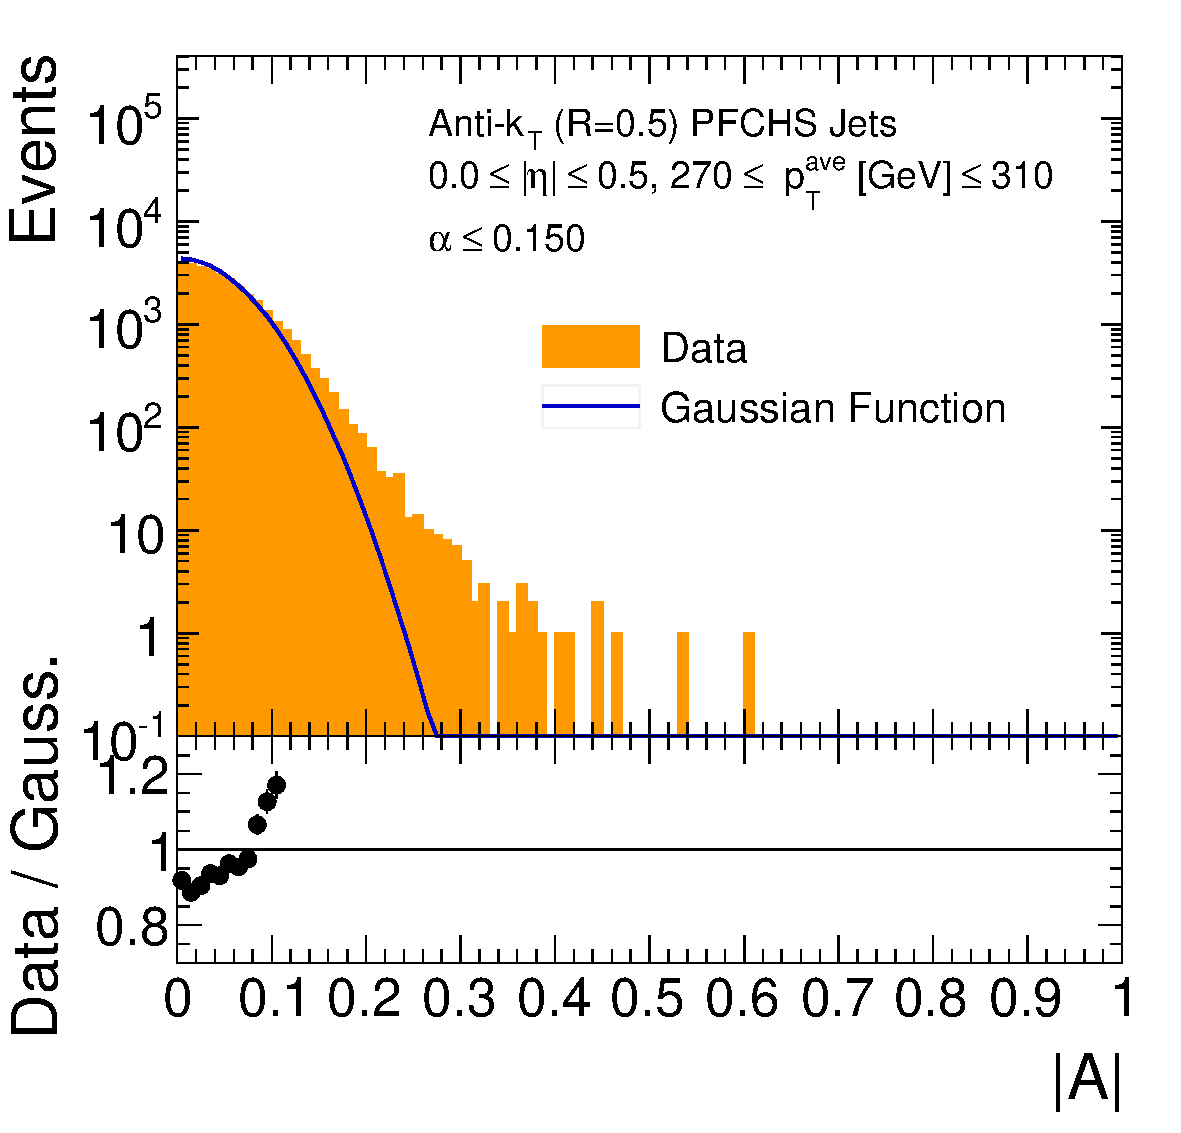
\includegraphics[width=0.49\textwidth]{figures/AsymmHistosDataWithRatio_Eta0_pt5_alpha2_final_nominal_95Truncation_v4.pdf} &
                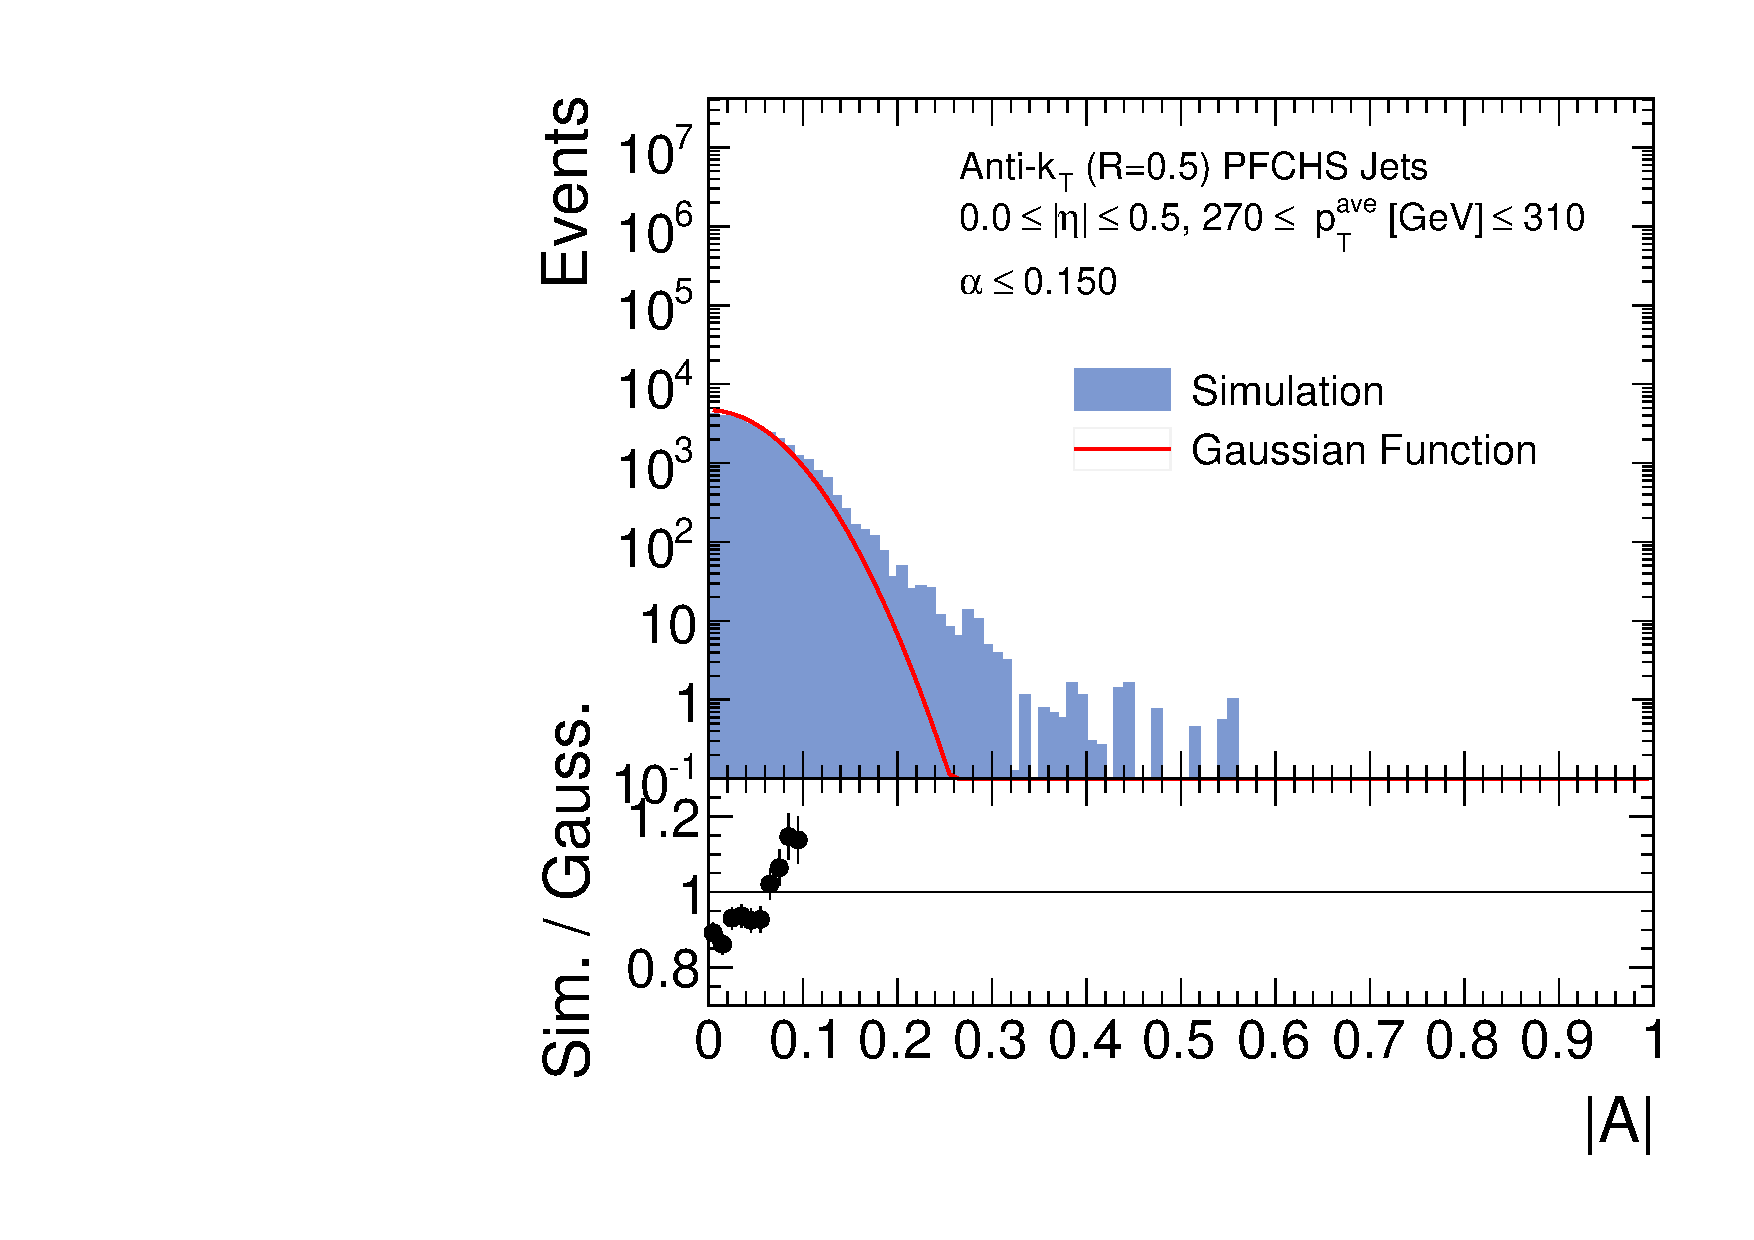
\includegraphics[width=0.49\textwidth]{figures/AsymmHistosSimWithRatio_Eta0_pt5_alpha2_final_nominal_95Truncation_v4b.pdf} \\
  \end{tabular}
  \caption{Asymmetry distributions for data (\textit{left}) and simulation (\textit{right}) compared to Gaussian distributions obtained with standard deviations corresponding to 0\% truncation (\textit{top}), 1.5\% truncation (\textit{middle}) and 5\% truncation (\textit{bottom}) of the respective upper tail.}
  \label{fig:asymm_width}
\end{figure}
The width of the asymmetry is determined by taking the whole distribution into account or by truncating a certain percentage of the tail regions. Thus, the asymmetry width is calculated as truncated root-mean-square
\begin{equation}
 \sigma_\mathrm{A} = \mathrm{RMS}_{t\%} = \sqrt{\frac{1}{\sum_{i} y_i} \sum_{i} y_i \cdot A_i^2}  
 \label{eq:truncated_rms}
\end{equation} 
where $y_i$ denotes the frequency of the asymmetry value $A_i$ and the sum over $i$ includes all values such that the total asymmetry distribution is covered from zero up to a percentage $t$. Assuming a normal distribution, the statistical uncertainty is given by
\begin{equation}
\Delta \sigma_\mathrm{A} = \Delta \mathrm{RMS}_{t\%} = \frac{\mathrm{RMS}_{t\%}}{\sqrt{\, 2 \cdot n_\mathrm{eff}}} \,
\end{equation} 
with the number of effective entries $n_\mathrm{eff}$\footnote{In case of an unweighted histogram, $n_\mathrm{eff}$ is equivalent to the number of histogram entries. However, for a weighted histogram, as \eg in simulation, $n_\mathrm{eff}$ corresponds to the hypothetical number of unweighted entries a histogram would need, in order to have the same statistical power as the weighted histogram.} in the specified (\ptave, $|\eta|$, $\alpha$)-interval. The truncation is chosen such that the whole distribution, $98.5\%$ or only $95\%$ are considered. A comparison of the asymmetry distributions and Gaussian functions where the standard deviation has been set to the value of the determined asymmetry width is illustrated in Fig.~\ref{fig:asymm_width} for a certain $|\eta|$, $\pt^\mathrm{ave}$ and $\alpha$ interval. It is visible that the core part of the asymmetry distribution can in good approximation be described by a Gaussian function when choosing $\mathrm{RMS}_{98.5\%}$ as the asymmetry width (\cf middle row in Fig.~\ref{fig:asymm_width}). Hence, this is the default definition of the asymmetry width used for this measurement. It is chosen to be the same for data events as well as for simulated events.  

\section{Corrections to the Dijet Asymmetry}
\label{sec:jer_corrections}
The fundamental relation between the width of the asymmetry distribution and the jet energy resolution as expressed in Eq.~\ref{eq:asymm} holds in this form only for the case of an ideal dijet topology. In real collision events, various effects occur that disturb the exact balance of the two jets as discussed in Section~\ref{sec:jer_application}. Such effects can be soft radiation or additional jets originating from the hard scattering. They lead to momentum imbalance in the event and hence broaden the measured asymmetry distribution which consequently also results in an increased measured jet resolution. In order to determine the intrinsic resolution, the measured asymmetry width has to be corrected for such effects. These corrections are explained in the following Sections~\ref{subsec:jer_corrections_alpha} and~\ref{subsec:jer_corrections_pli}.

\subsection{Correction for Additional Jet Activity}
\label{subsec:jer_corrections_alpha}
%In addition to the two jets originating from the hard interaction, further jets can occur in an event from the emission of additional partons. The additional jet activity in the event is quantified by $\alpha$ introduced in Eq.~\ref{eq:alpha} which is the fractional \pt of the third jet. The impact from jets beyond the third one is neglected since there impact is expected to be small due to the strongly decreasing jet-production cross-section. \\
The imbalance contribution arising from additional jet activity is taken care of by an extrapolation procedure. As described in Section~\ref{subsec:jer_sel_cuts}, the asymmetry distribution is calculated for several intervals in $|\eta|$ and $\pt^\mathrm{ave}$ with different selections on the maximum value of $\alpha$ ($=\alpha_{max}$). For each of these individual selections, the width of the asymmetry is determined as stated in Section~\ref{sec:jer_asymm_width_def}. The measured values of $\sigma_{A}(\alpha_{max})$ are extrapolated to $\alpha_{max} \rightarrow 0$ assuming a linear behaviour. Thus, the measured asymmetry widths in one particular ($\pt^\mathrm{ave}$, $|\eta|$, $\alpha$)-interval are fitted with a linear function. The $y$-intercept of the fitted linear function represents the resolution without further jet activity in the event. The statistical uncertainty is given by the respective fit uncertainty for the intercept. \\
The extrapolation procedure for two exemplative $|\eta|$ and $\pt^\mathrm{ave}$ intervals is illustrated in Fig.~\ref{fig:extrapol}. The performed extrapolation fits for all other non-empty intervals are shown in App.~\ref{app:extrapolations}. 
\begin{figure}[!tp]
  \centering
  \begin{tabular}{cc}
                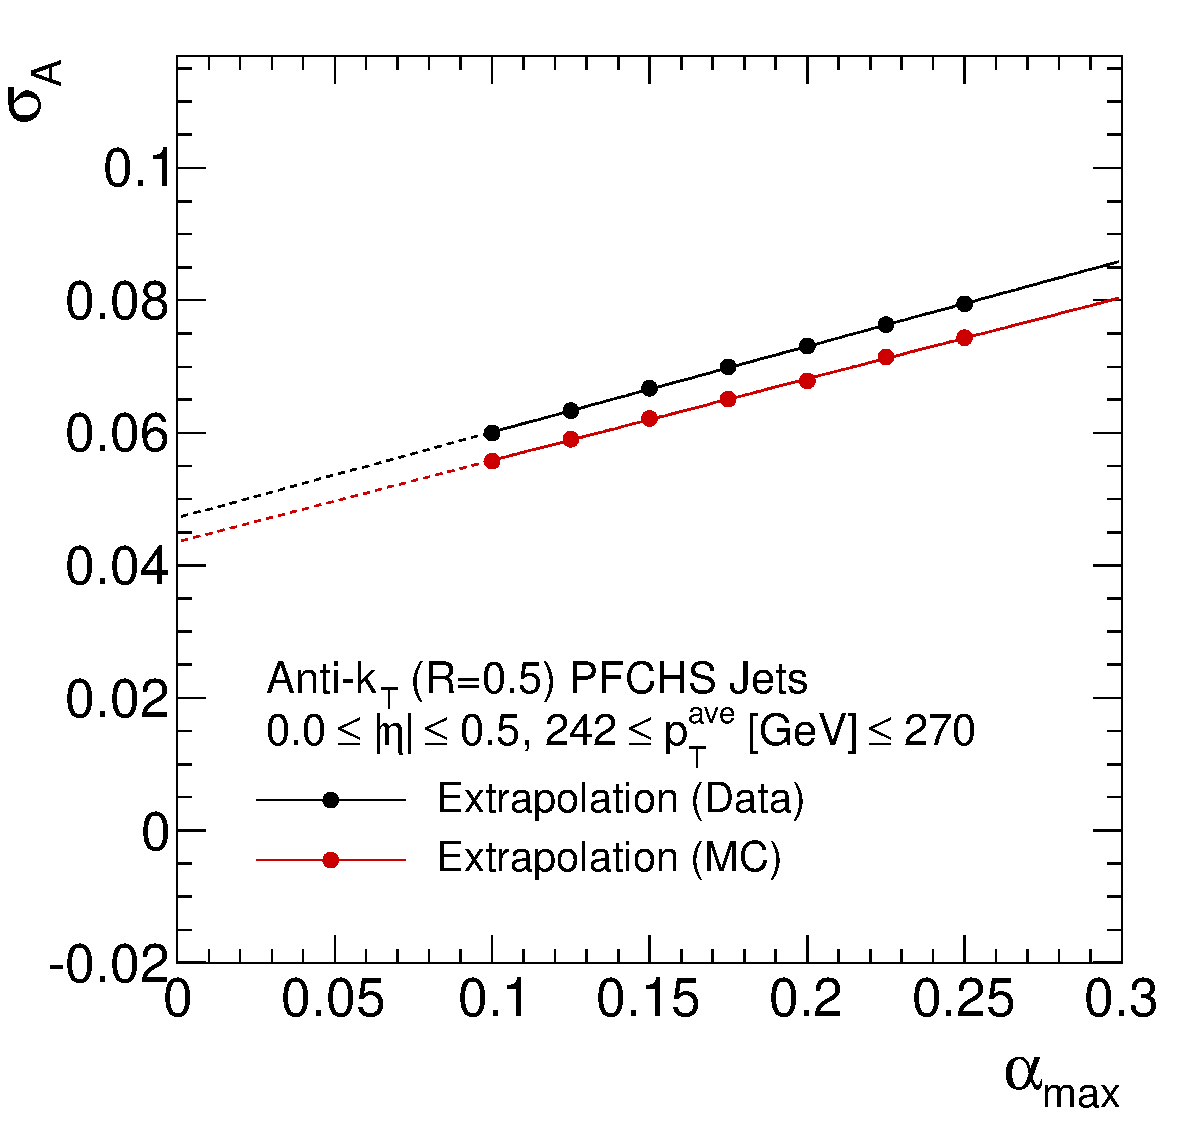
\includegraphics[width=0.49\textwidth]{figures/Extrapol_Eta0_pt4_final_nominal_v4.pdf} &
                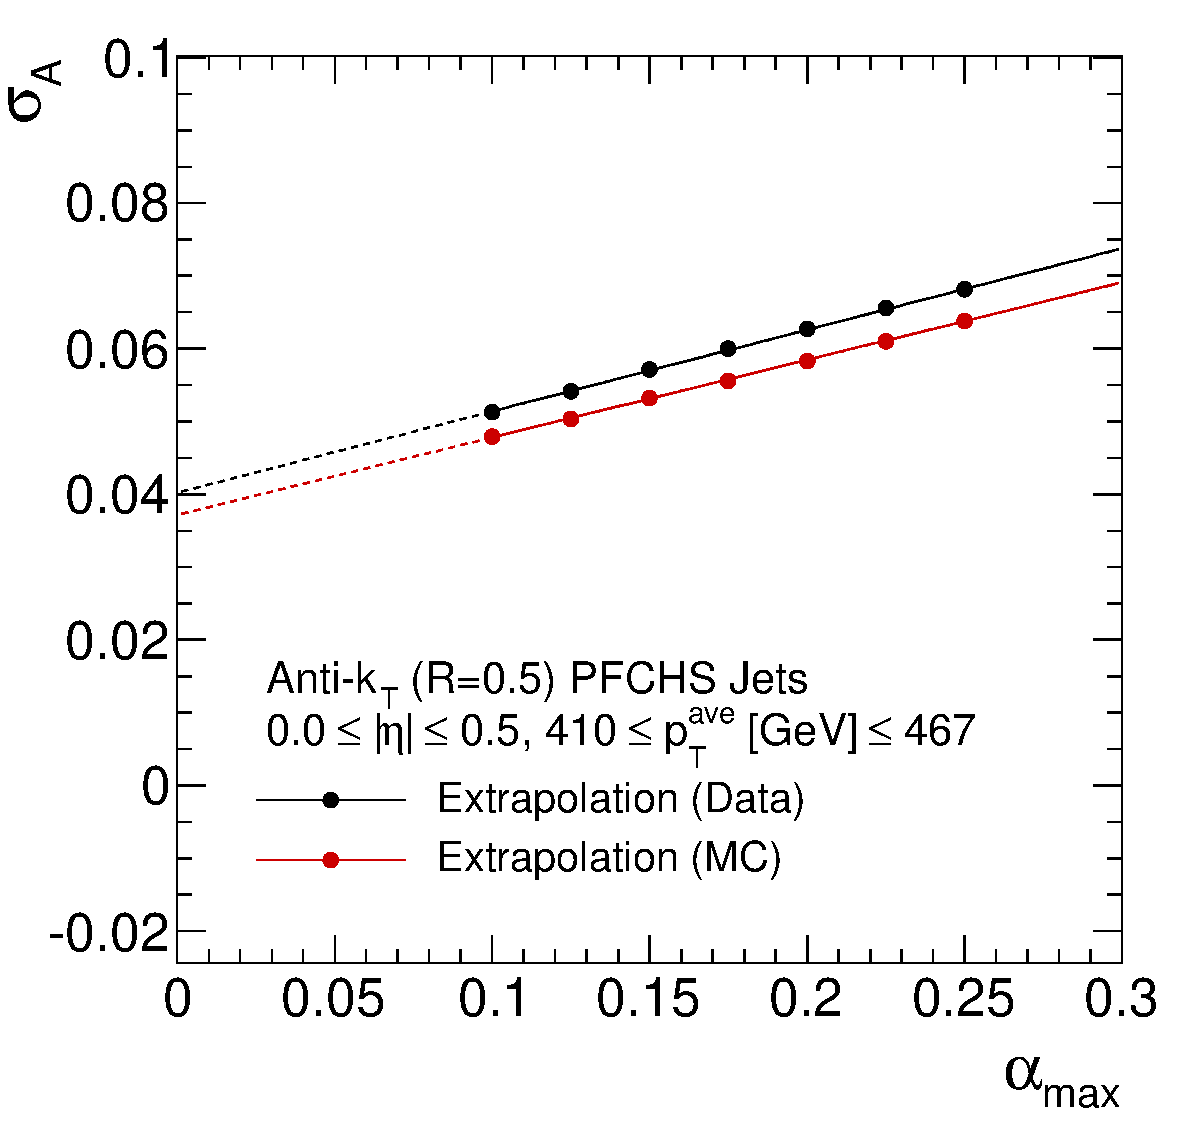
\includegraphics[width=0.49\textwidth]{figures/Extrapol_Eta0_pt9_final_nominal_v4.pdf}
  \end{tabular}
  \caption{Two example extrapolations of measured values for $\sigma_\mathrm{A}$ in data (black) and simulation (red) to obtain the asymmetry width for zero additional jet activity.}
  \label{fig:extrapol}
\end{figure}
\\
As stated in Section~\ref{subsec:jer_sel_cuts}, the selection is performed in inclusive intervals of $\alpha < \alpha_\mathrm{max}$. This results in a correlation of the measured values of $\sigma_\mathrm{A}$ for a particular ($\pt^\mathrm{ave}$, $|\eta|$)-interval. In order to obtain a proper estimate of the statistical uncertainty, the correlation is propagated to the extrapolation fit. This approach is new with respect to previous analyses in which such correlations have not been considered in the extrapolation procedure~\cite{1748-0221-6-11-P11002, thesis:Schroeder, Aad:2012ag}. \\
More specifically this means that the measured data points are described by a linear function 
\begin{equation}
 a \cdot \alpha_\mathrm{max} + b = \sigma_\mathrm{A}(\alpha_\mathrm{max})
\end{equation}
by determining the parameters $a$ and $b$. This is done for known $\alpha_\mathrm{max}$ and $\sigma_\mathrm{A}(\alpha_\mathrm{max})$ by minimizing 
\begin{equation}
\chi^2 = dy^T \cdot C^{-1} \cdot dy
\end{equation}
with $dy = y_{\mathrm{measured}} - y_{\mathrm{predicted}}$ and the covariance matrix $C$. Consequently, the asymmetry width for vanishing additional jet activity is given by $b=\sigma_\mathrm{A}(\alpha_\mathrm{max} \rightarrow 0)$. With the assumption that all events that belong to $\alpha$ interval $i$ are also completely included in the next higher $\alpha$ interval $j$\footnote{This assumption is only almost true since the asymmetry distributions are truncated to reject non-Gaussian components and some events might not fulfill this criterion.} the covariance matrix is given by
\begin{equation}
C_{i,j}(\sigma_{A_i},\sigma_{A_j}) = (\Delta \sigma_{A_i})^2 \cdot \frac{\sigma_{A_i}}{\sigma_{A_j}} \cdot \frac{n_i}{n_j} 
\label{eq:jer_corr}
\end{equation}
where $n$ is the number of events in that particular $\alpha$ interval. A discussion regarding the derivation of that expression is summarized in App.~\ref{app:extrapol_corr}. The function minimization itself is performed with the Minuit package~\cite{Minuit}.   
\begin{figure}[!tp]
  \centering
  \begin{tabular}{cc}
                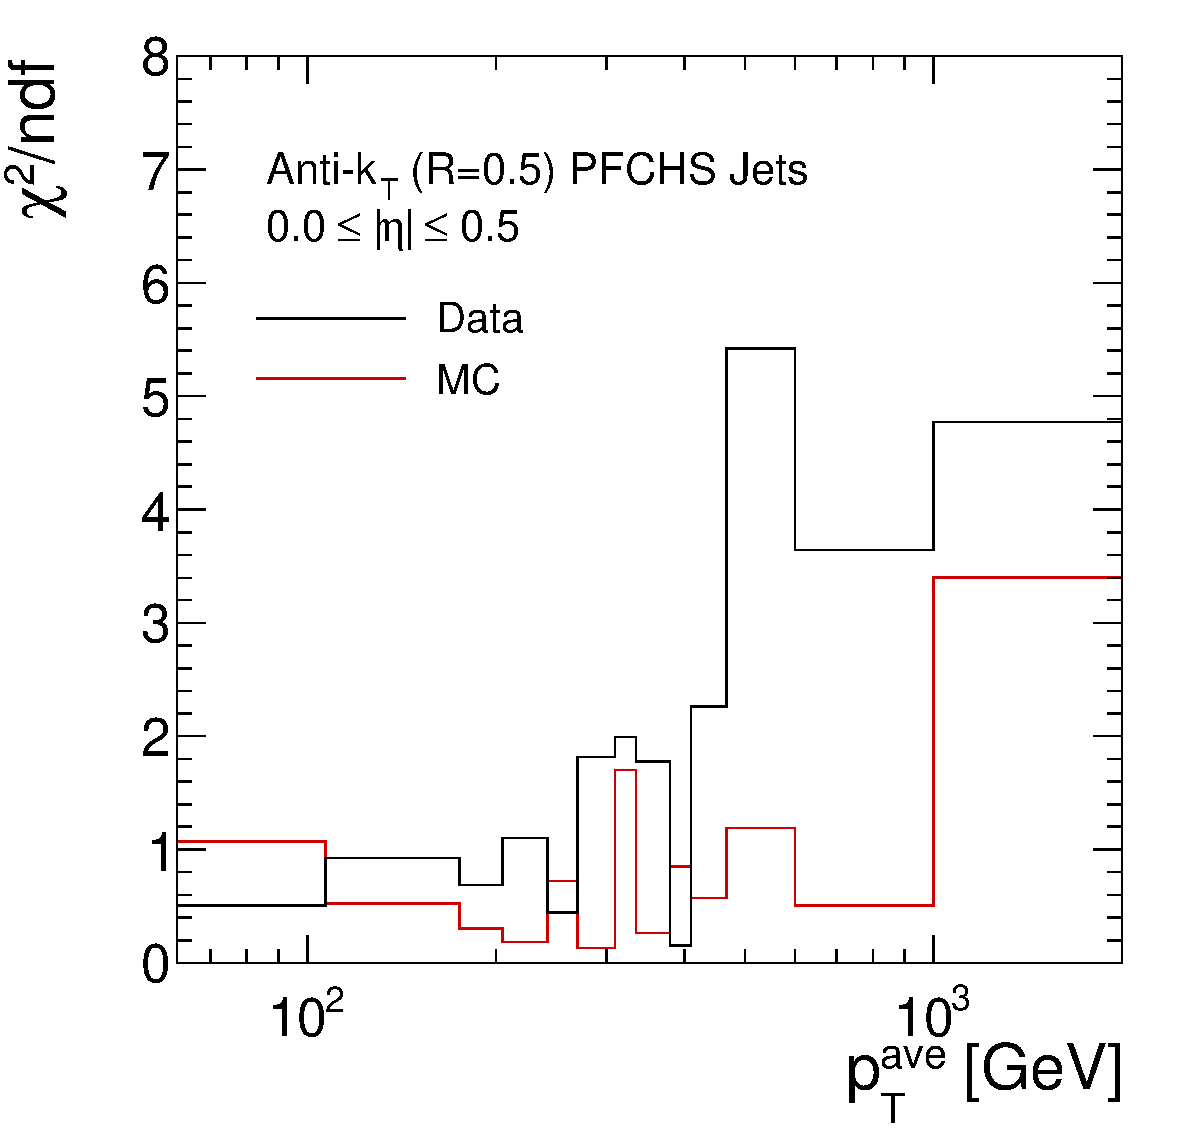
\includegraphics[width=0.49\textwidth]{figures/GoodnessOfFit_Eta0_final_nominal_v4.pdf} &
                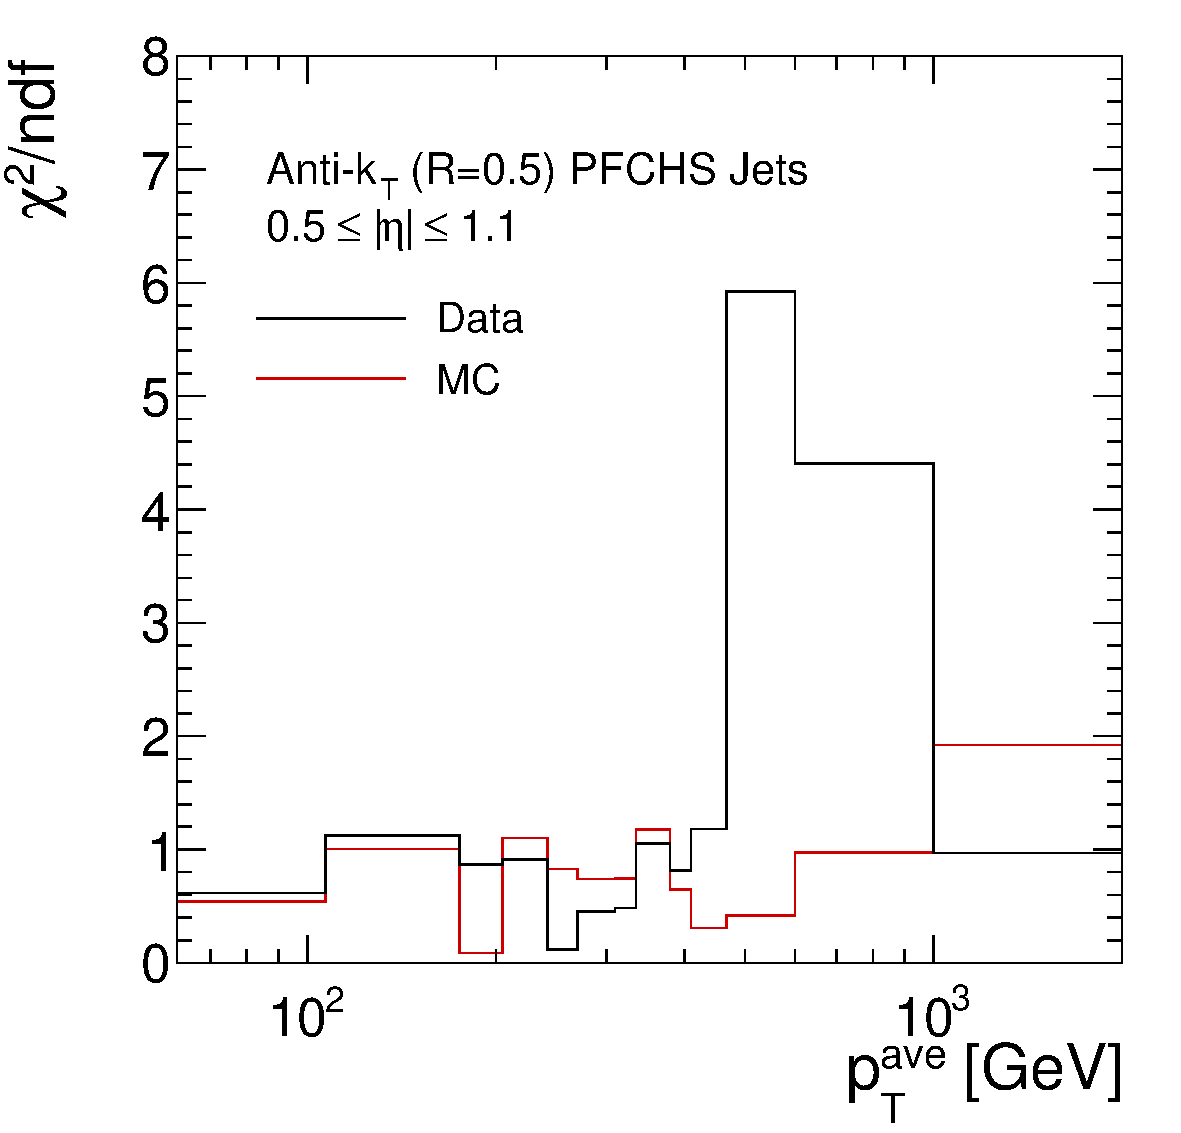
\includegraphics[width=0.49\textwidth]{figures/GoodnessOfFit_Eta1_final_nominal_v4.pdf} \\
 %               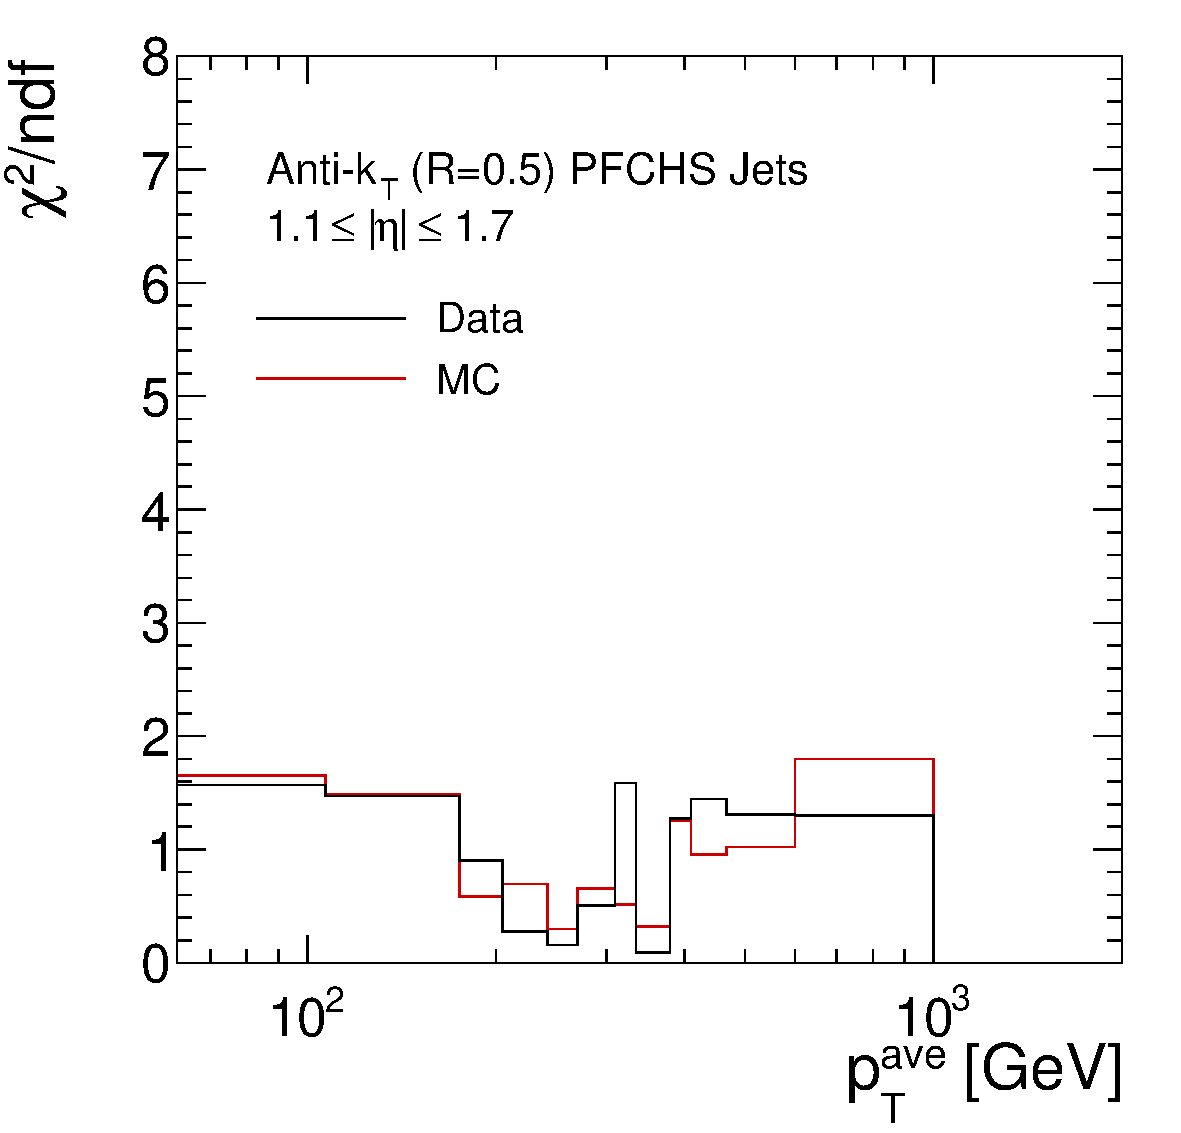
\includegraphics[width=0.49\textwidth]{figures/GoodnessOfFit_Eta2_final_nominal_v4.pdf} &
 %               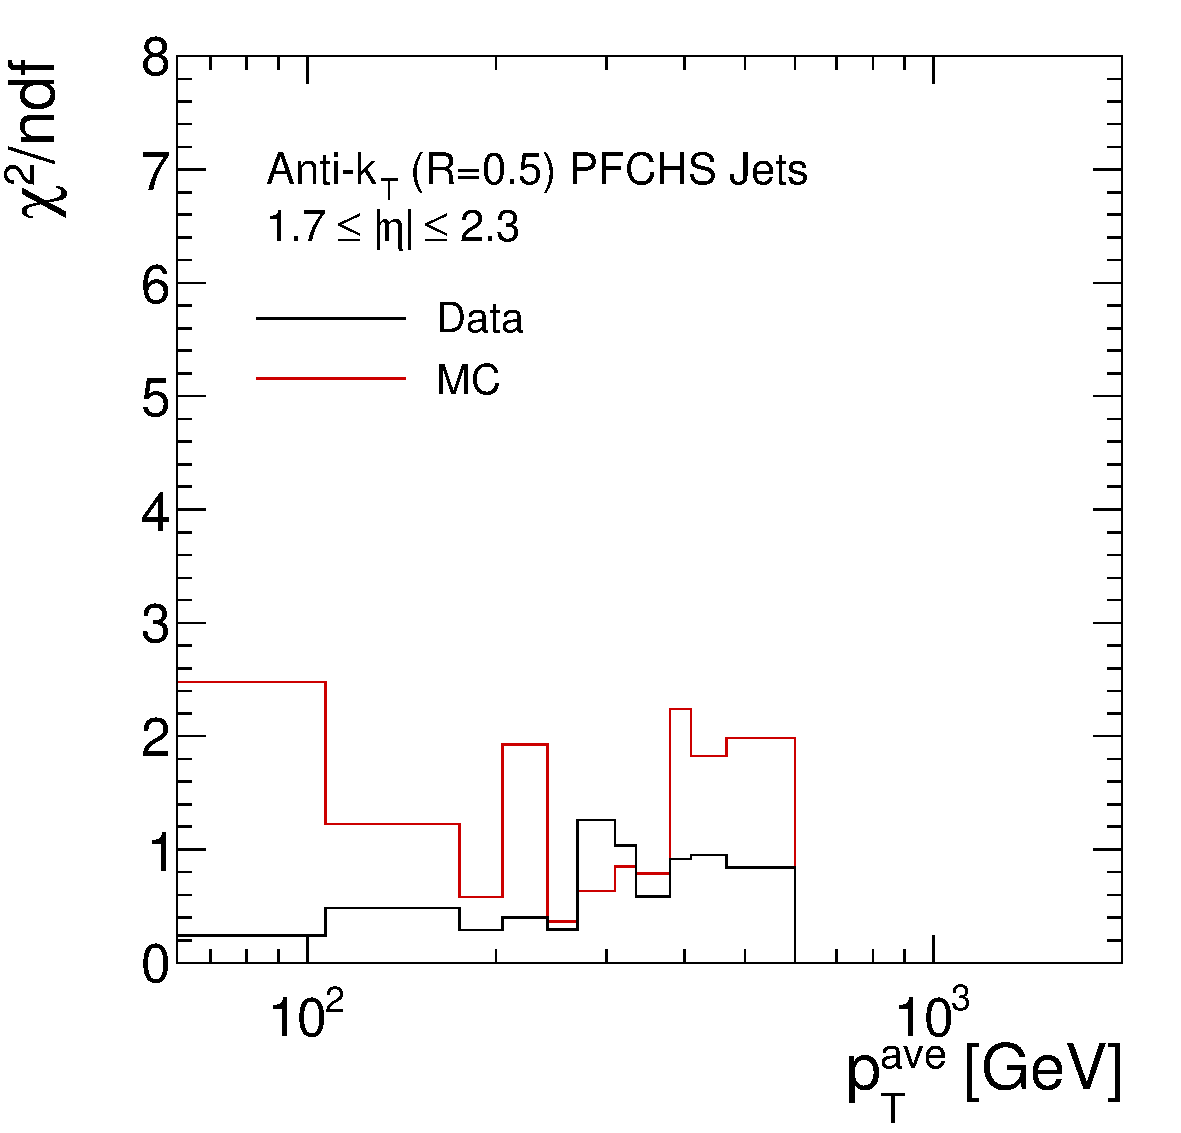
\includegraphics[width=0.49\textwidth]{figures/GoodnessOfFit_Eta3_final_nominal_v4.pdf} \\
 %               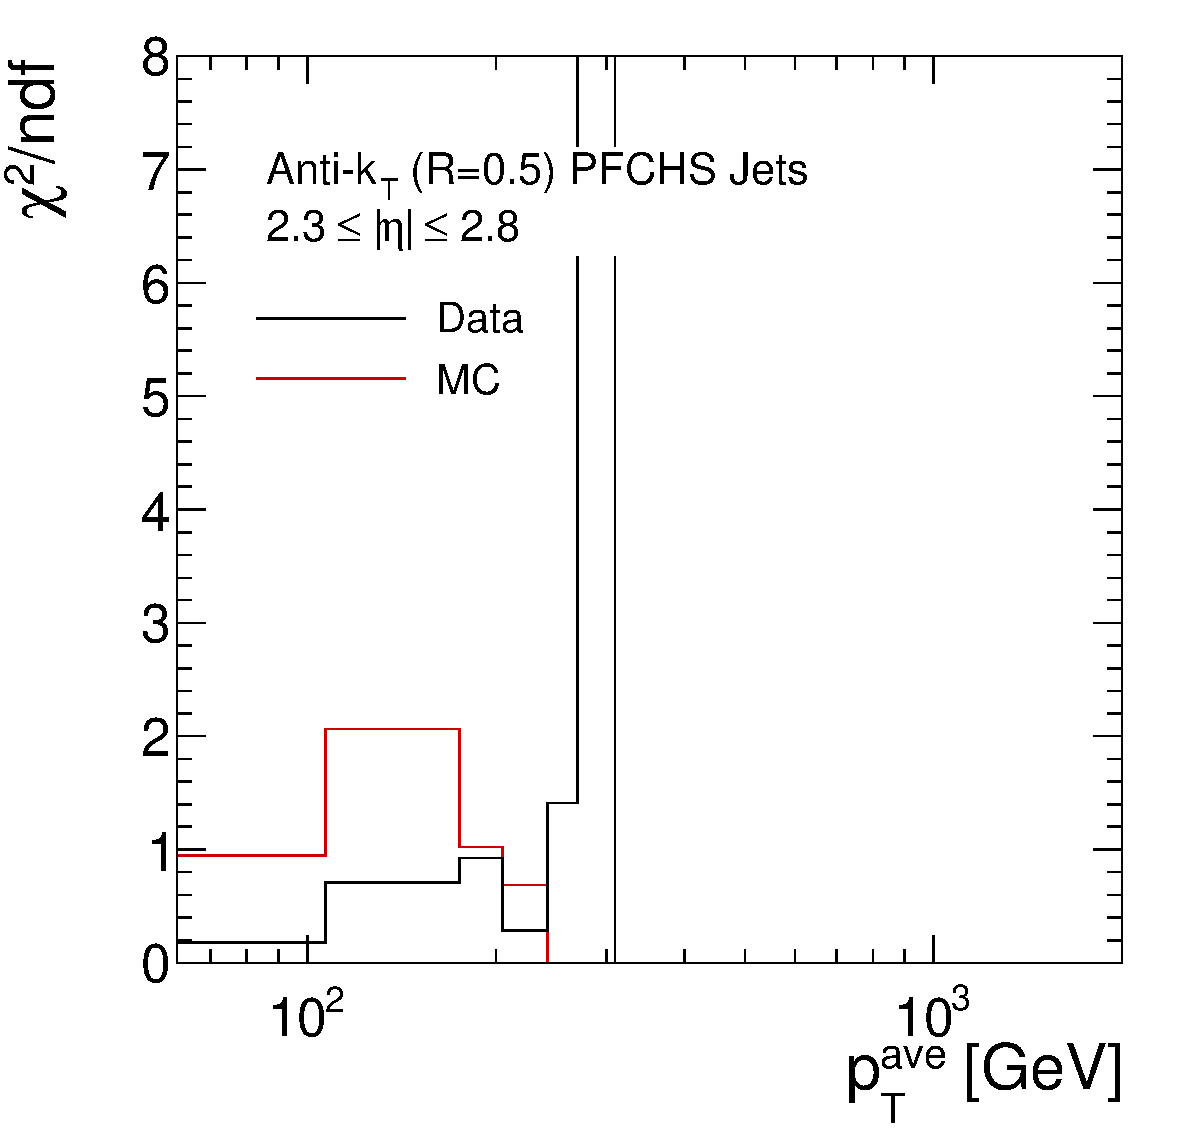
\includegraphics[width=0.49\textwidth]{figures/GoodnessOfFit_Eta4_final_nominal_v4.pdf}
  \end{tabular}
  \caption{Goodness-of-fit test for the extrapolation fits in data and simulation in the two central $|\eta|$ regions as function of $\pt^\mathrm{ave}$.}
  \label{fig:goodness-of-fit}
\end{figure}
In Fig.~\ref{fig:goodness-of-fit}, an overview of a goodness-of-fit test is shown for the extrapolation fits in data and simulation. The resulting values for $\chi^2$ over the number of degrees of freedom are shown as function of $\pt^\mathrm{ave}$ exemplary for the two central $|\eta|$ intervals. This is expected to be distributed around 1. Consequently, the fit quality is in general quite good but worsens for larger $\pt^\mathrm{ave}$ values. Since especially for higher $\pt^\mathrm{ave}$ intervals in the central $|\eta|$ regions, the statistical uncertainty is rather low, the fit is very sensitive to even small deviations from a linear behaviour which results in a minor fit quality. However, a possible non-linearity is considered in the systematic uncertainties of the measurement, as discussed in Section~\ref{sec:jer_syst_unc}.

\subsection{Correction for Particle-Level Imbalance}
\label{subsec:jer_corrections_pli}
In addition to an imbalance in dijet events caused by the presence of additional jets, an imbalance in the dijet system at particle level can also arise for instance from out-of-cone showering. This additional imbalance contribution is referred to as \textit{particle-level imbalance} (PLI) and estimated from simulation. \\
The contribution arising from the particle-level imbalance is estimated from the dijet asymmetry defined at generator level. This is defined equivalently to the asymmetry at detector level but based on generator-level jet quantities as
\begin{equation}
  \mathrm{A^{gen}} = \frac{p_\mathrm{T,1}^\mathrm{gen} - p_\mathrm{T,2}^\mathrm{gen}}{p_\mathrm{T,1}^\mathrm{gen} + p_\mathrm{T,2}^\mathrm{gen}} 
 \end{equation}
with $p_\mathrm{T,1}^\mathrm{gen}$ and $p_\mathrm{T,2}^\mathrm{gen}$ referring to the momenta of the two leading generated jets. This distribution is affected by additional parton radiation as well. Thus, the procedure to obtain $\sigma^\mathrm{gen}_\mathrm{A}(\alpha_\mathrm{max} \rightarrow 0)$ is the same as for the asymmetry at detector level. The generator asymmetry is calculated in the same ($\pt^\mathrm{ave}$, $|\eta|$, $\alpha$)-intervals as the detector-level asymmetry in order to derive the size of the particle-level imbalance for exactly the same events. The asymmetry width of the generator asymmetry is also calculated as $\mathrm{RMS}_{98.5\%}$. In order to obtain the values of $\sigma^\mathrm{gen}_\mathrm{A}$ for zero additional jet activity, the analogue extrapolation procedure is performed, as described in Sec.~\ref{subsec:jer_corrections_alpha}. Some example extrapolations are illustrated in Fig.~\ref{fig:extrapol_gen}. 
\begin{figure}[!tp]
  \centering
  \begin{tabular}{cc}
                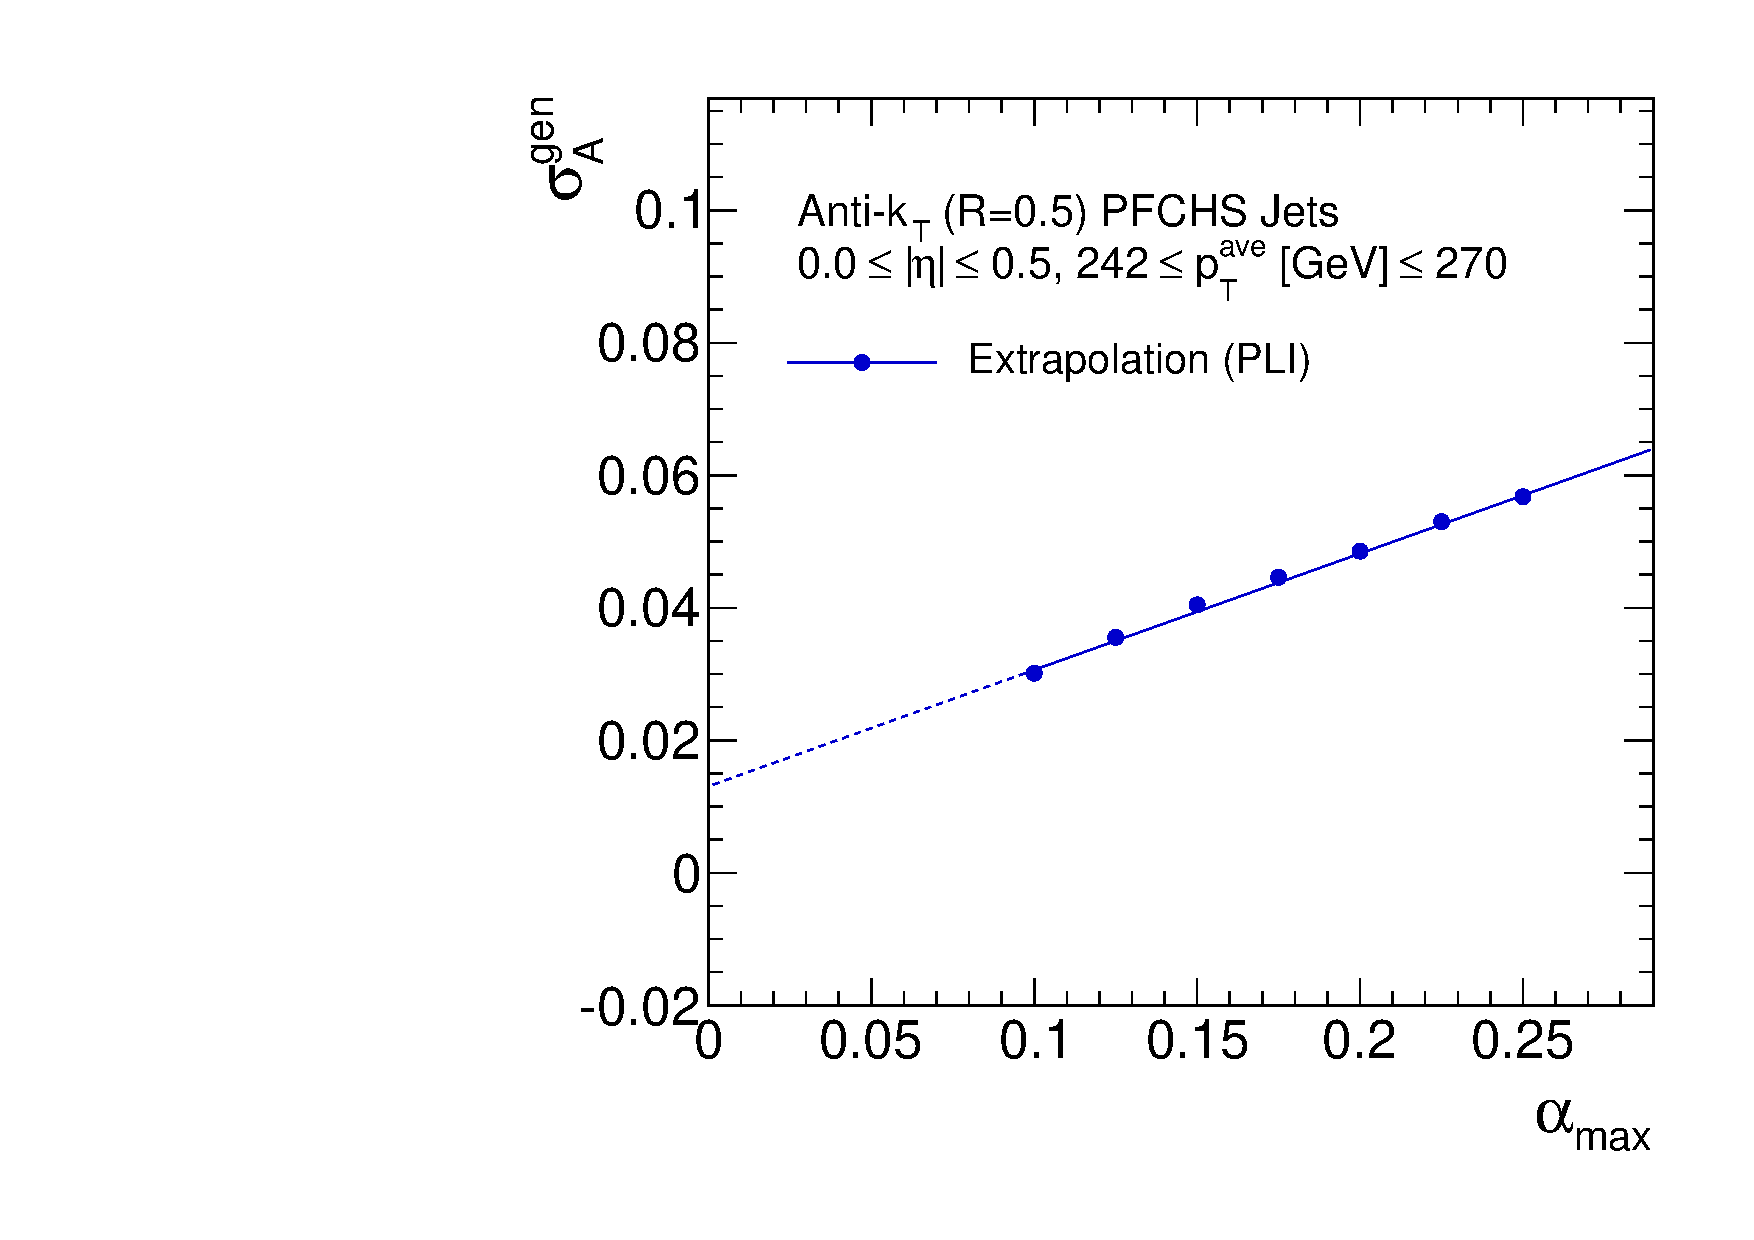
\includegraphics[width=0.49\textwidth]{figures/Extrapol_Eta0_pt4_gen_final_nominal_v4b.pdf} &
                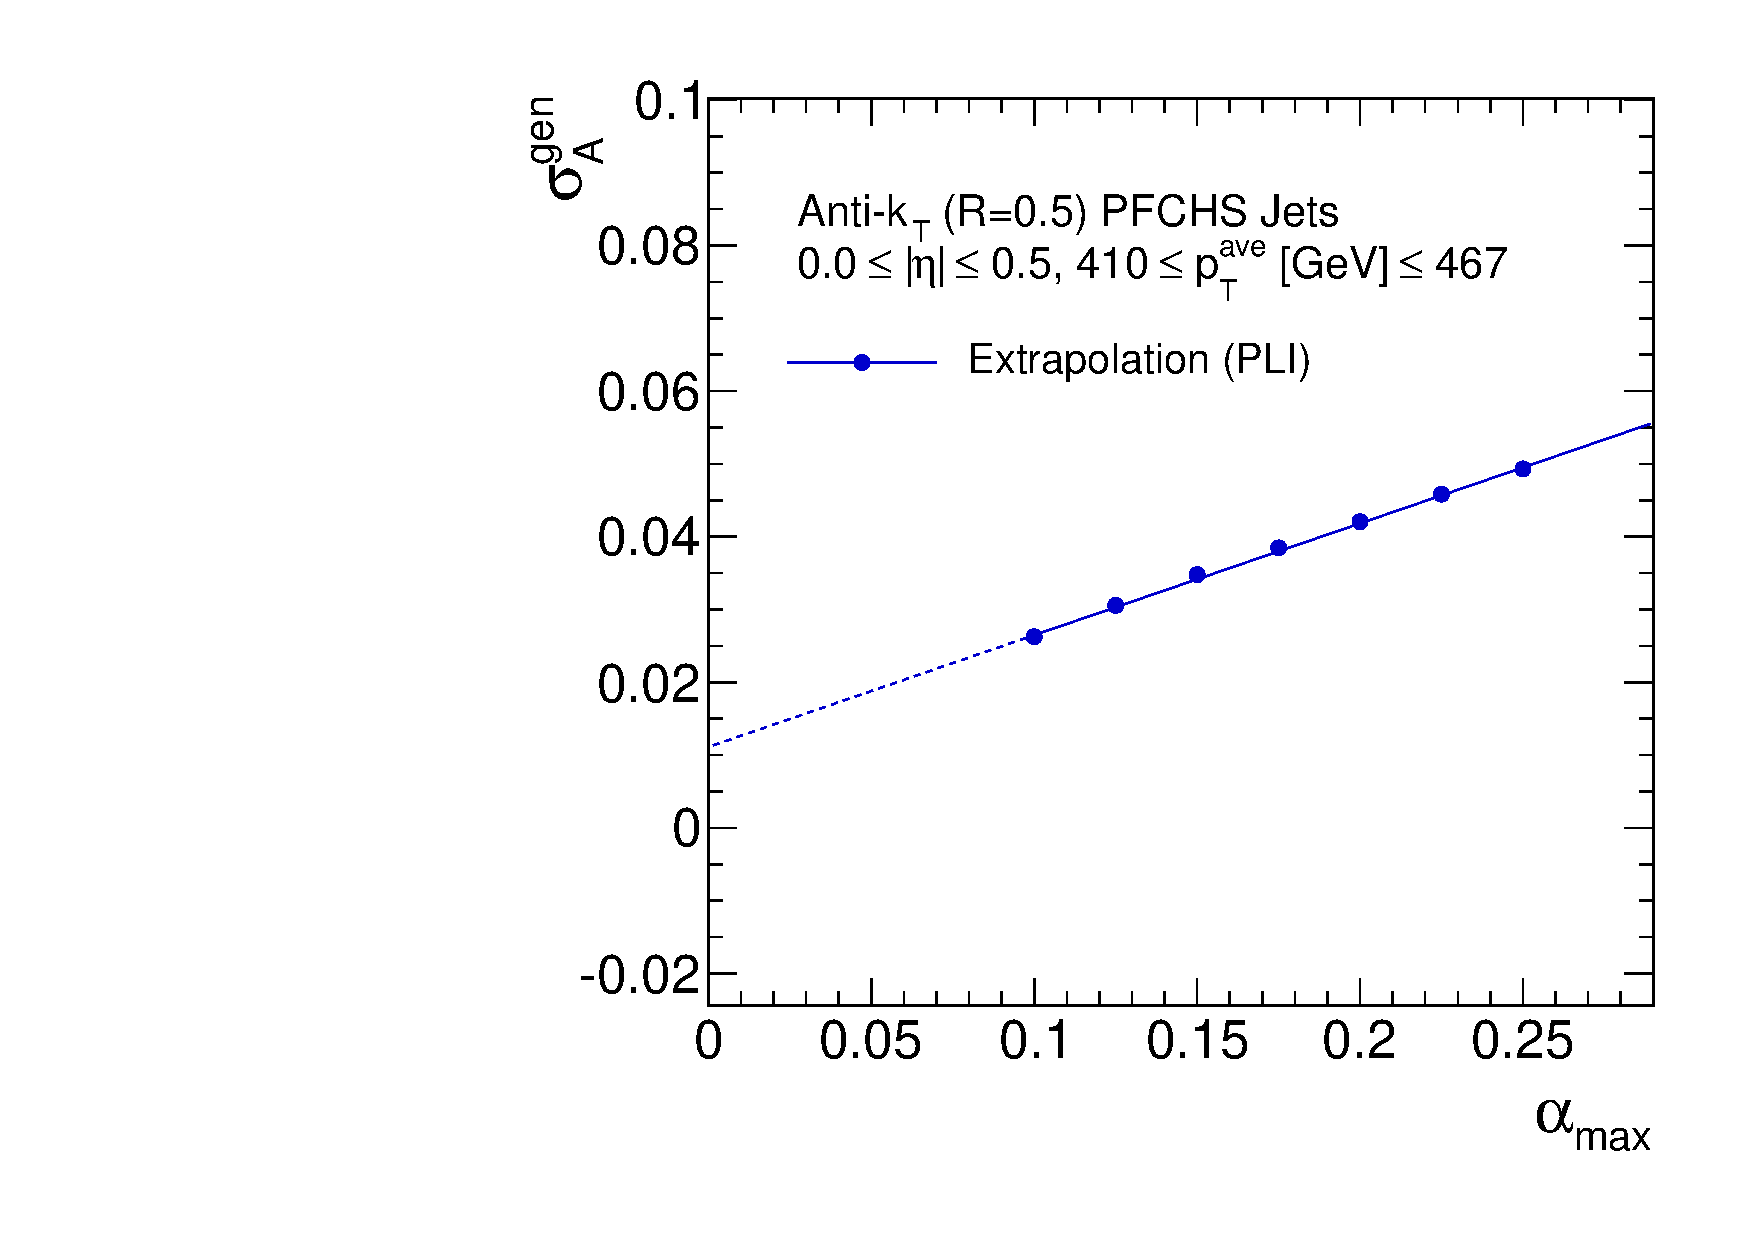
\includegraphics[width=0.49\textwidth]{figures/Extrapol_Eta0_pt9_gen_final_nominal_v4b.pdf}
  \end{tabular}
  \caption{Two example extrapolations of measured values for $\sigma^\mathrm{gen}_\mathrm{A}$ in simulation to determine the contribution from PLI.}
  \label{fig:extrapol_gen}
\end{figure}
\\
Finally, the results of the extrapolated values for $\sigma^\mathrm{gen}_\mathrm{A}$ can be used to quantify the size of the particle-level imbalance. This is given by
 \begin{equation}
 \label{eq:pli}
 \sigma_\mathrm{PLI} = \sqrt{2} \cdot \sigma^\mathrm{gen}_\mathrm{A}(\alpha_\mathrm{max} \rightarrow 0) \, .
 \end{equation}

\subsection{Results of the Corrections to the Asymmetry}
\label{subsec:jer_corrections_results} 
The results of the various extrapolation fits to determine $ \sigma_\mathrm{A}(\alpha_\mathrm{max} \rightarrow 0)$ in data and simulation as well as for the particle-level imbalance are shown together in Fig.~\ref{fig:fit-results} as a function of $\pt^\mathrm{ave}$ for the different $|\eta|$ regions. 
\begin{figure}[!htp]
  \centering
  \begin{tabular}{cc}
                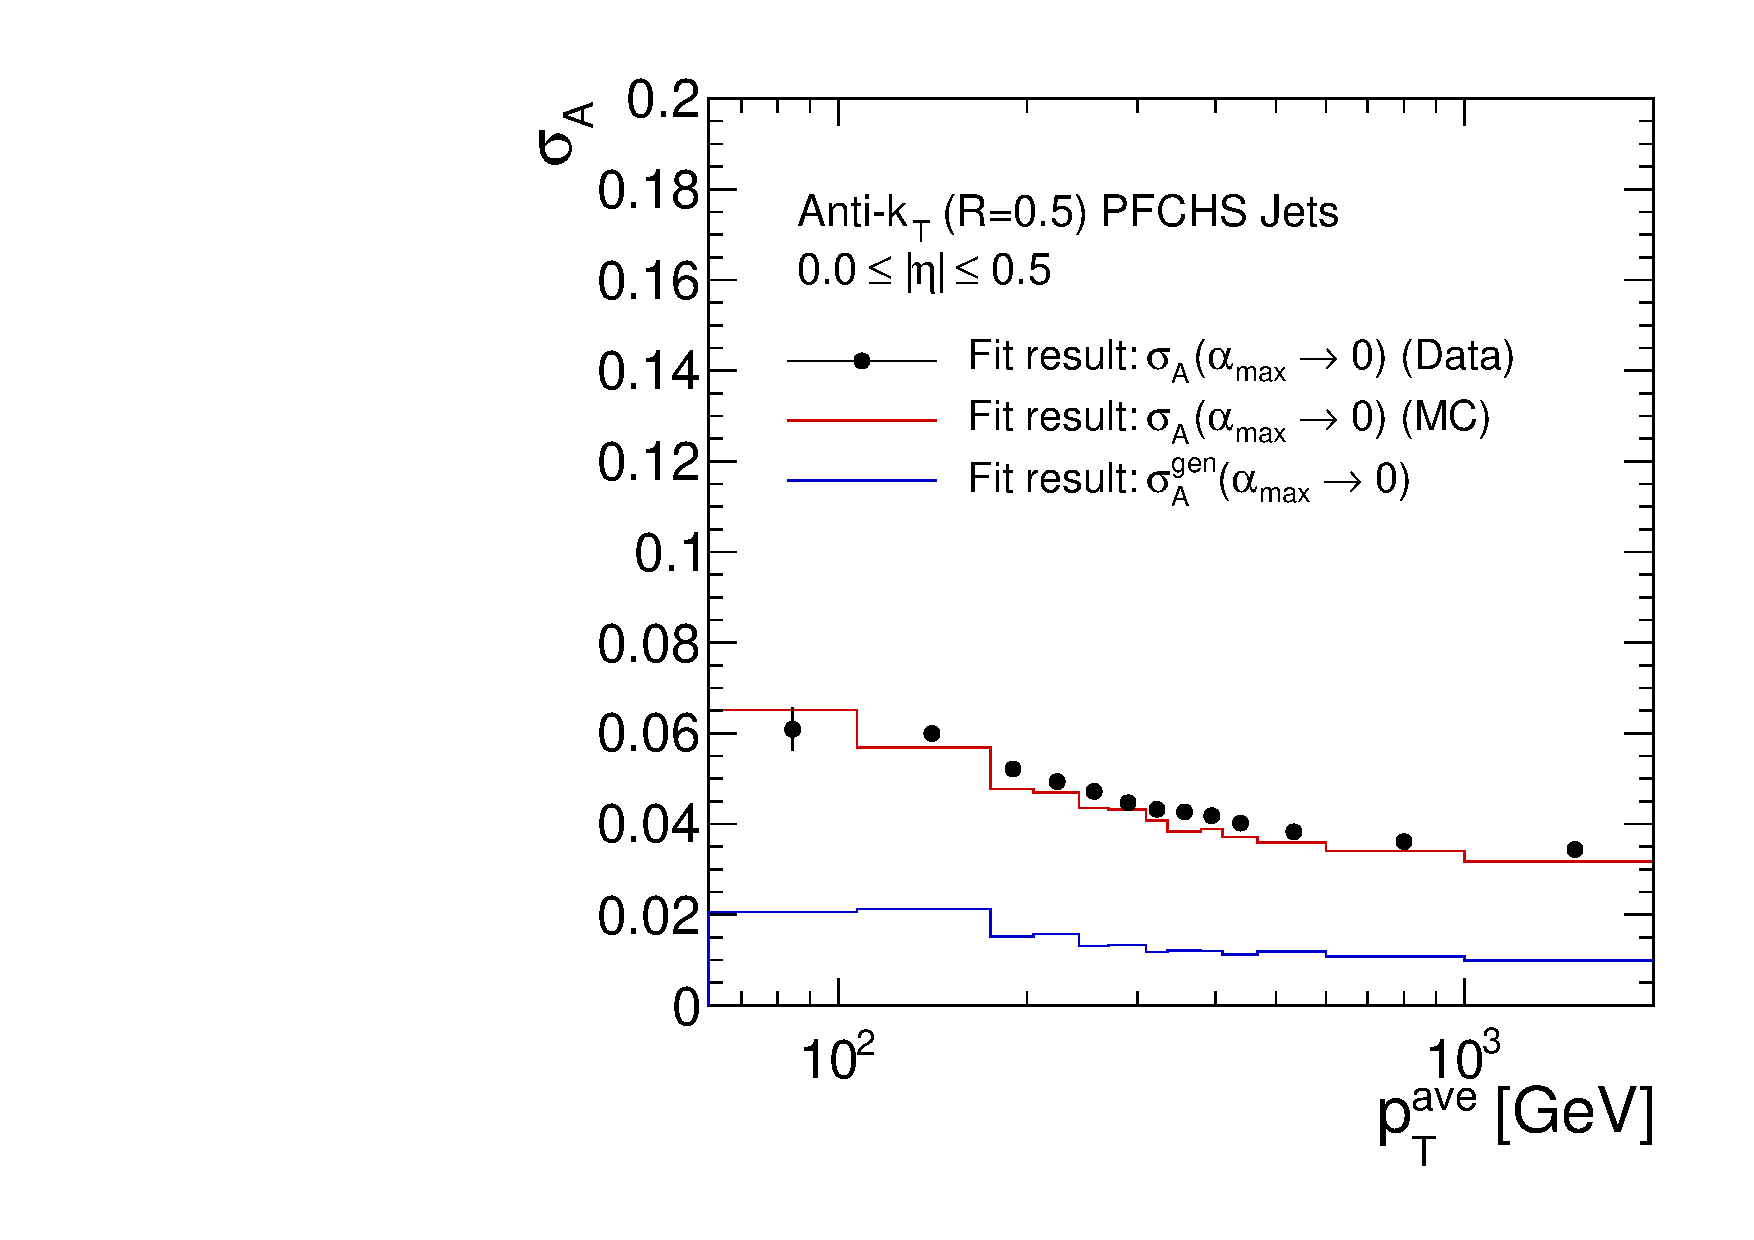
\includegraphics[width=0.49\textwidth]{figures/Extrapol_Eta0_final_nominal_v4b.pdf} &
                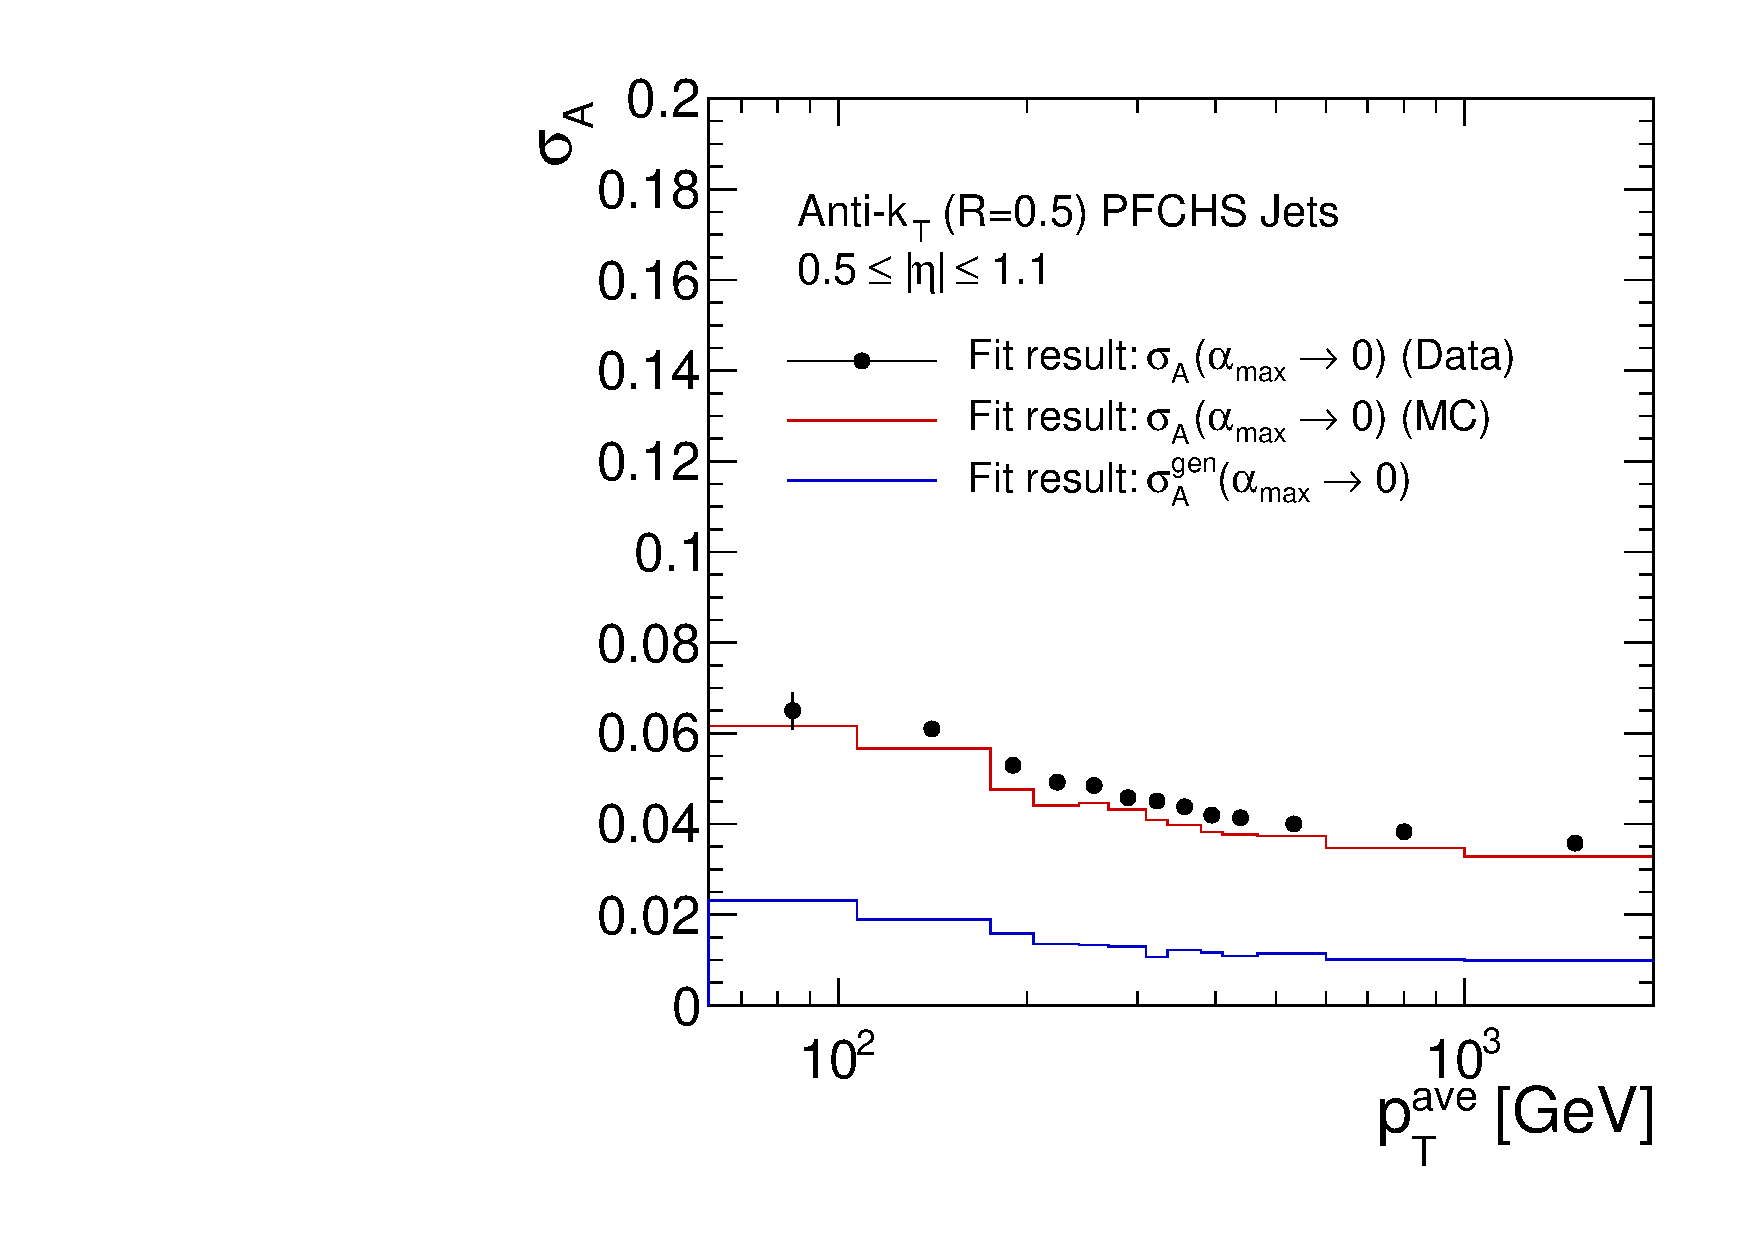
\includegraphics[width=0.49\textwidth]{figures/Extrapol_Eta1_final_nominal_v4b.pdf} \\
  %              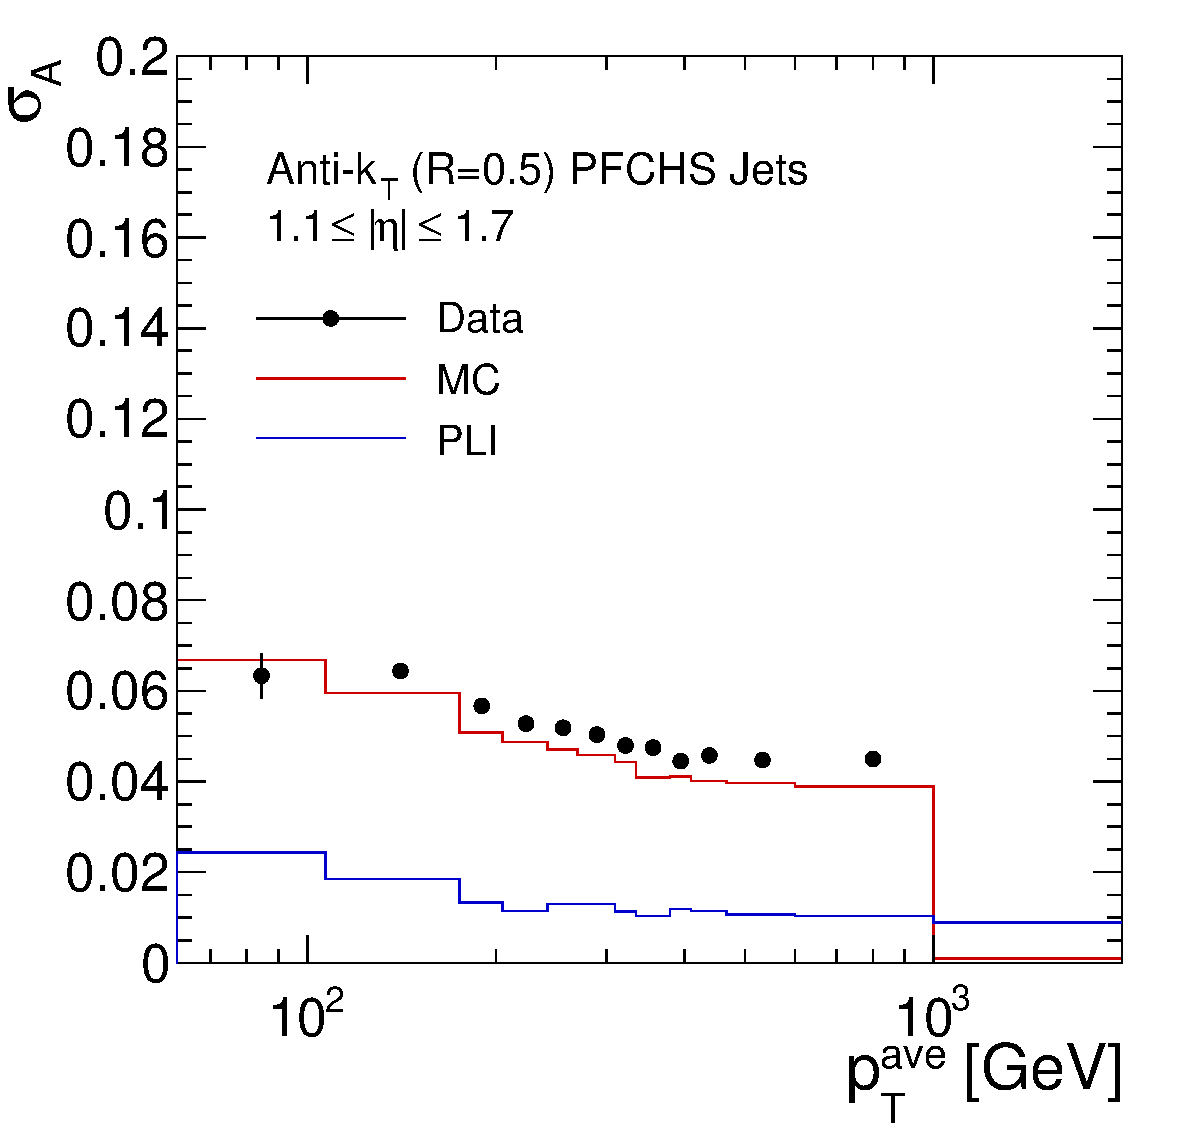
\includegraphics[width=0.49\textwidth]{figures/Extrapol_Eta2_final_nominal_v4.pdf} &
  %              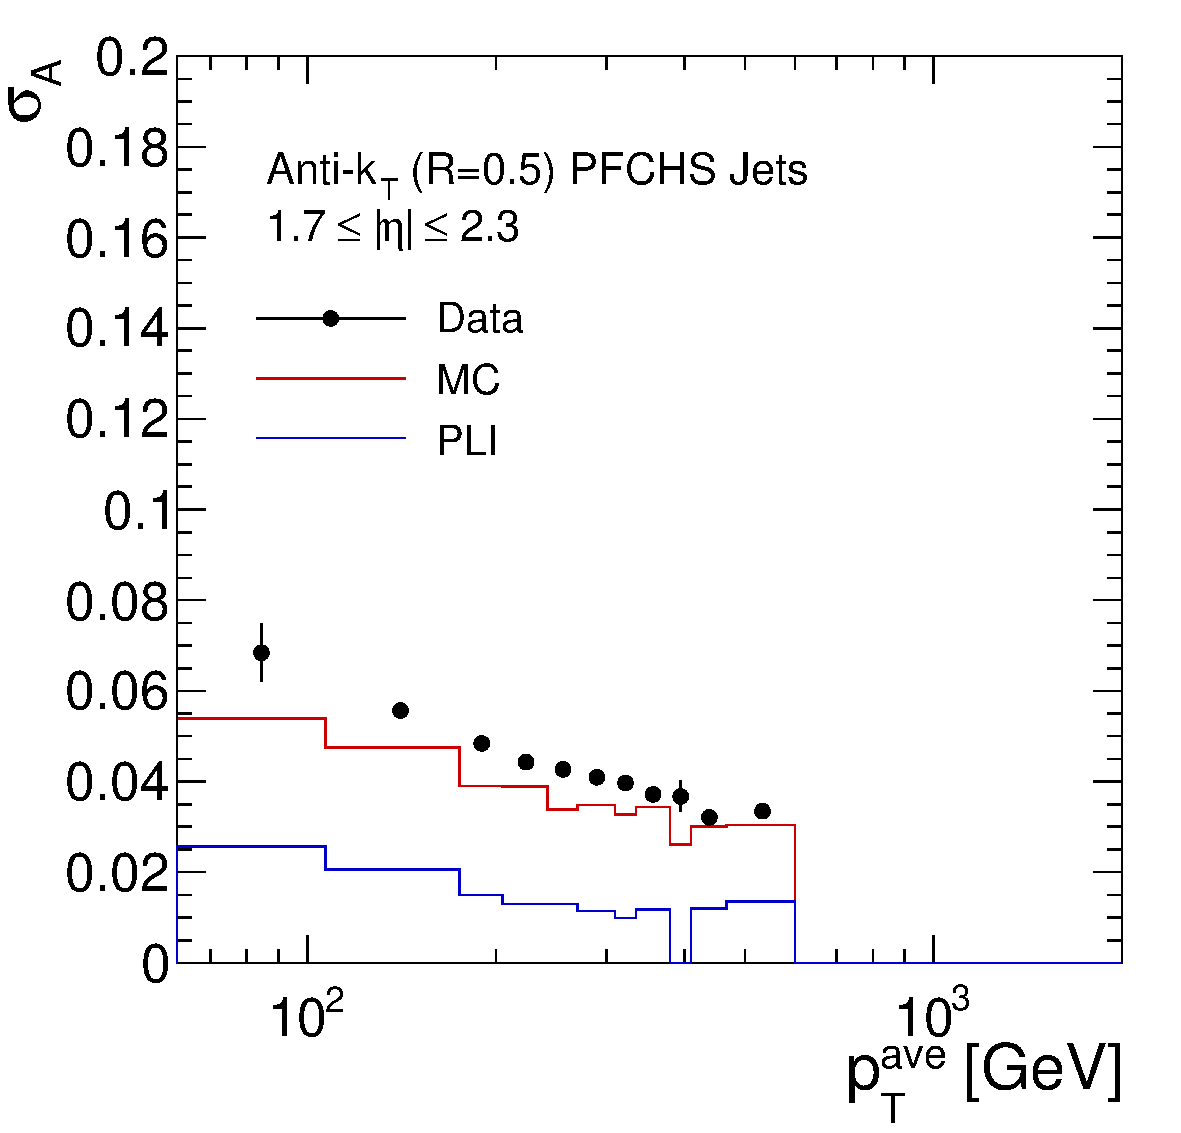
\includegraphics[width=0.49\textwidth]{figures/Extrapol_Eta3_final_nominal_v4.pdf} \\
  %              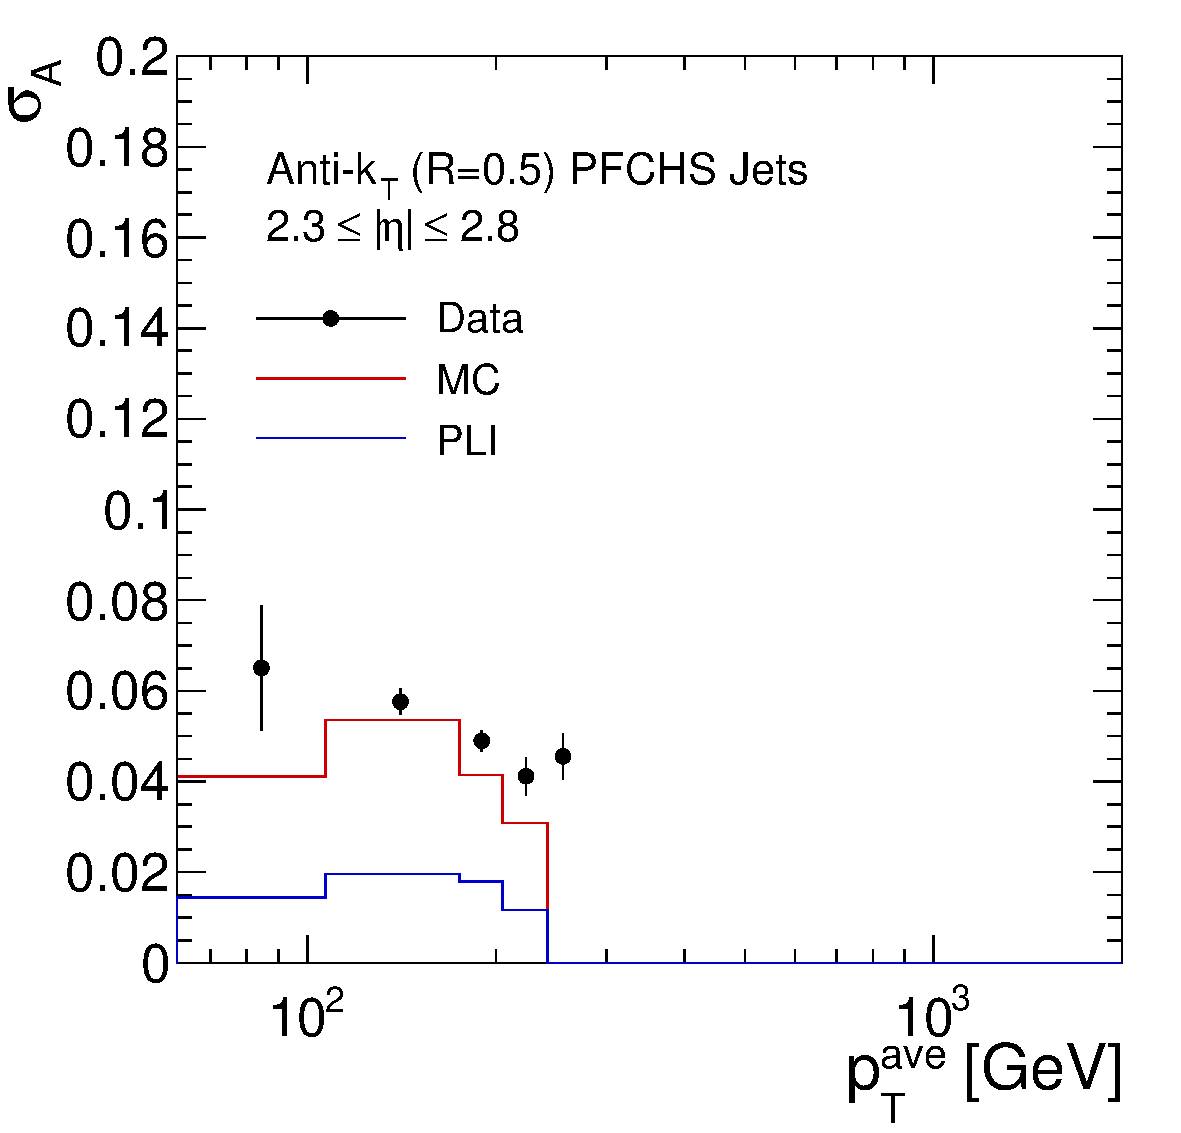
\includegraphics[width=0.49\textwidth]{figures/Extrapol_Eta4_final_nominal_v4.pdf}
  \end{tabular}
  \caption{Results of extrapolation fits in the two central $|\eta|$ regions as a function of $\pt^\mathrm{ave}$ for data (black), simulation (red) and particle-level imbalance (blue).}
  \label{fig:fit-results}
\end{figure}
\\
In order to obtain the jet energy resolution, the results of the extrapolated detector-level asymmetry widths are corrected for the effects from particle-level imbalance. This is done by subtracting the PLI correction in quadrature from the measured $\sigma_\mathrm{A}$ after the correction for additional jet activity 
\begin{equation}
\sigma_\mathrm{JER} =  \sqrt{2} \cdot \sigma_\mathrm{A}(\alpha_\mathrm{max} \rightarrow 0) \ominus \sigma_\mathrm{PLI} \, .
\end{equation}  
The same PLI correction is substracted both from data as well as from simulation results. As can be seen in Fig.~\ref{fig:fit-results}, the correction due to particle-level imbalance is small compared to the measured asymmetry widths. This justifies to take this correction from simulation, also for the data resolution. However, in order to account for a possible imprecise modelling of the particle-level imbalance contribution, a systematic uncertainty will be considered, as discussed in Sec.~\ref{sec:jer_syst_unc}.

\section[Determination of the Data-to-Simulation Ratio]{Determination of the Data-to-Simulation Ratio of the Jet Transverse Momentum Resolution}
\label{sec:jer_ratio_determination}
\begin{figure}[!htp]
  \centering
  \begin{tabular}{cc}
                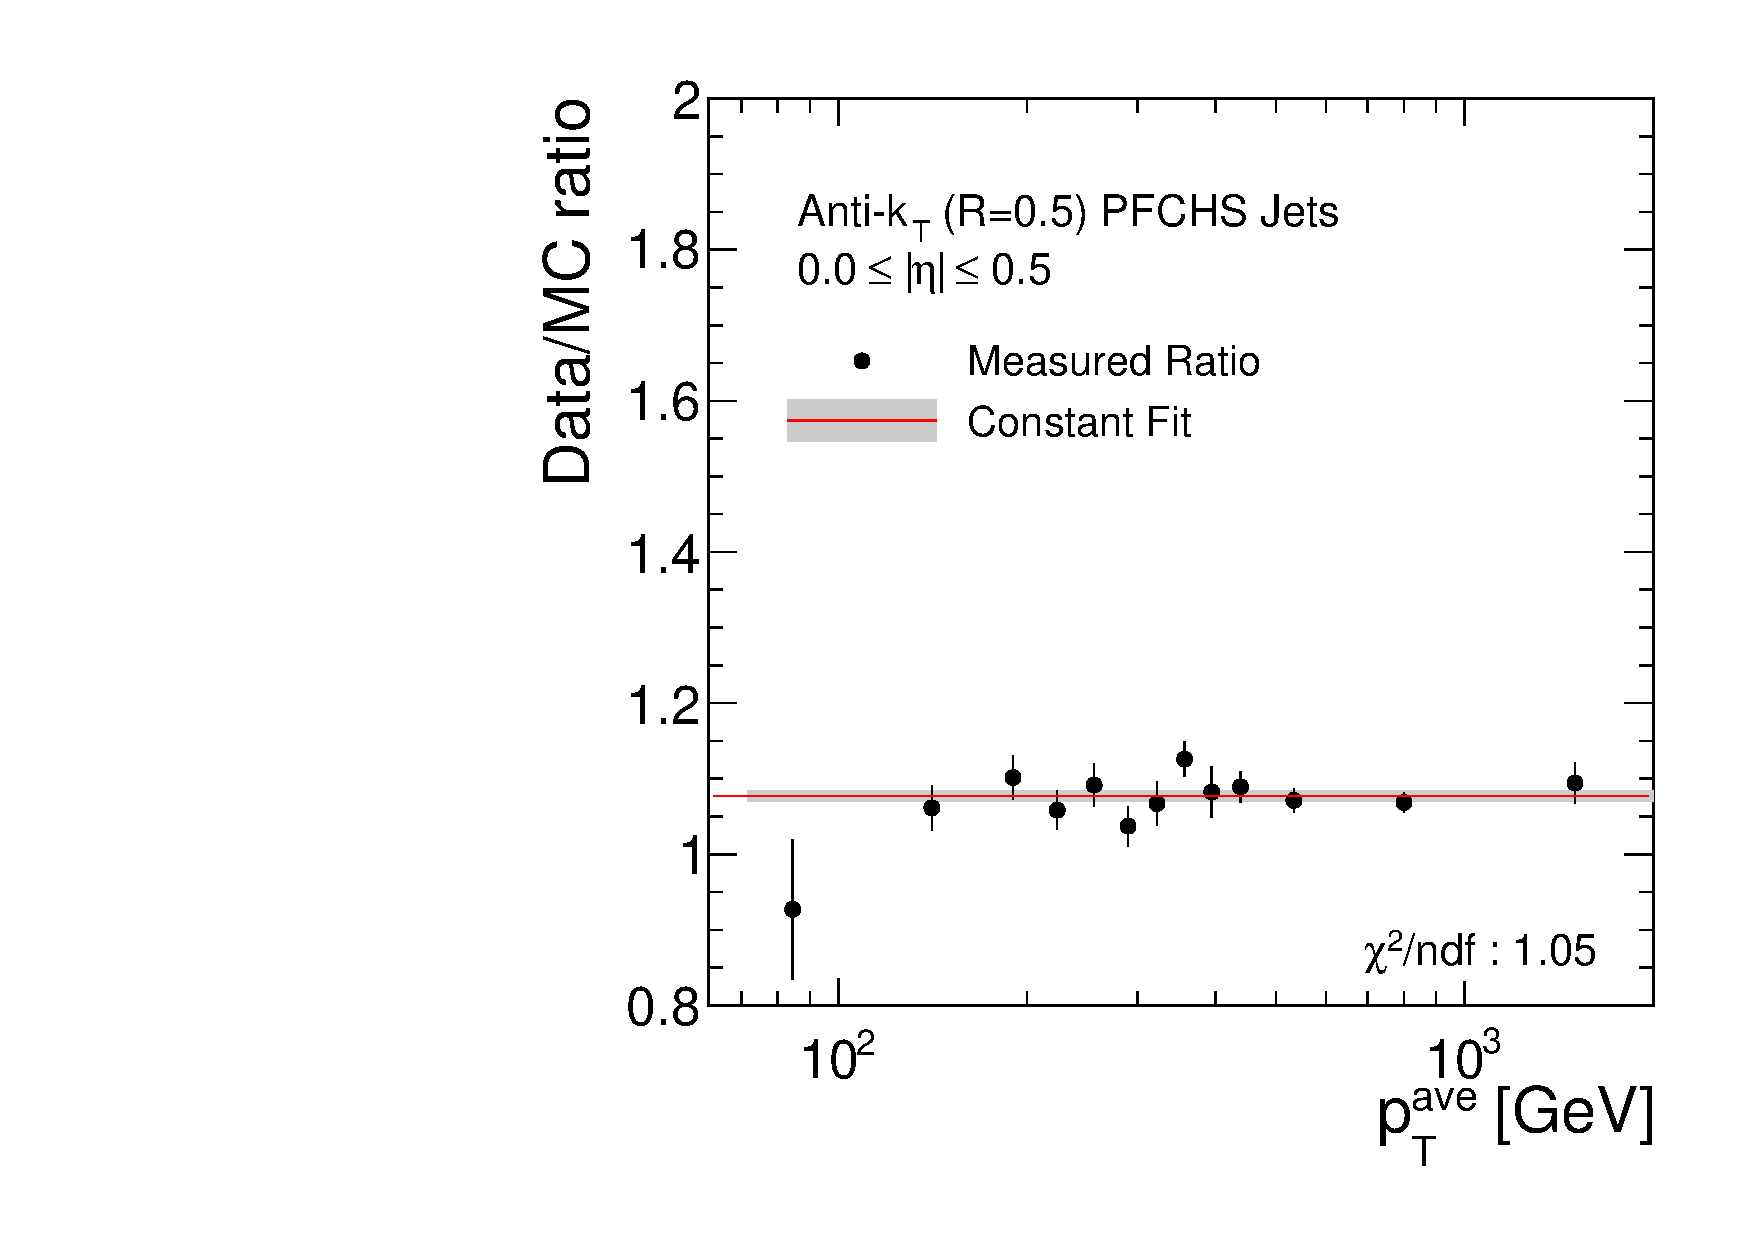
\includegraphics[width=0.49\textwidth]{figures/ExtrapolRatio_Eta0_with_pli_final_nominal_v4b.pdf} &
                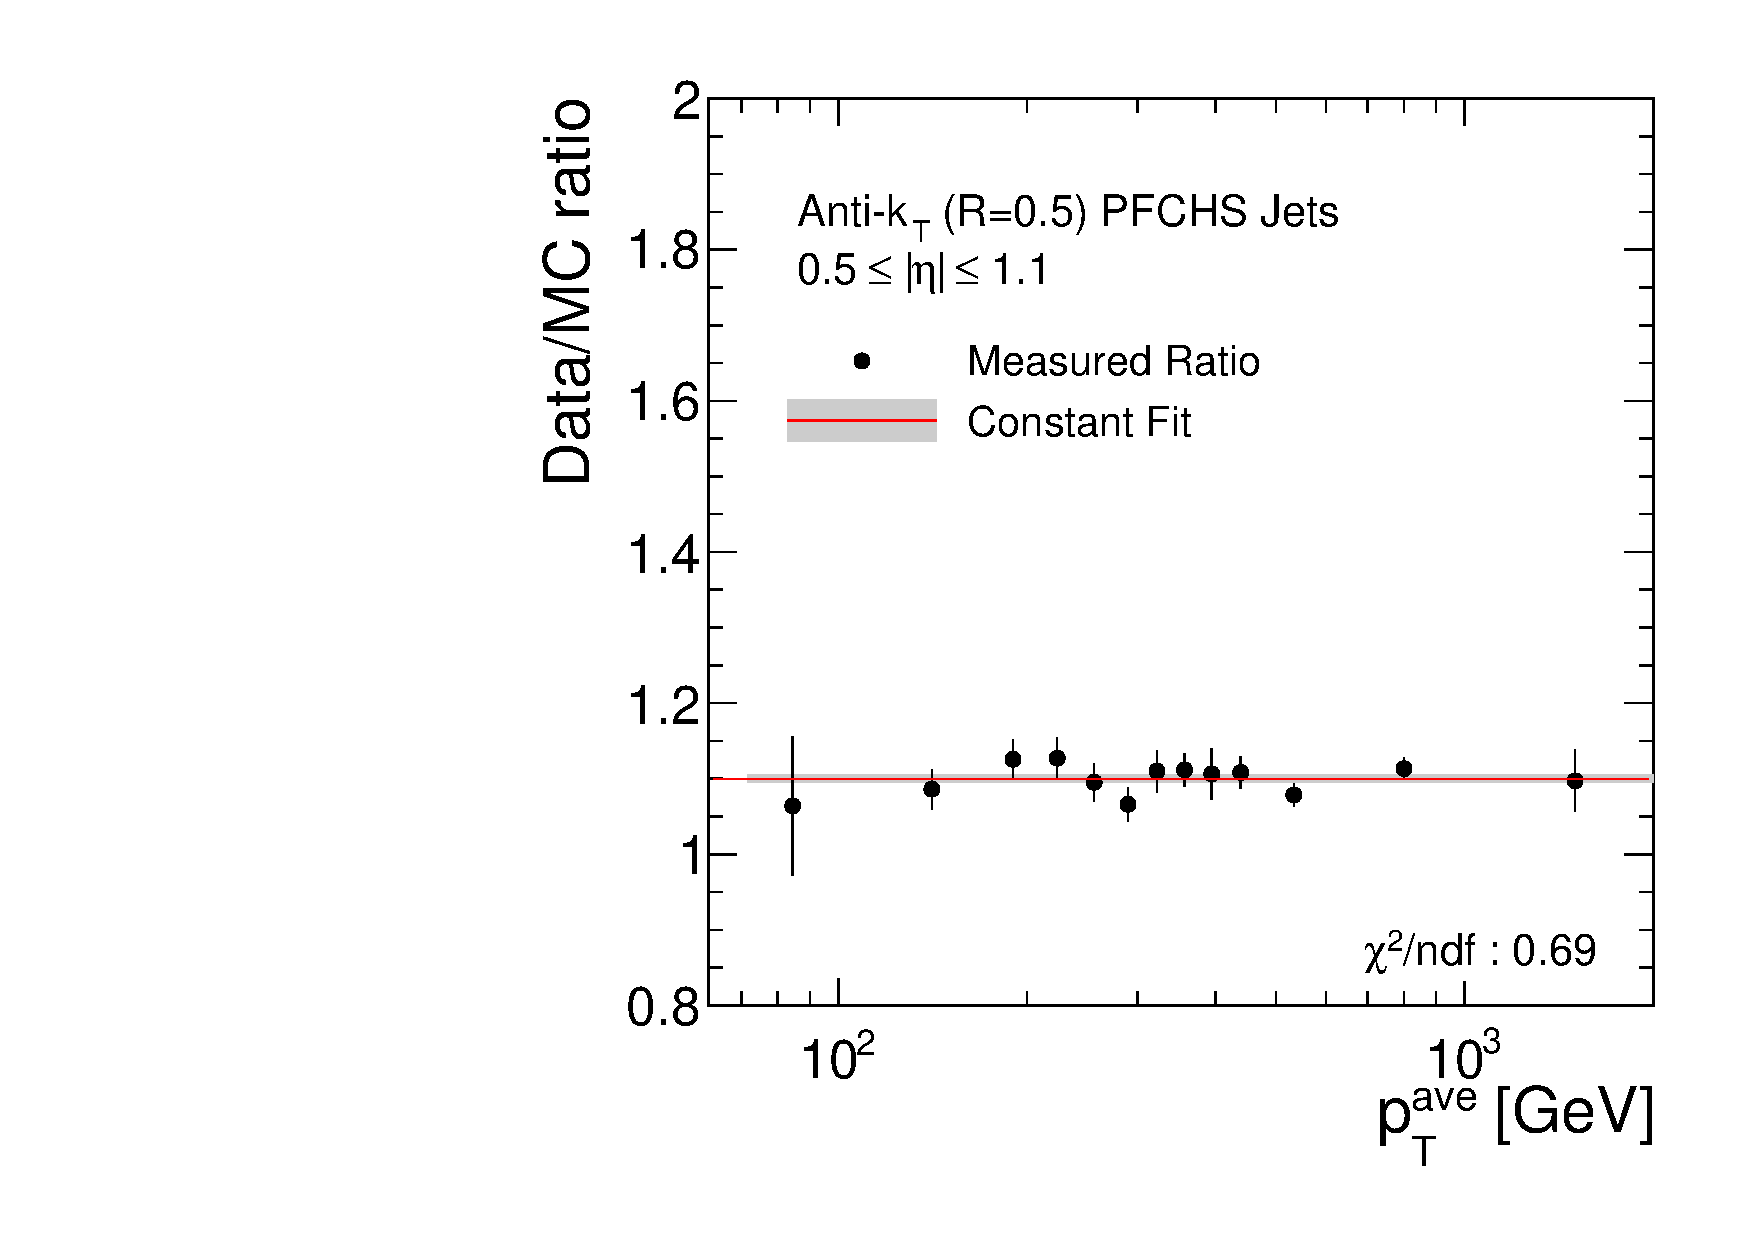
\includegraphics[width=0.49\textwidth]{figures/ExtrapolRatio_Eta1_with_pli_final_nominal_v4b.pdf} \\
                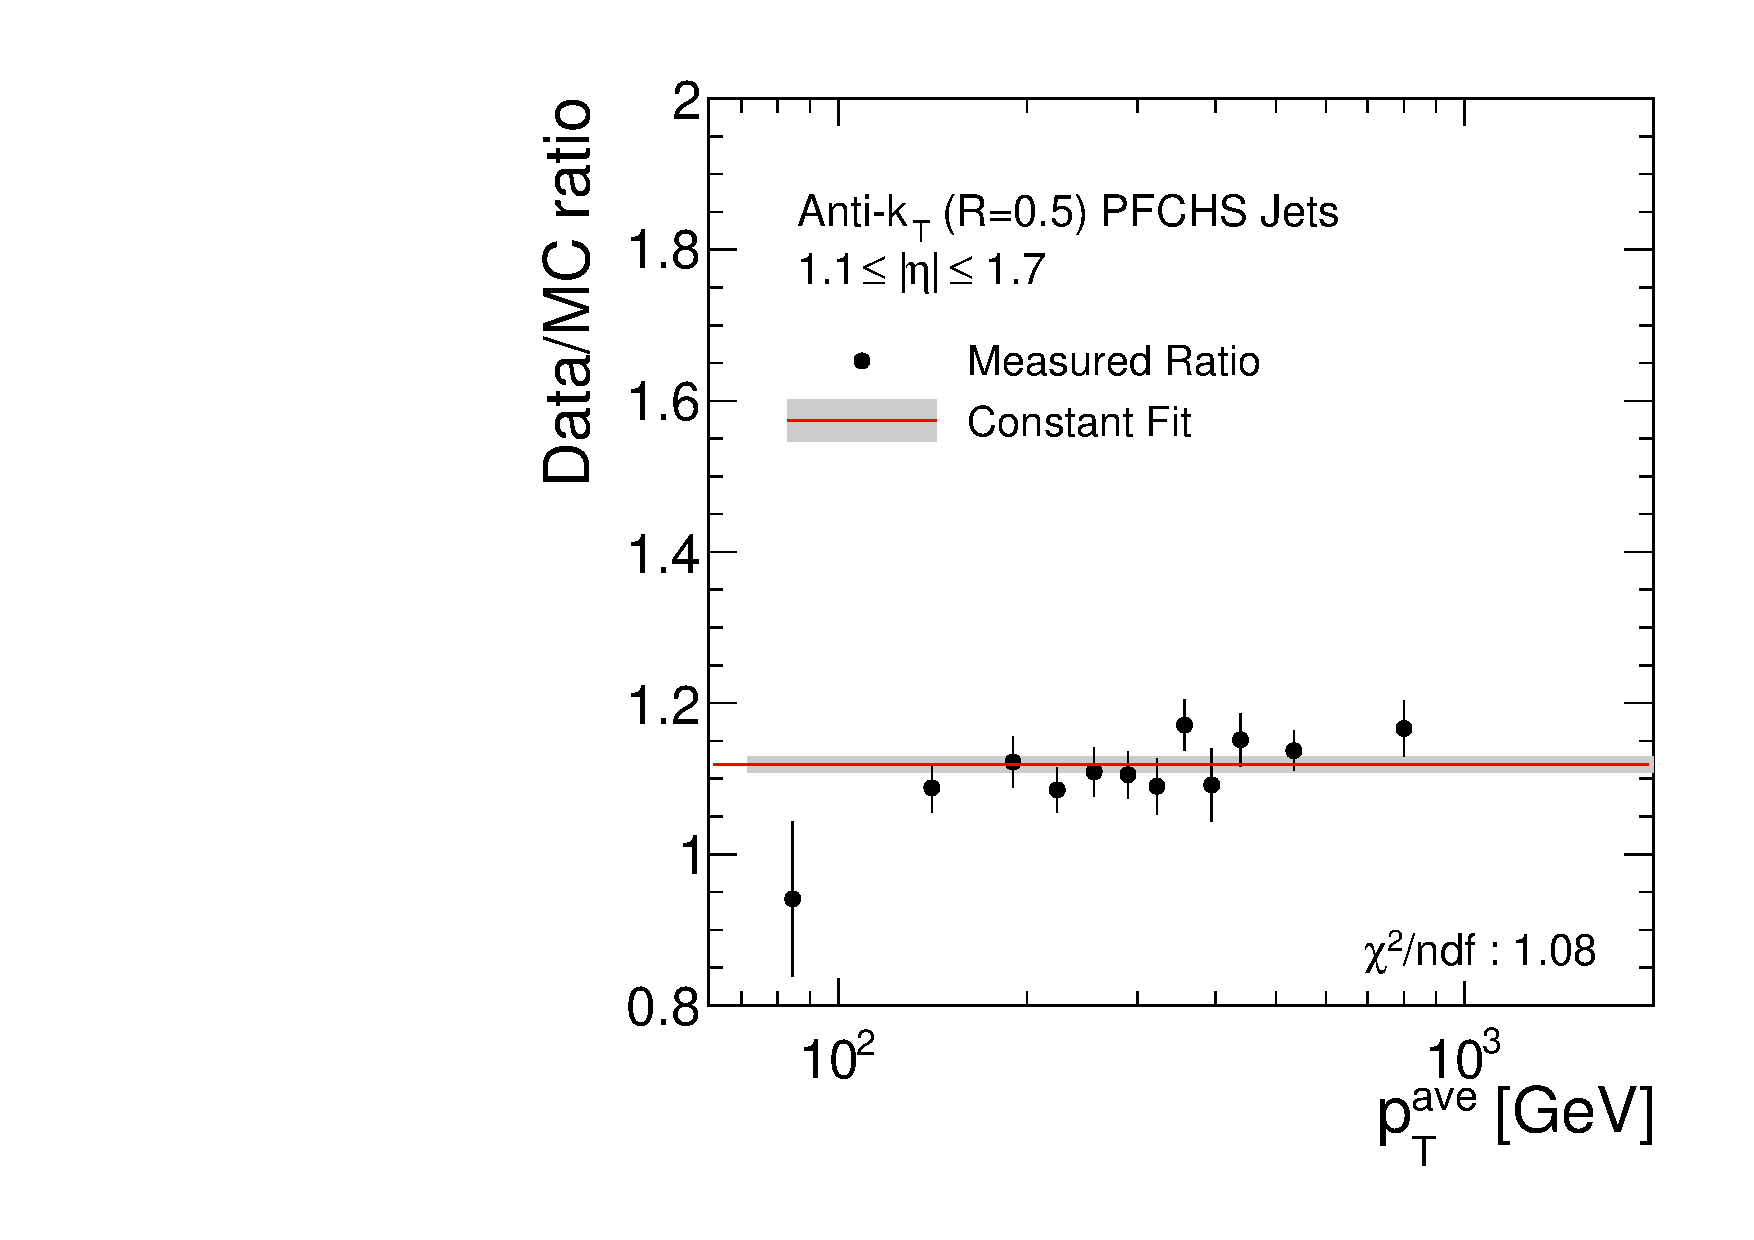
\includegraphics[width=0.49\textwidth]{figures/ExtrapolRatio_Eta2_with_pli_final_nominal_v4b.pdf} &
                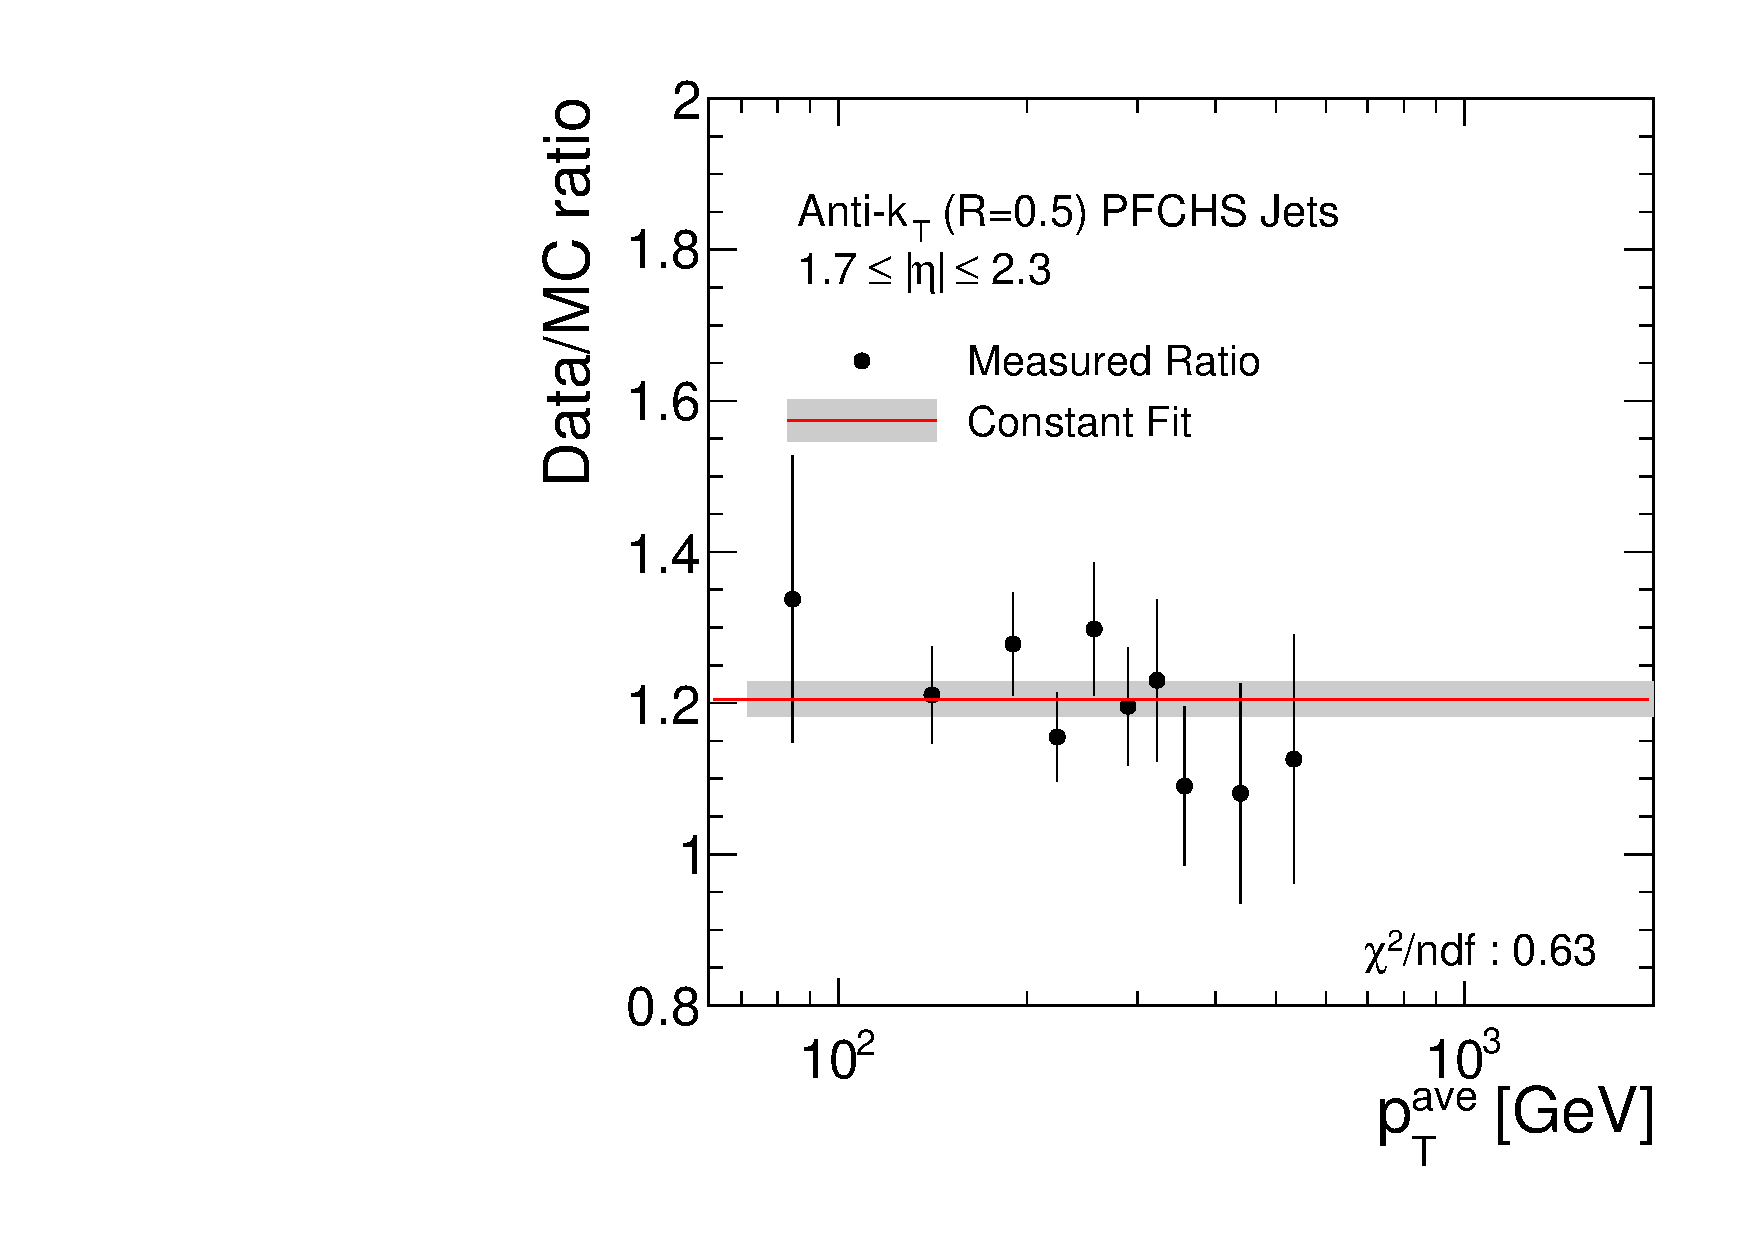
\includegraphics[width=0.49\textwidth]{figures/ExtrapolRatio_Eta3_with_pli_final_nominal_v4b.pdf} \\
                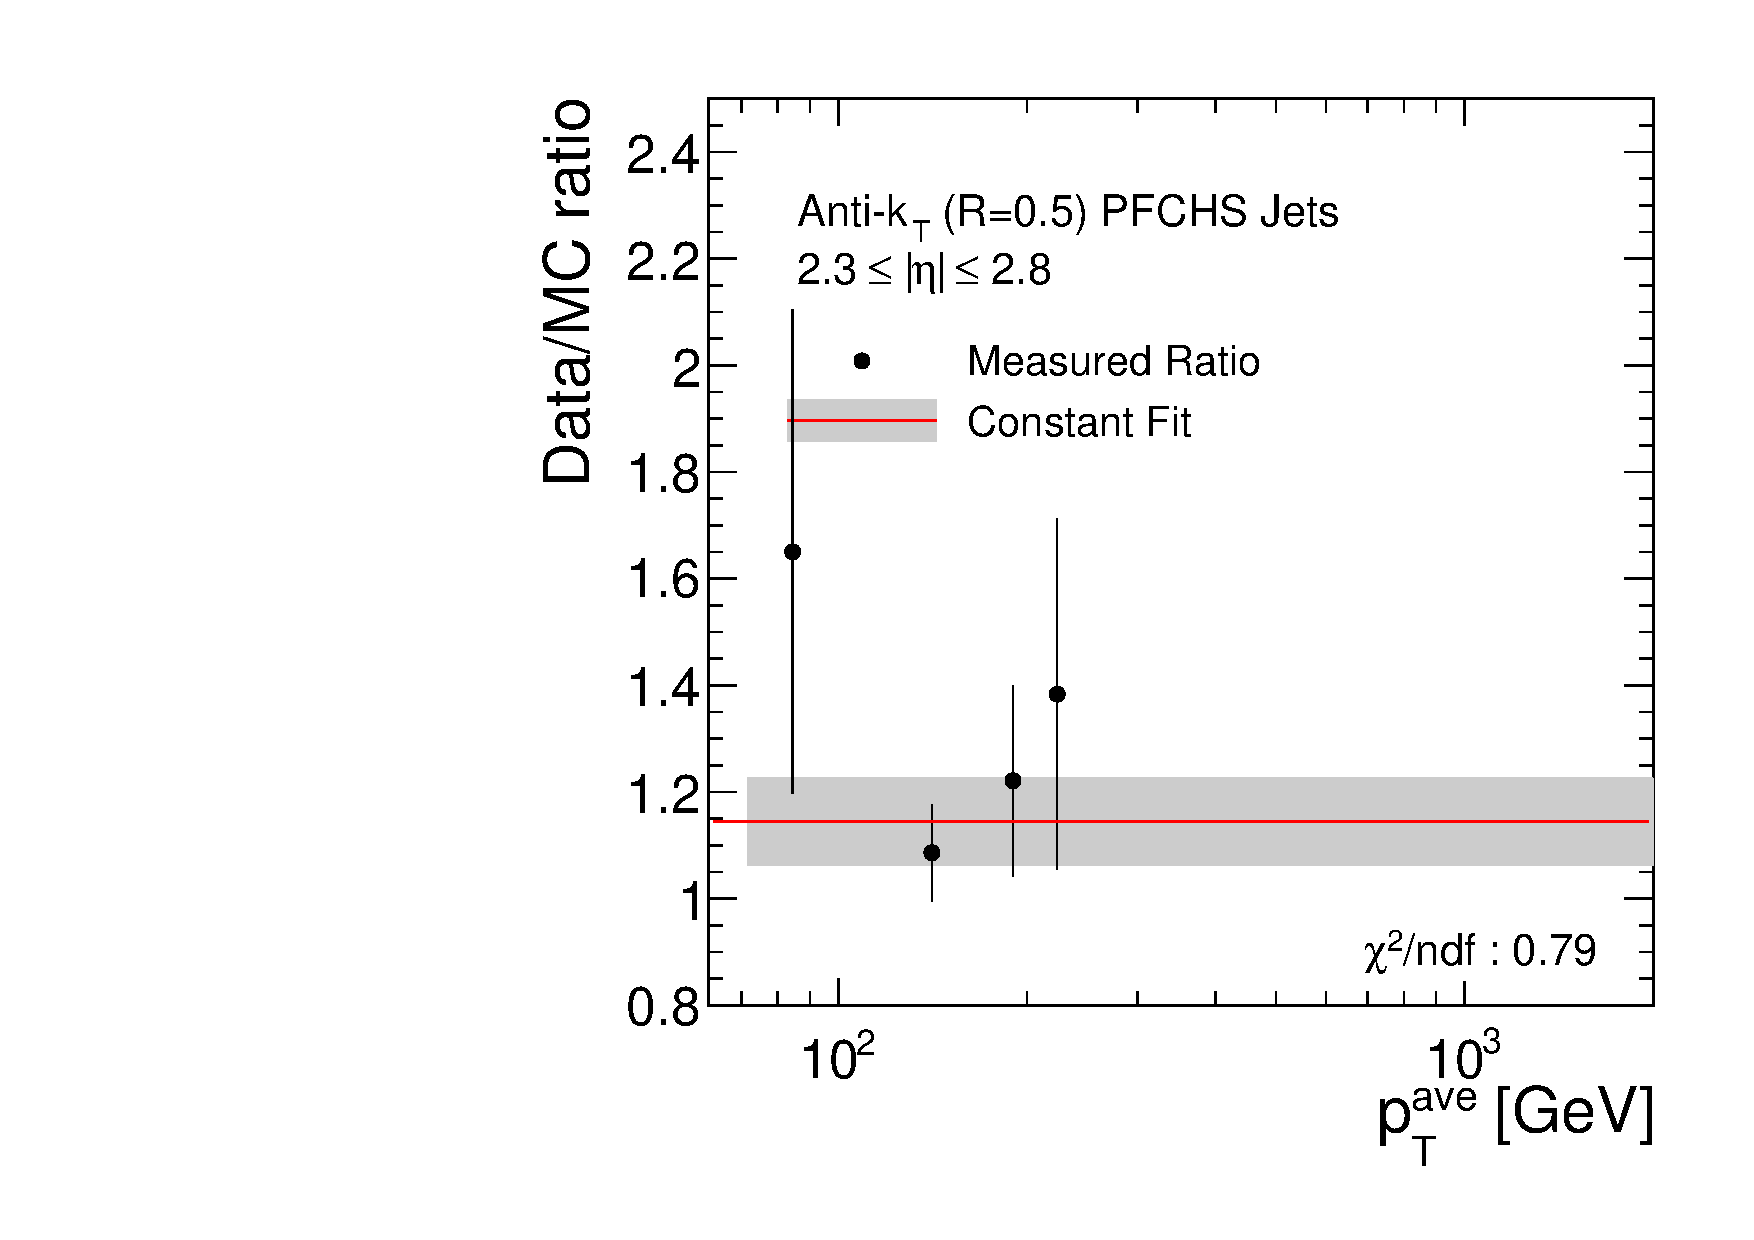
\includegraphics[width=0.49\textwidth]{figures/ExtrapolRatio_Eta4_with_pli_final_nominal_v4b.pdf}
  \end{tabular}
  \caption{Ratio of the resolution in data to the resolution in the \pythia QCD sample in non-empty $|\eta|$ regions as a function of $\pt^\mathrm{ave}$ shown together with a constant fit (red line) and corresponding statistical uncertainty (grey shaded area).}
  \label{fig:ratio}
\end{figure}
After applying all corrections described in Sec.~\ref{sec:jer_corrections}, the measured resolution in data and simulation can be compared by calculating the data-to-simulation ratio

\begin{equation}
  c(\mathrm{Data}/\mathrm{MC}) = \frac{ \sigma_\mathrm{JER,\, Data}}{ \sigma_\mathrm{JER,\, MC}} \, .
 \end{equation}
The resulting distributions as function of $\pt^\mathrm{ave}$ for the different $|\eta|$ regions are shown in Fig.~\ref{fig:ratio}. As no significant \pt-dependence is observed, the ratio is parametrized by a constant fit. In each $|\eta|$ region, the fit result shows a value larger than one. This means that the resolution in data is in general worse than in simulation. The constant fit is also visualized in Fig.~\ref{fig:ratio} (red line) together with the statistical uncertainty resulting from the fit (grey shaded area). The description with a constant seems justified, as the values of $\chi^2/\mathrm{ndf}$, also displayed in Fig.~\ref{fig:ratio}, resulting from the fit are in agreement with one. However, a potential hidden trend as function of \ptave is considered as systematic uncertainty of the measurement. \\
The determined data-to-simulation ratios are summarized later together with statistical and systematic uncertainties in Tab.~\ref{tab:syst_uncert_summary}. Due to statistical limitations, no data-to-simulation ratio could be determined for the two highest $|\eta|$ intervals. As jets in the forward region of the detector have essentially low transverse momentum, these $|\eta|$ intervals are mainly affected by the high pre-scales of the triggers with low momentum thresholds.   
 
\section{Validation of the Method}
\label{sec:jer_validation}
\begin{figure}[!tp]
  \centering
  \begin{tabular}{cc}
                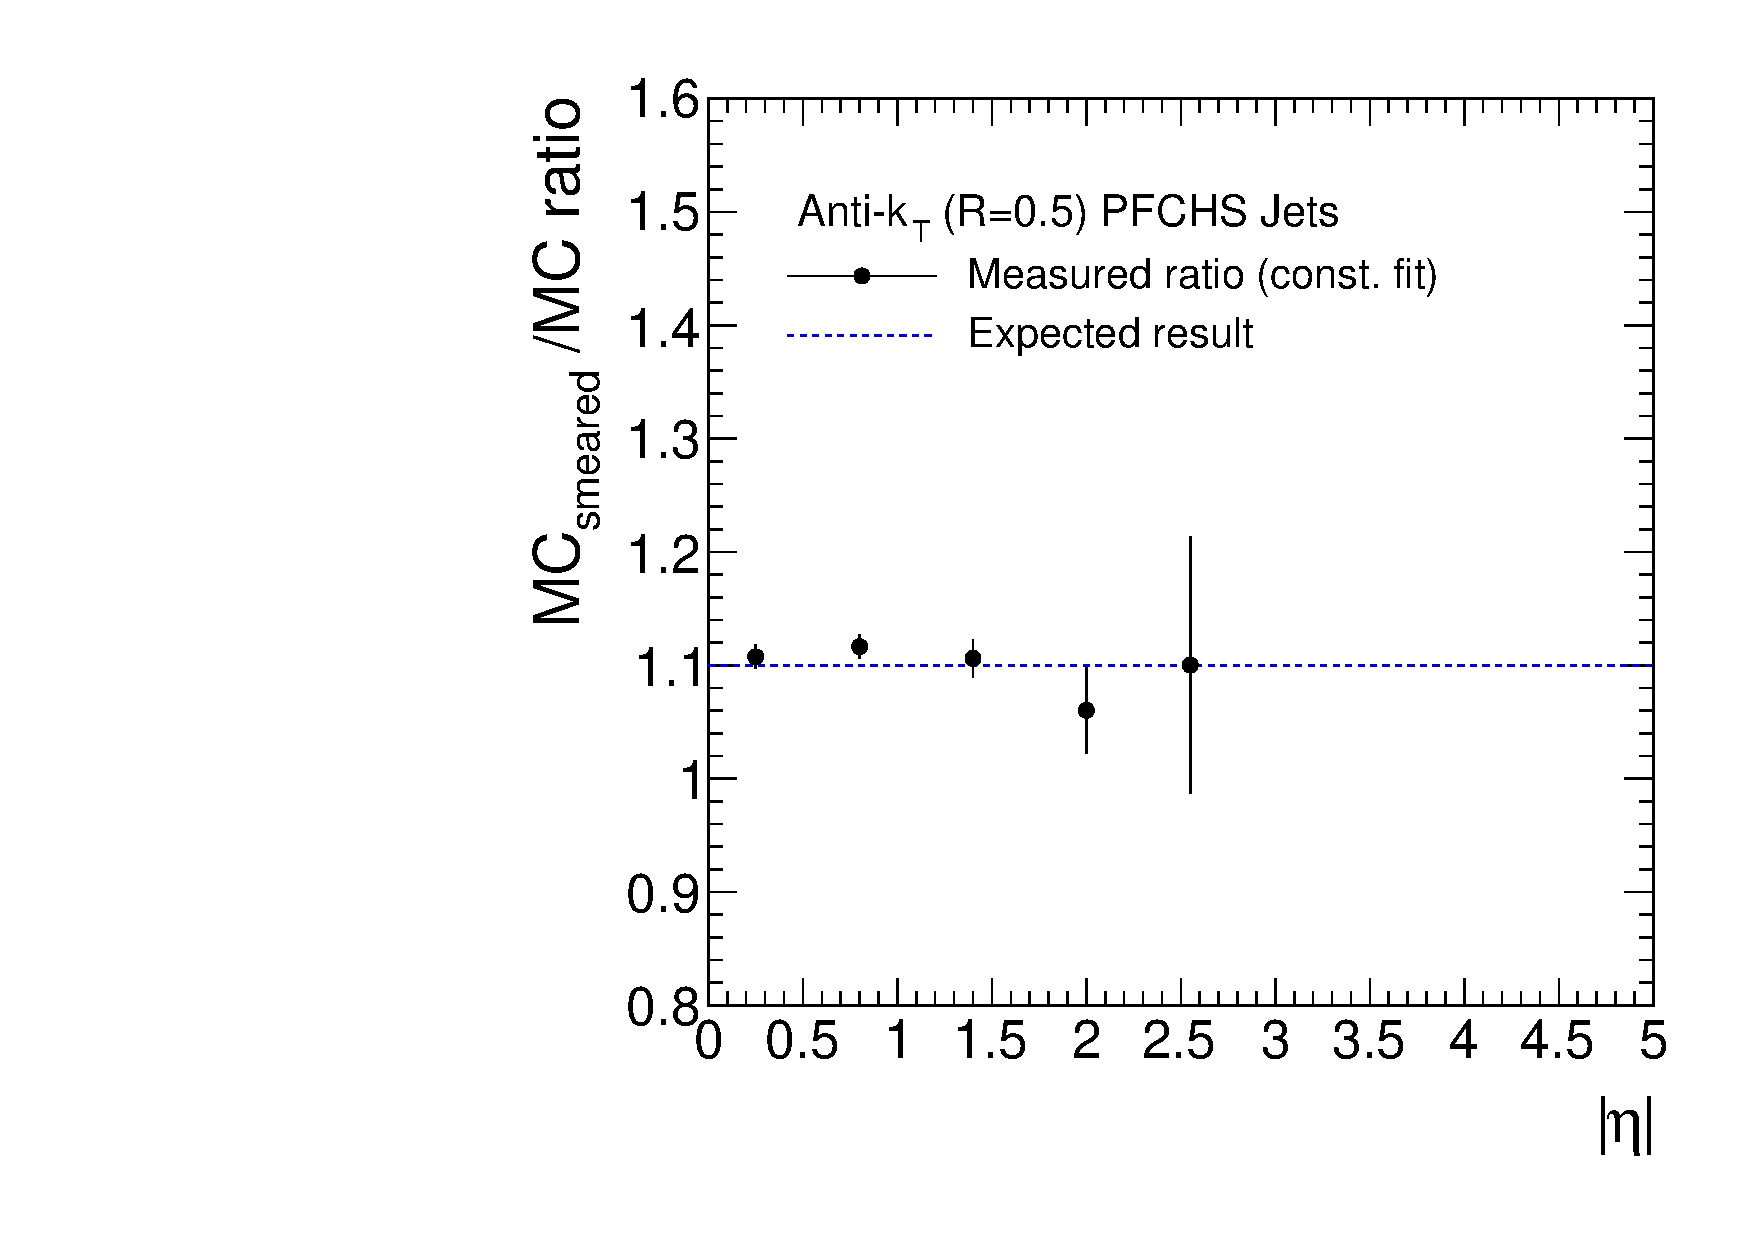
\includegraphics[width=0.49\textwidth]{figures/ScalingFactorsVsEta_with_pli_PythiaSmearedVsPythia_v4b.pdf} &
                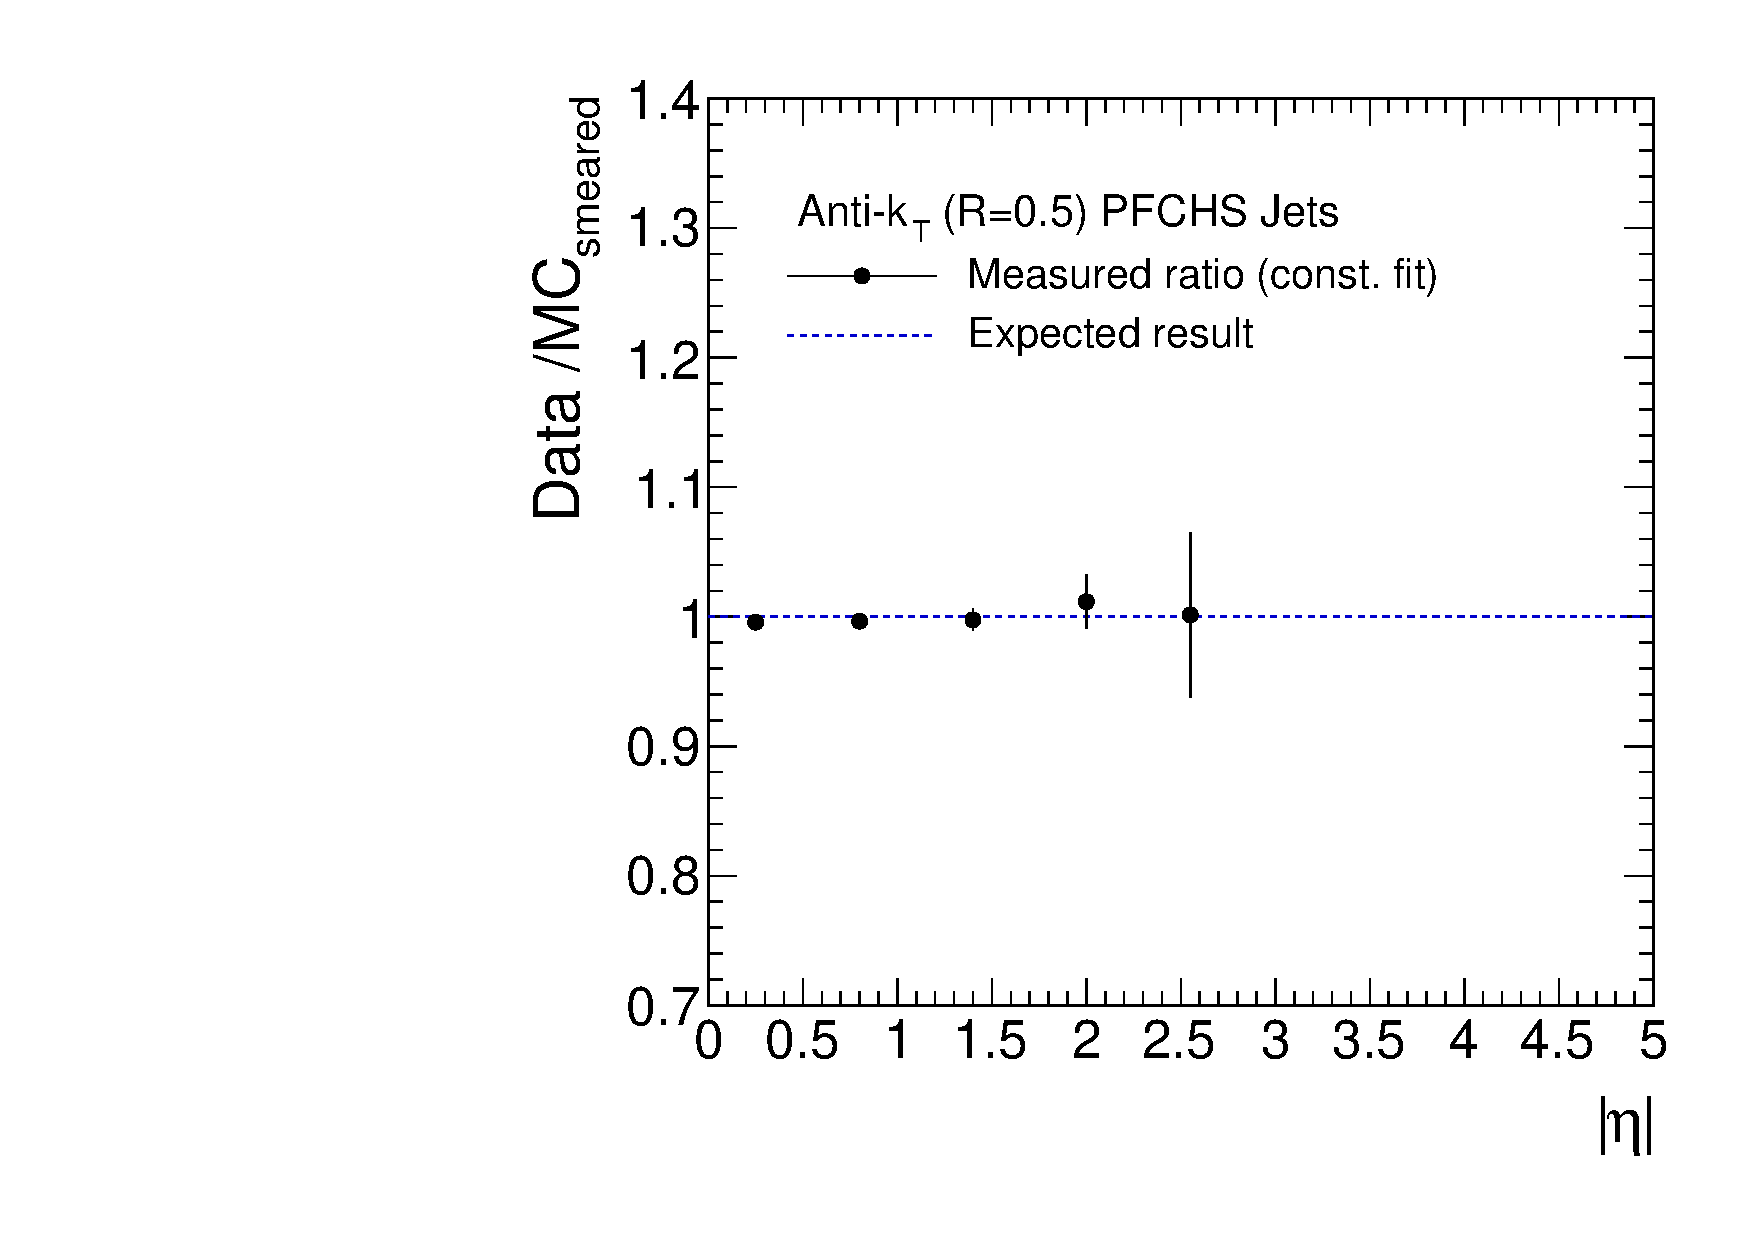
\includegraphics[width=0.49\textwidth]{figures/ScalingFactorsVsEta_with_pli_MCSmearedWithMeasuredValues_final_v4b.pdf}
  \end{tabular}
  \caption{Ratio $c\mathrm{(MC_{smeared}/MC)}$ of the resolution in the smeared QCD sample to the resolution of the unsmeared QCD sample as a function of $|\eta|$ with statistical uncertainty (\textit{left}) and ratio $c\mathrm{(Data/MC_{smeared})}$ of the resolution in data to the resolution of the QCD sample smeared with the measured data-to-simulation ratio as function of $|\eta|$ with statistical uncertainty (\textit{right}). The line indicates the target value of each validation test.}
  \label{fig:mc_closure}
\end{figure}
\subsection{Validation in Simulated Events}
\label{sec:jer_validation_closure}
In order to test the quality of the method to predict the correct data-to-simulation ratio, a validation test based on simulated events is performed. \\ 
In this test, the simulated \pythia QCD sample is divided into two sub-samples with equal number of events. In one of the sub-samples the leading corrected jets\footnote{It is necessary to correct all jets which might get relevant for the analysis, \ie become one of the three leading jets. In this analysis the five leading jets in \pt are corrected.} in \pt in each event are smeared with a smearing factor $c$ which increases the \pt resolution. This is done for jets which pass a minimum \pt threshold of 10\gev. More precisely this means that for each reconstructed jet that has a corresponding generated jet within a $\Delta R < 0.25$ cone, the transverse momentum is scaled according to
\begin{equation}
 p_\mathrm{T}' = p^\mathrm{gen}_\mathrm{T} + c \cdot (p_\mathrm{T} - p^\mathrm{gen}_\mathrm{T}) \, .
\label{eq:smear_gen}
\end{equation} 
resulting in the smeared momentum $\pt'$. After the smearing procedure, the jet momenta are re-ordered descendent in \pt.\\
For this test, the smearing factor has been chosen to be $c = 1.1$ for each $|\eta|$ interval. This is expected to be the resulting ratio when determining the ratio of the resolution in the smeared QCD sub-sample to the resolution in the unsmeared sub-sample derived with the asymmetry method including all corrections as described in Sec.~\ref{sec:jer_corrections}. Consequently, the test is passed when the measured ratio recovers the input value according to $c\mathrm{(MC_{smeared}/MC)} = 1.1$. The resulting values obtained from a constant fit of the ratios as a function of $\pt^\mathrm{ave}$ are shown in each $|\eta|$ region with statistical uncertainties in Fig.~\ref{fig:mc_closure} (left). It can be seen that the input scaling factor of 1.1 is well recovered with this procedure within the statistical uncertainties. Thus, a potential resolution difference when comparing data and simulation can be determined with this approach as well.

\subsection{Validation of the Measured Data-to-Simulation Ratio}
\label{sec:jer_validation_ratio}
In addition to the validation test on simulated events, also the measured data-to-simulation ratio can be directly validated. This is done with a similar approach as described in Section~\ref{sec:jer_validation_closure}.\\
For the test of the measured data-to-simulation ratio, the individual jet momenta in the simulated \pythia QCD sample are scaled with the measured resolution ratio values $c{(\mathrm{Data}/\mathrm{MC})}$ according to Eq.~\ref{eq:smear_gen}. Thus, jets are corrected with different scale factors depending on the respective $|\eta|$ region they belong to. After applying the smearing procedure to the jet momenta in simulation, the whole measurement procedure of the data-to-simulation including the corrections for further jet activity and PLI is performed. Since the measured resolution differences between data and simulation have been compensated before the actual re-determination of the data-to-simulation ratio, it is expected to obtain ratios of $c\mathrm{(Data/MC_{smeared})} = 1$. The result of this test is illustrated in Fig.~\ref{fig:mc_closure} (right) with statistical uncertainties. A good agreement with the expected value of 1 is visible, even without the consideration of systematic uncertainties in this consistency test. This again proves that the dijet asymmetry method is well suited to determine resolution differences between data and simulation, expressed in the data-to-simulation ratio. 

\section{Systematic Uncertainties}
\label{sec:jer_syst_unc}
In addition to the uncertainty of the resolution measurement due to statictical effects, there are also systematic components which influence the outcome of the data-to-simulation ratio. The different contributions of systematic uncertainties to the measurement are discussed in this section.\\
All systematic uncertainties are determined by evaluating the shift of the data-to-simulation ratio when varying a certain aspect in the measurement procedure. The uncertainty $\delta c$ is calculated by the determination of the ratio for a certain shift $\Delta$ and comparing it to the nominal ratio 
 \begin{equation}
  \delta c{\mathrm{(Data/MC)}} = c{\mathrm{(Data/MC)}_{\Delta}} - c\mathrm{(Data/MC)}
 \end{equation} 
Thus, all systematic uncertainties are determined as absolute shift of the nominal ratio. Typically, an upward and downward shift is evaluated. Resulting uncertainties are afterwards symmetrized by taking the average shift. If, however, the up- and downward variation both result in either an upward or downward shift, the absolute shift is determined and the maximum of both is taken and quoted as symmetric uncertainty. In case only an up- or downward variation is performed, the systematic uncertainty is taken symmetrically as the absolute shift.   

\begin{description}
 \item[PU reweighting:] The trigger dependent pileup distributions in data, which are used to reweight the simulated sample to match the observed pileup distribution in data, are calculated with a nominal minimum bias cross section of $69.4\,\rm{mb}$. In order to propagate the uncertainty on the minimum bias cross section to the data-to-simulation ratio, it is increased to $73.5\,\rm{mb}$. Hence, the pileup scenario of the simulated \pythia QCD sample is reweighted to the data distributions obtained with this varied minimum bias cross section. Apart from that variation, the measurement of the data-to-simulation ratio is performed as for the nominal ratio. \\
\begin{figure}[!tp]
  \centering
  \begin{tabular}{cc}
                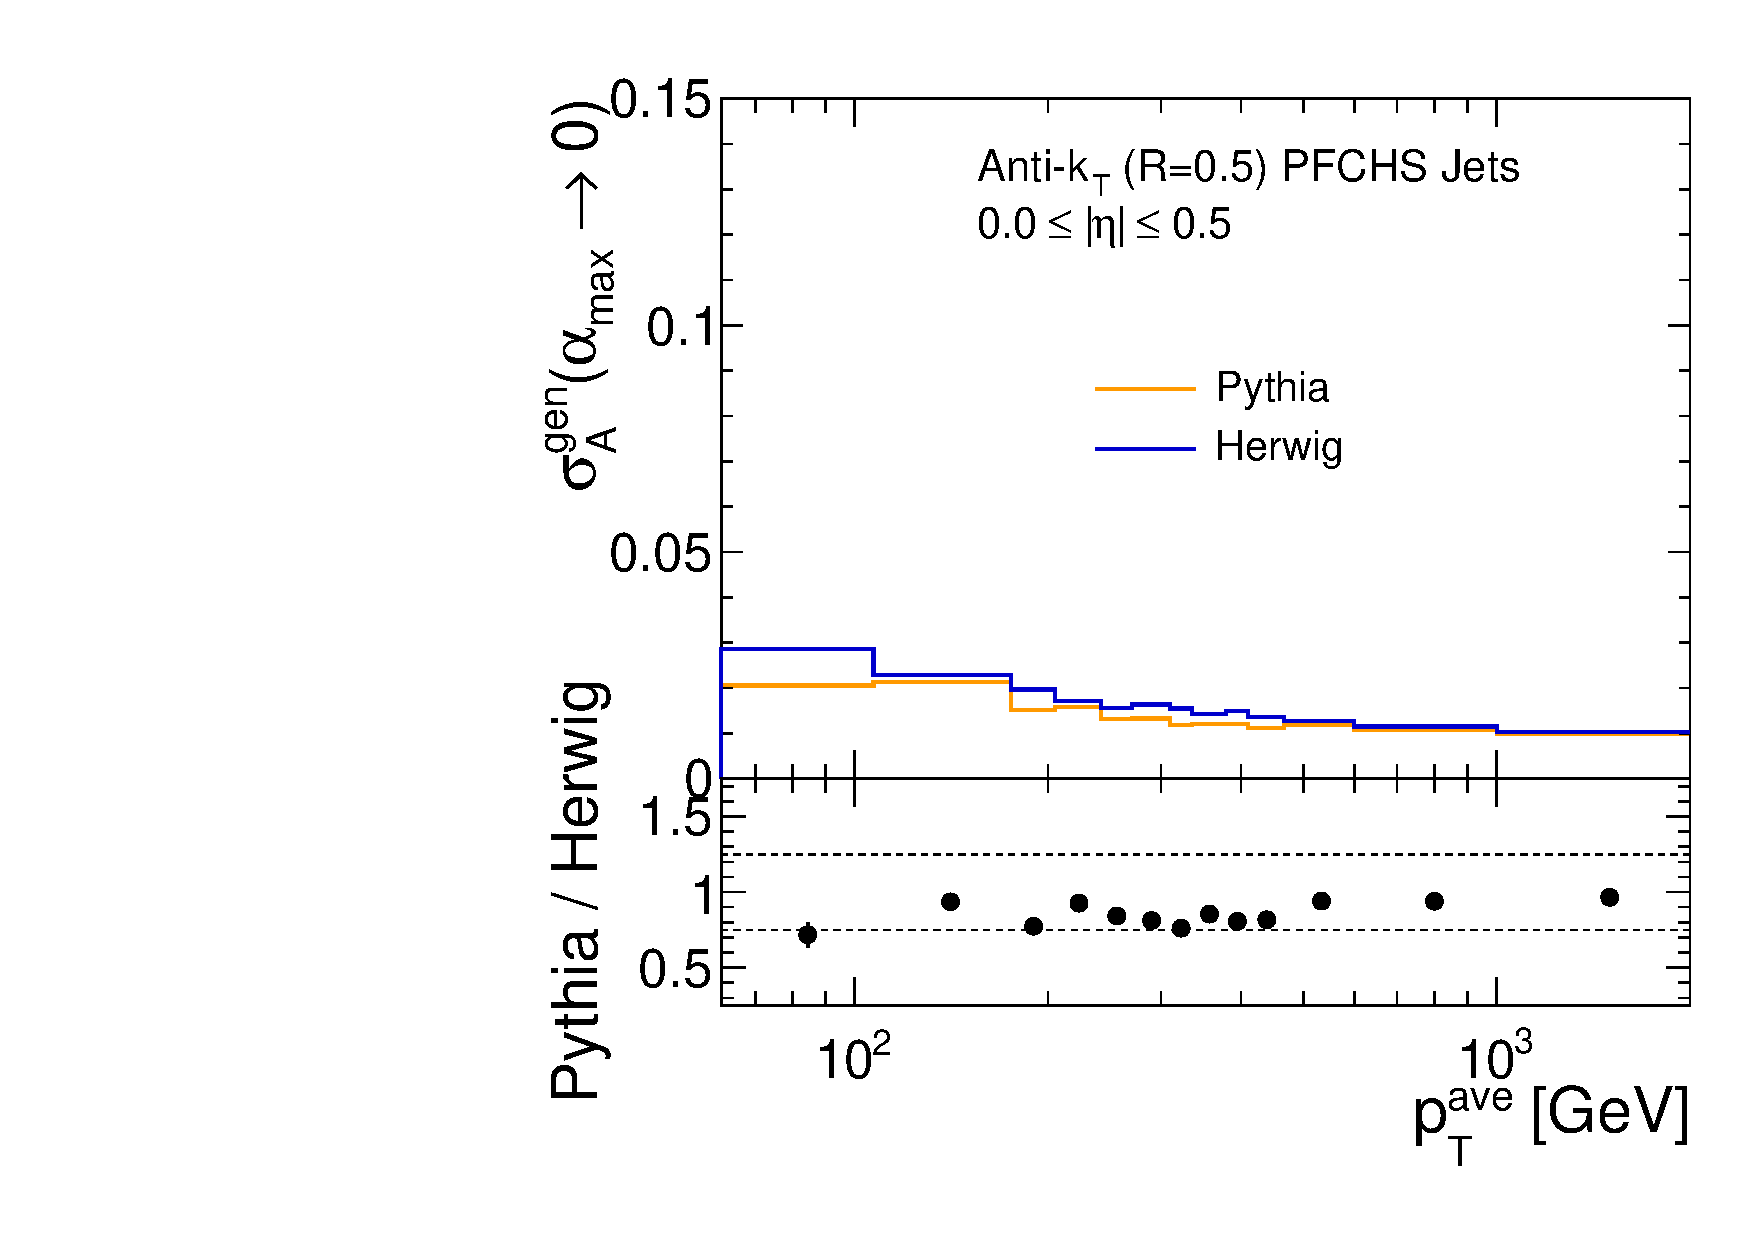
\includegraphics[width=0.49\textwidth]{figures/PLI_comparison_Eta0_v4.pdf} &
                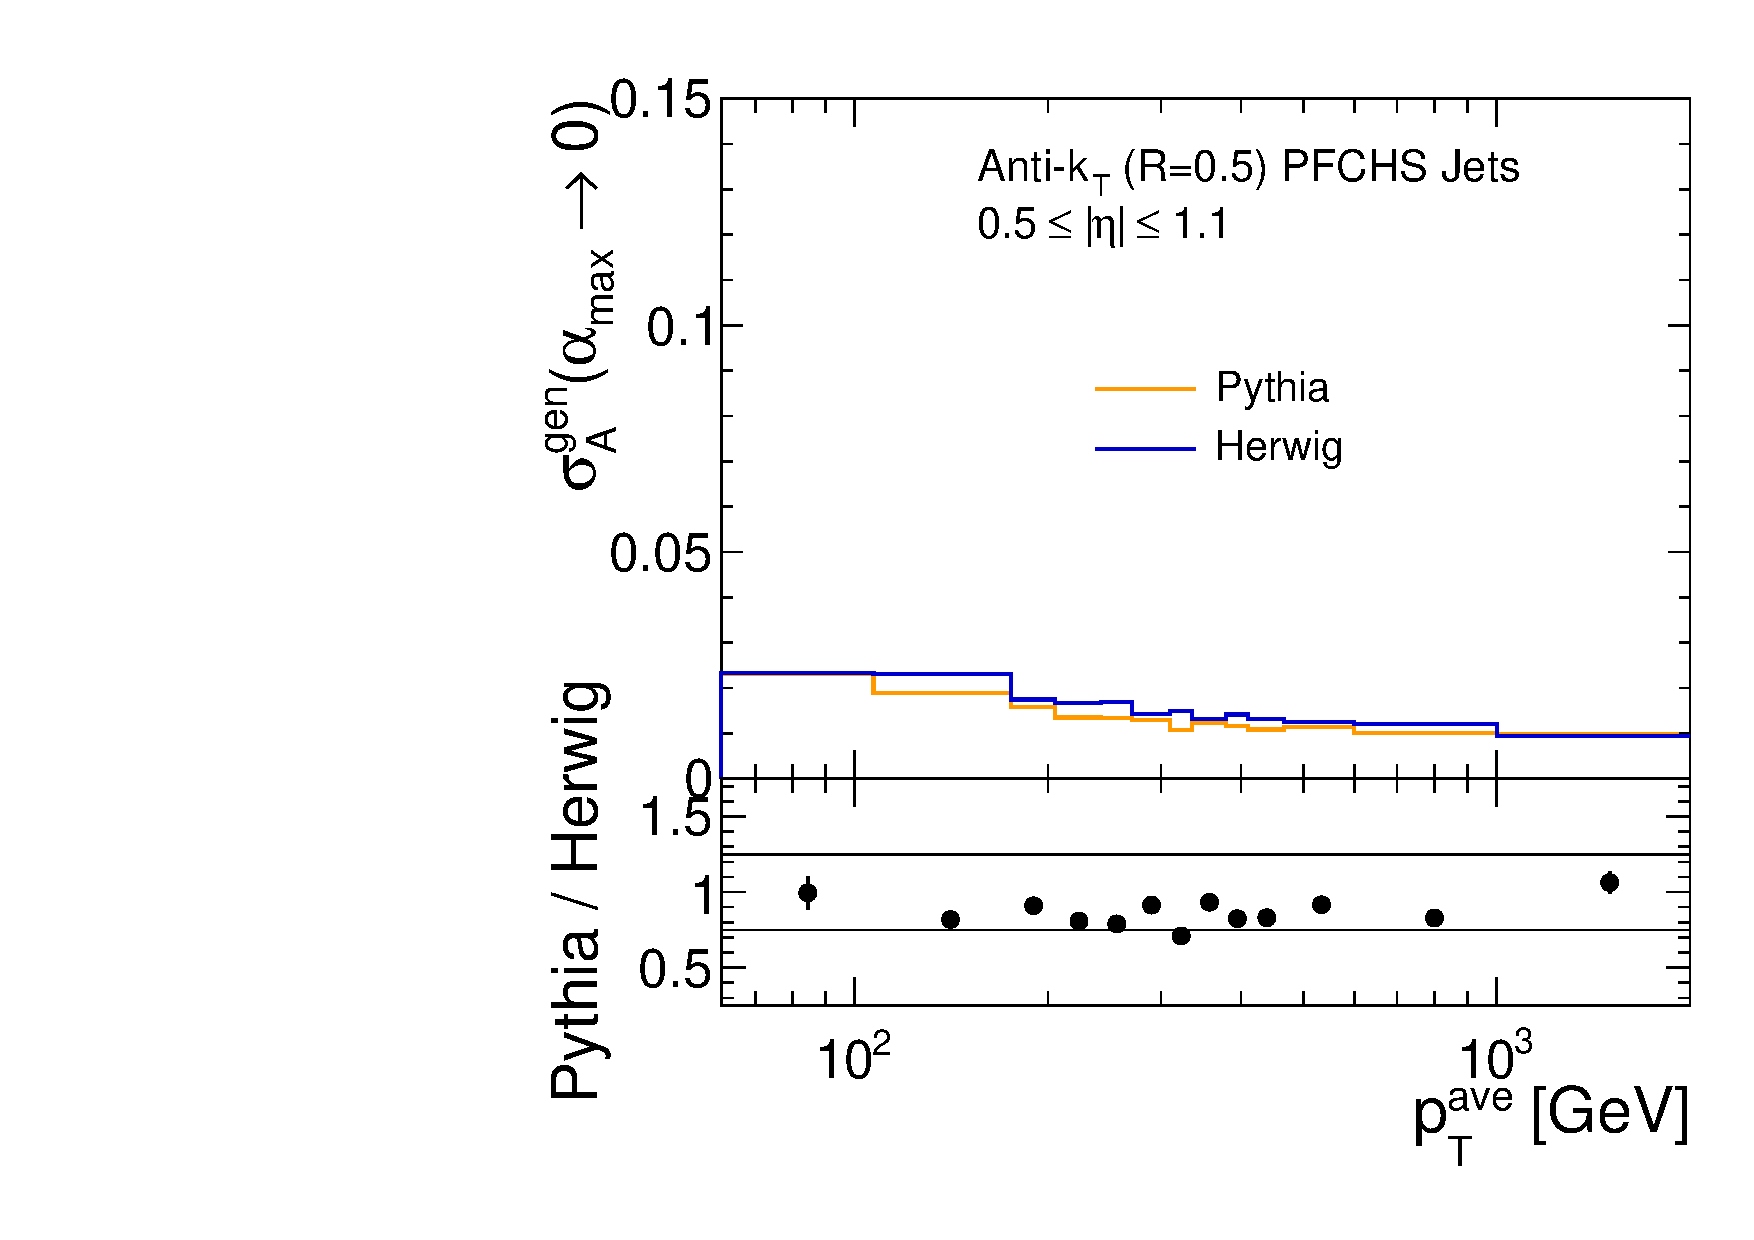
\includegraphics[width=0.49\textwidth]{figures/PLI_comparison_Eta1_v4.pdf} \\
  \end{tabular}
  \caption{Comparison of the contributions to the asymmetry width due to particle-level imbalance in QCD multijet events generated with \pythia (yellow) to the same quantity derived with the \herwig generator (blue) in the two central $|\eta|$ regions as a function of $\pt^\mathrm{ave}$.}
  \label{fig:pli_comp}
\end{figure}
 
 \item[Particle-level imbalance:] 
The measured resolution in data and simulation is corrected for an imbalance at particle level due to out-of-cone showering effects based on simulation. In order to account for the uncertainty on $\sigma_\mathrm{PLI}$, the PLI-correction factor for each measured resolution value is shifted by $\pm 25\%$. Consequently, the changed ratio is calculated as
 \begin{equation}
  c\mathrm{(Data/MC)_{PLI}} = \frac{\sqrt{2} \cdot \sigma^\mathrm{Data}_\mathrm{A}(\alpha_\mathrm{max} \rightarrow 0) \ominus f \cdot \sigma_\mathrm{PLI}}{\sqrt{2} \cdot \sigma^\mathrm{MC}_\mathrm{A}(\alpha_\mathrm{max} \rightarrow 0) \ominus f \cdot \sigma_\mathrm{PLI}}  
 \end{equation}
with $f=0.75, 1.25$ respectively. The size of this variation is chosen by comparing the size of the PLI correction in simulated events from the nominal \pythia sample to the PLI correction estimated from simulated events obtained by the \herwig generator with tune EE3C. This comparison is illustrated in Fig.~\ref{fig:pli_comp} for the two central $|\eta|$ regions. Since the size of the PLI correction agrees within $25\%$ between both generators, the size of this uncertainty is justified.
 
 \item[Jet energy scale:] The jet energy scale has been corrected to particle level by the application of dedicated calibration factors. In order to propagate the uncertainty of the jet energy scale corrections to the data-to-simulation ratio of the resolution, all jet momenta in the simulated sample are shifted up and down by the JEC uncertainty. The jet momenta in data stay unchanged. Afterwards, the data-to-simulation is determined again based on the varied jet momenta.

 \begin{figure}[!tp]
  \centering
  \begin{tabular}{cc}
                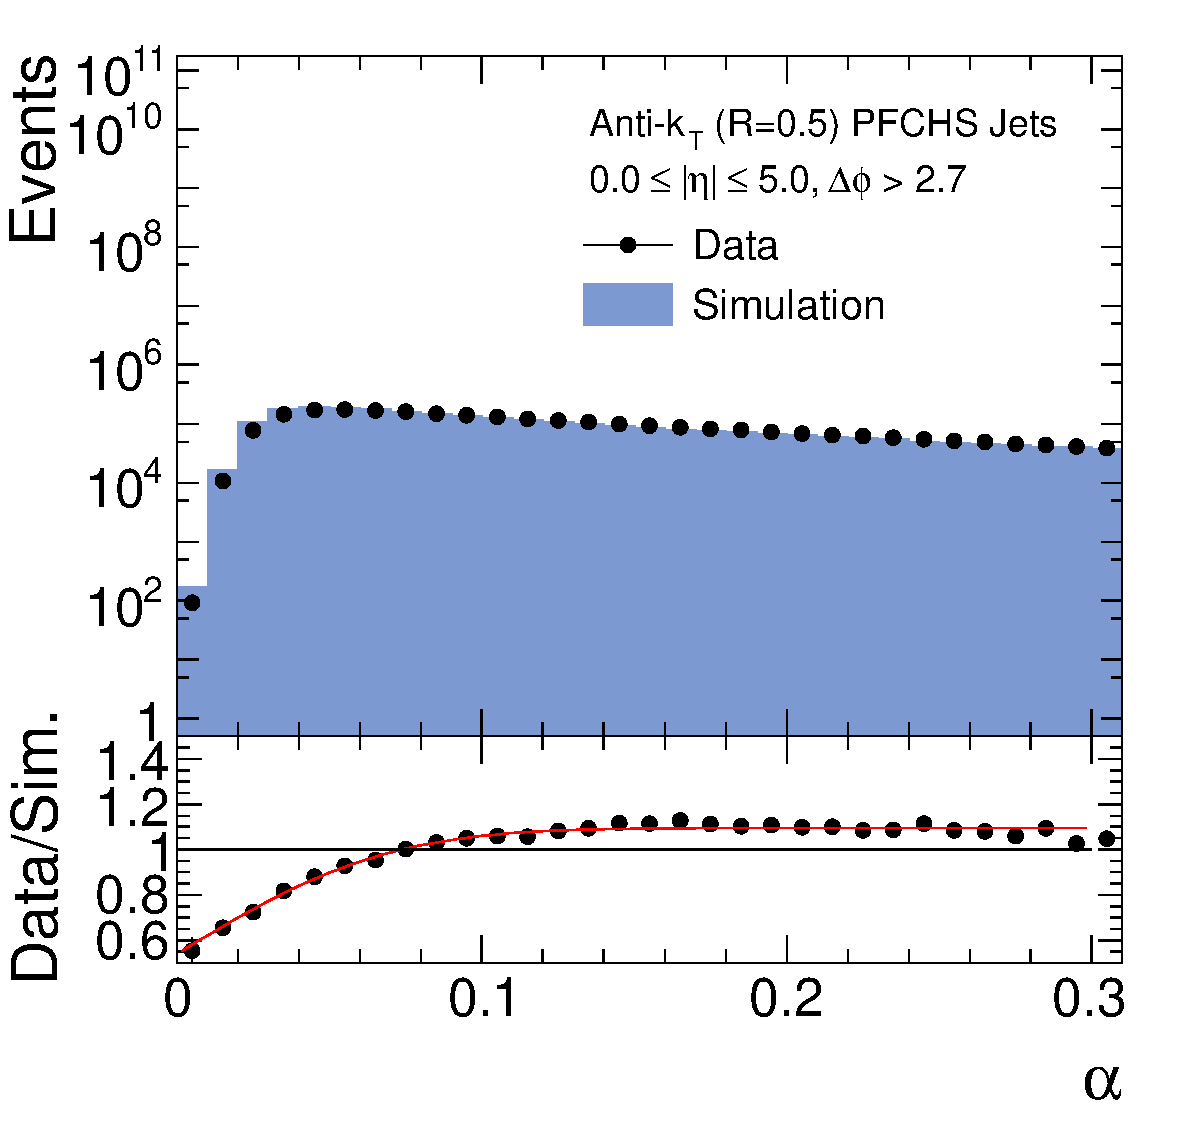
\includegraphics[width=0.49\textwidth]{figures/Alpha__AfterAsymmHistos.pdf} &
                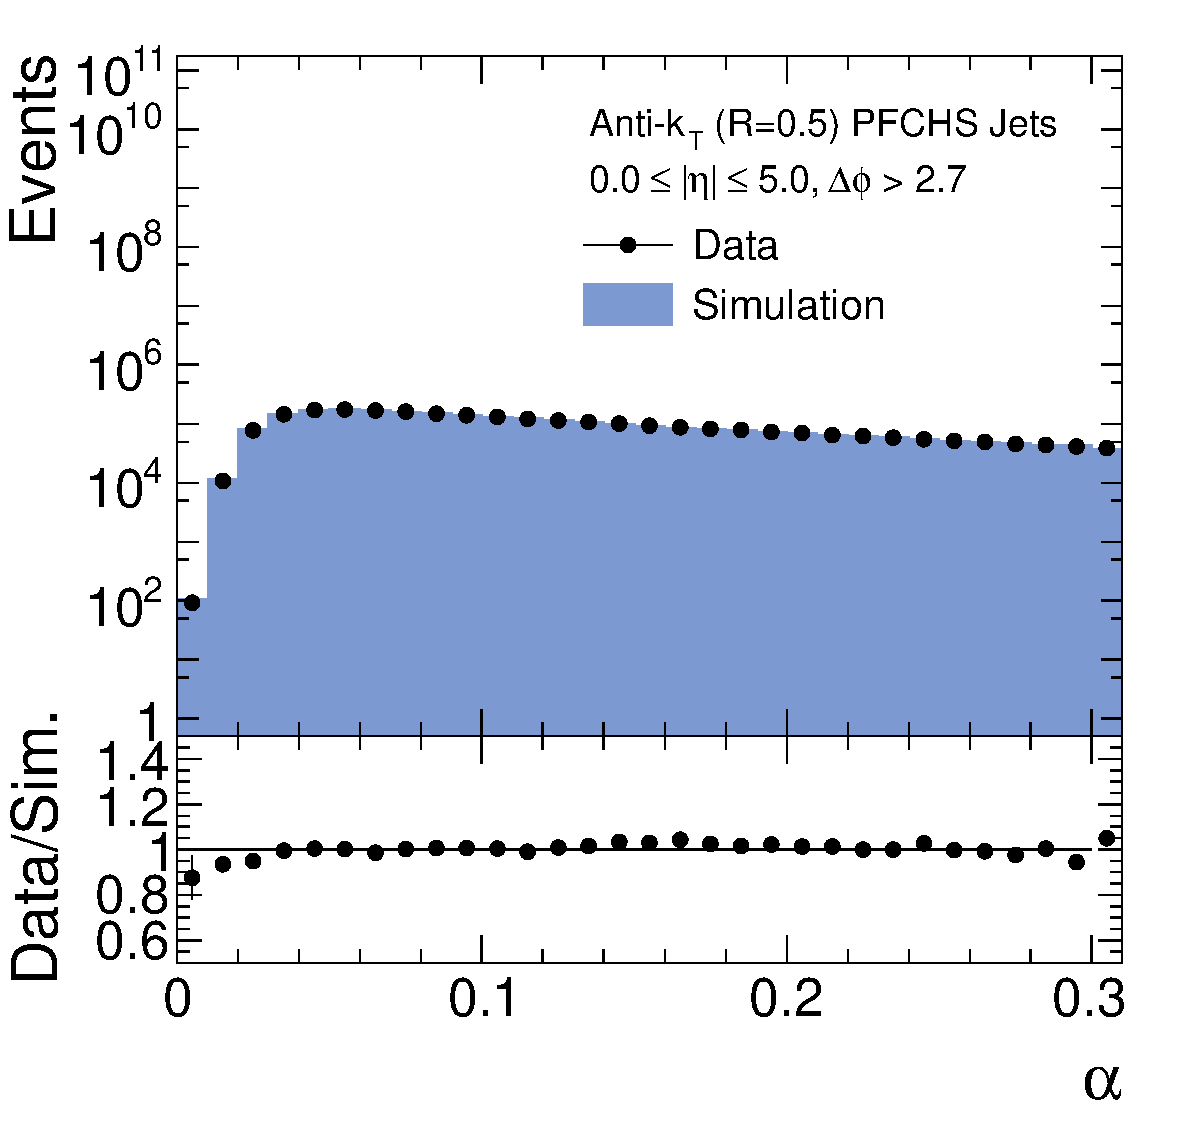
\includegraphics[width=0.49\textwidth]{figures/AfterReweight_Alpha__AfterAsymmHistos.pdf}
  \end{tabular}
  \caption{Inclusive $\alpha$-spectrum before (\textit{left}) and after (\textit{right}) reweighting the $\alpha$-spectrum of the simulated sample. The red curve in the bottom of the left plot illustrates the function used for the $\alpha$-spectrum reweighting.}
  \label{fig:syst_uncert_alpha_spec}
\end{figure}
 
 \item[$\alpha$-spectrum:] To account for additional jet activity in the event, the measured widths of the asymmetry distributions are extrapolated to zero additional jet activity by a linear function. This linear behaviour is an empirically found relation rather than a theoretically fundamental connection. One influencing factor of the linear behaviour is the functional form of the $\alpha$-spectrum. It determines how many events are added to the asymmetry distribution in the next higher $\alpha$ interval and consequently how much the asymmetry distribution is broadened. This can result, \eg in a smaller or larger slope of the linear function or result in a non-linear behaviour. However, such effects might cancel in the ratio as long as the $\alpha$-spectrum is the same in data and simulation. \\
 The observed inclusive $\alpha$-spectrum in the simulated sample is compared to the spectrum in data and shown in Fig.~\ref{fig:syst_uncert_alpha_spec} (left). The bottom part displays the ratio $\rm{Data/MC}$. Since the ratio shows that both spectra do not agree, the influence of the $\alpha$-spectrum on the data-to-simulation ratio is evaluated by reweighting the $\alpha$-spectrum in simulated events to roughly match the one observed in data. The red curve overlaid in the ratio of the left distribution is used to reweight the events in the simulation. For each event a weight $w(\alpha)$ is calculated according to 
\begin{equation}
w(\alpha) = 0.545 \cdot \mathrm{(erf}(13.5 \cdot \alpha -0.02) +1))
\end{equation}
with the error function erf\footnote{ $\mathrm{erf(x)} = \frac{1}{\sqrt{\pi}} \int\limits_{-x}^{x} e^{-t^2} dt$}. This weight is considered as multiplicative factor onto the usual event weight in simulation. For comparison, the reweighted $\alpha$-spectrum is shown in the right part of Fig.~\ref{fig:syst_uncert_alpha_spec}.
 
 \item[$\alpha$-range:] In addition to the functional form of the $\alpha$-spectrum, also the specific range which has been chosen for $\alpha$ can result in a more or less linear behaviour of the measured asymmetry widths. The choice of the linear function implies that the linear behaviour holds also for small values of $\alpha$. However, especially for small values of $\alpha$ the linear behaviour could not be tested explicitly due to the imposed minimum \pt threshold of 10\gev for the third jet. \\
In order to study the linear behaviour of the extrapolation also towards smaller $\alpha$-values, the minimum \pt cut of 10\gev for the third jet is dropped and an additional $\alpha$-interval 0.0--0.05 is introduced for the measured asymmetries at detector level as well as the PLI correction. In Fig.~\ref{fig:syst_uncert_alpha_range}, some example extrapolations of the asymmetry widths in data and simulation with the additional $\alpha$-interval are shown. The resulting difference to the nominal data-to-simulation ratio is considered as systematic uncertainty.

\begin{figure}[!tp]
  \centering
  \begin{tabular}{cc}
                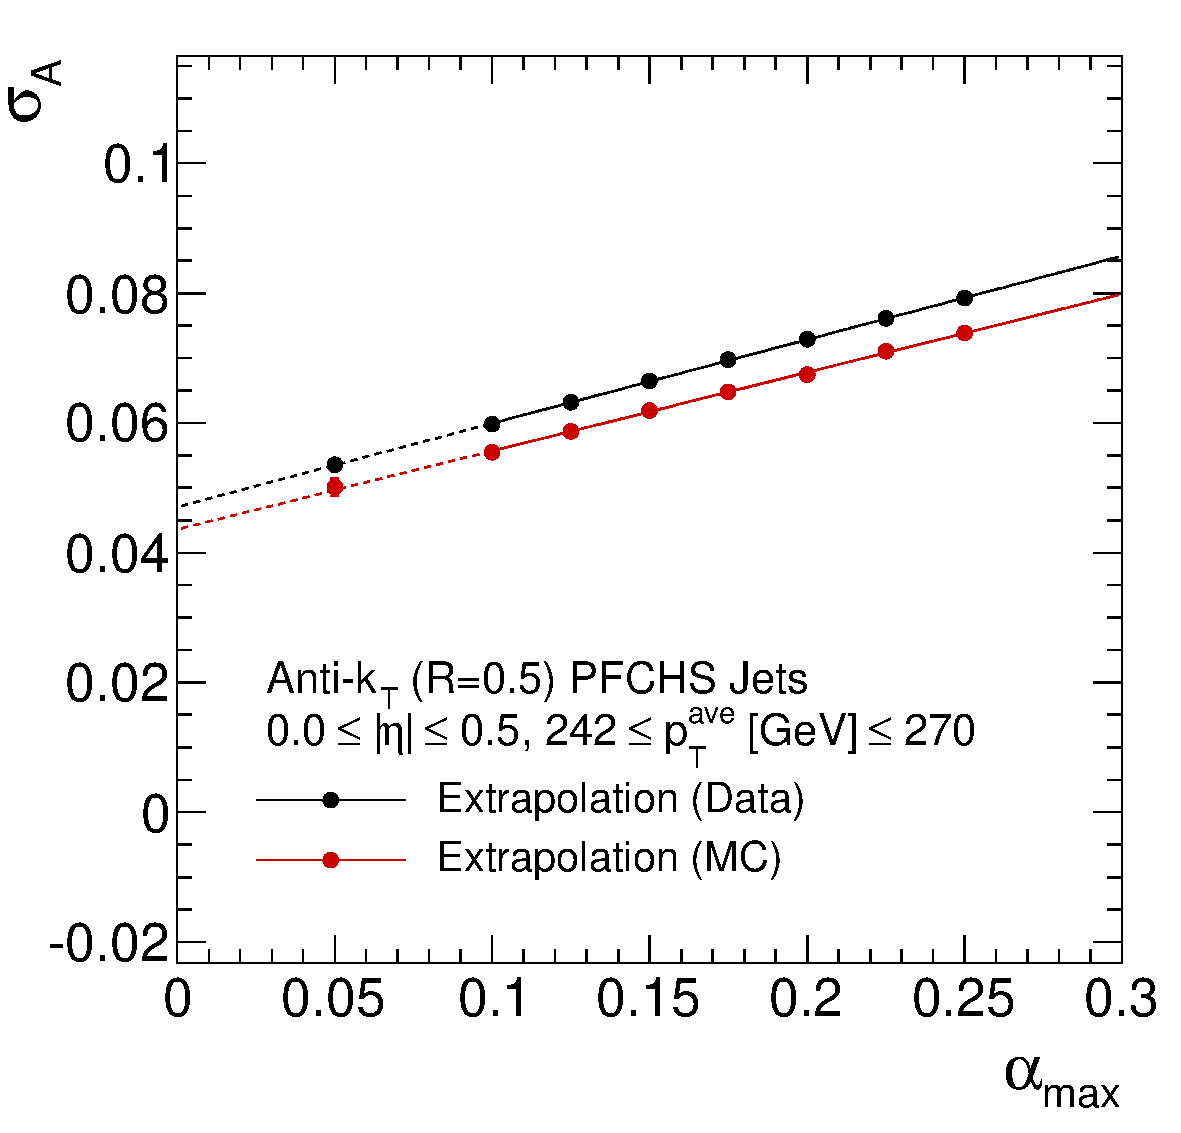
\includegraphics[width=0.49\textwidth]{figures/Extrapol_Eta0_pt4_final_nominal_NoMinPtCutForThirdJet_AddNewAlphaBin_v4.pdf} &
                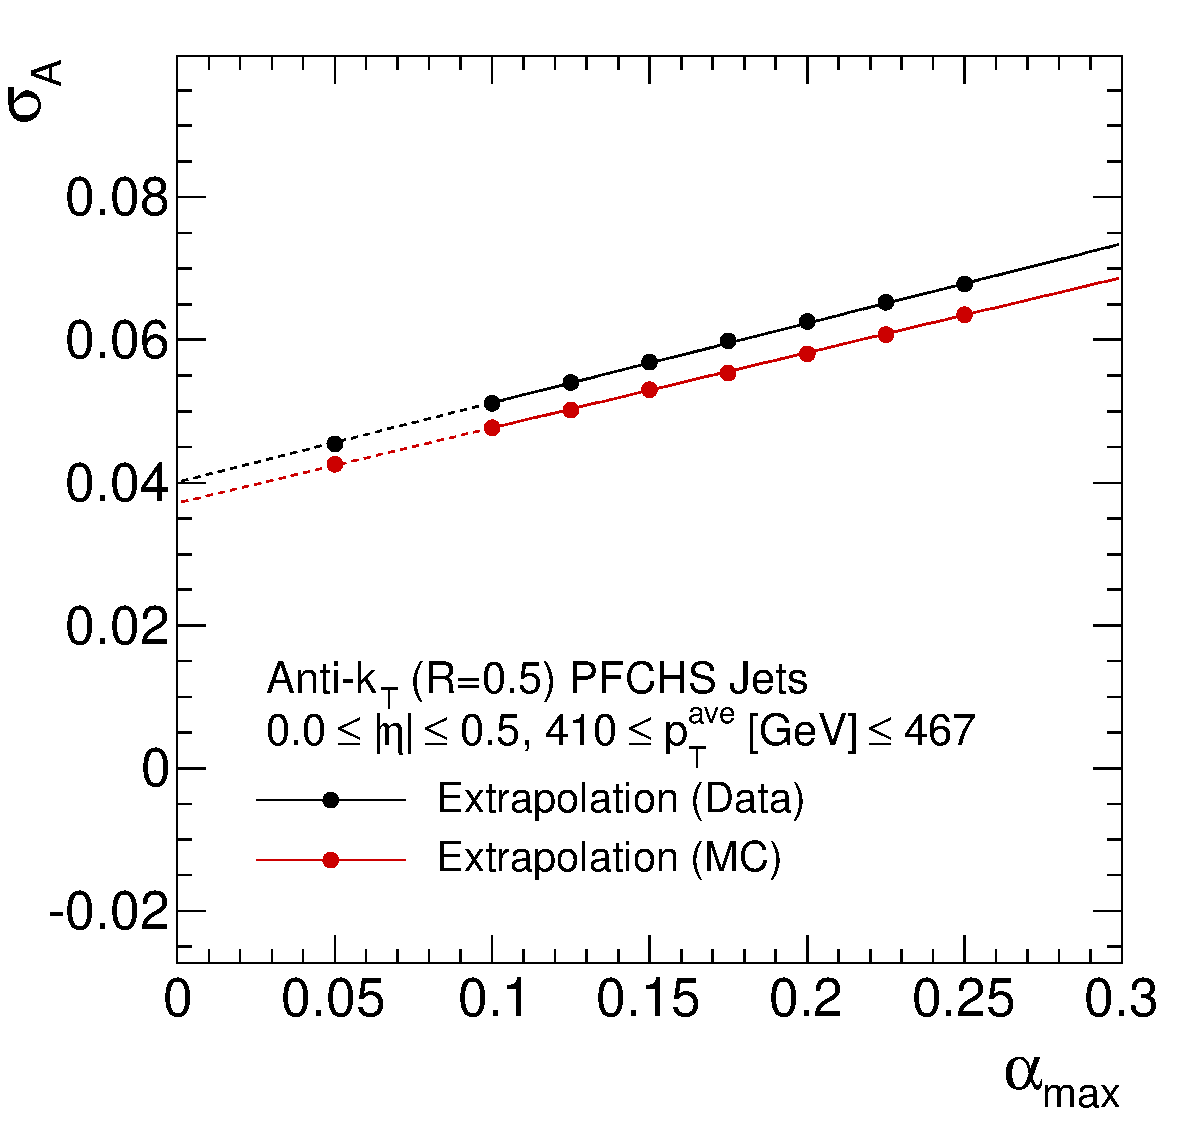
\includegraphics[width=0.49\textwidth]{figures/Extrapol_Eta0_pt9_final_nominal_NoMinPtCutForThirdJet_AddNewAlphaBin_v4.pdf}
  \end{tabular}
  \caption{Two example extrapolations of measured values for $\sigma_\mathrm{A}$ in data and simulation to obtain the result at zero additional jet activity when adding one additional $\alpha$ interval 0.0--0.05.}
  \label{fig:syst_uncert_alpha_range}
\end{figure}

\item[Non-Gaussian tails:] As discussed in Sec.~\ref{sec:jer_asymm_width_def}, the width of the asymmetry distribution is calculated as a truncated root-mean-square in order to reject contributions from non-Gaussian tails. The truncation was chosen to be 1.5\% for both data and simulation. In general, it is possible that the tail contributions in data and simulation differ and consequently do not cancel out in the ratio. In order to evaluate this effect the data-to-simulation ratio is calculated when truncating 5\% of the original distribution instead of 1.5\%.  

\item[Flavour uncertainty:] As discussed in Sec.~\ref{sec:jer_response}, the jet response can be quite different for light-flavour ($u,d,s$) and heavy-flavour quarks ($c,b$). If the flavour composition is the same in data and simulation, this flavour difference cancels out in the data-to-simulation ratio. Since it is known that especially the rate of gluon splitting events with $g \rightarrow b\bar{b}$ is modelled wrong by about a factor of two~\cite{Khachatryan:2011wq}, the impact of heavy quarks produced in gluon splitting processes on the data-to-simulation ratio is evaluated by varying the event weights for simulated events with gluon splitting into heavy-flavour quarks.\\
An event is considered as gluon splitting event, if one of the two leading jets undergoes a gluon splitting identified by utilizing generator truth information. All events identified as gluon splitting into heavy-flavour quarks get an event weight of 1.5. Afterwards, the data-to-simulation ratio is derived as the resolution from data to the resolution in the reweighted simulated sample. 
%An event is considered as gluon splitting event, if one of the two leading jets has a gluon jet flavour with respect to the physics definition for jet flavour. It is distinguished between gluon splitting into light and heavy jets by identifying if the jet considered as gluon in the physics definition has a b/c-flavour or a light flavour using the algorithmic definition. All events where at least one of the two leading jets is identified as a gluon splitting into heavy quarks get an event weight of 1.5. Afterwards the data-to-simulation ratio is derived as the resolution from data to the resolution in the reweighted simulated sample.

\begin{figure}[!p]
  \centering
  \begin{tabular}{cc}
                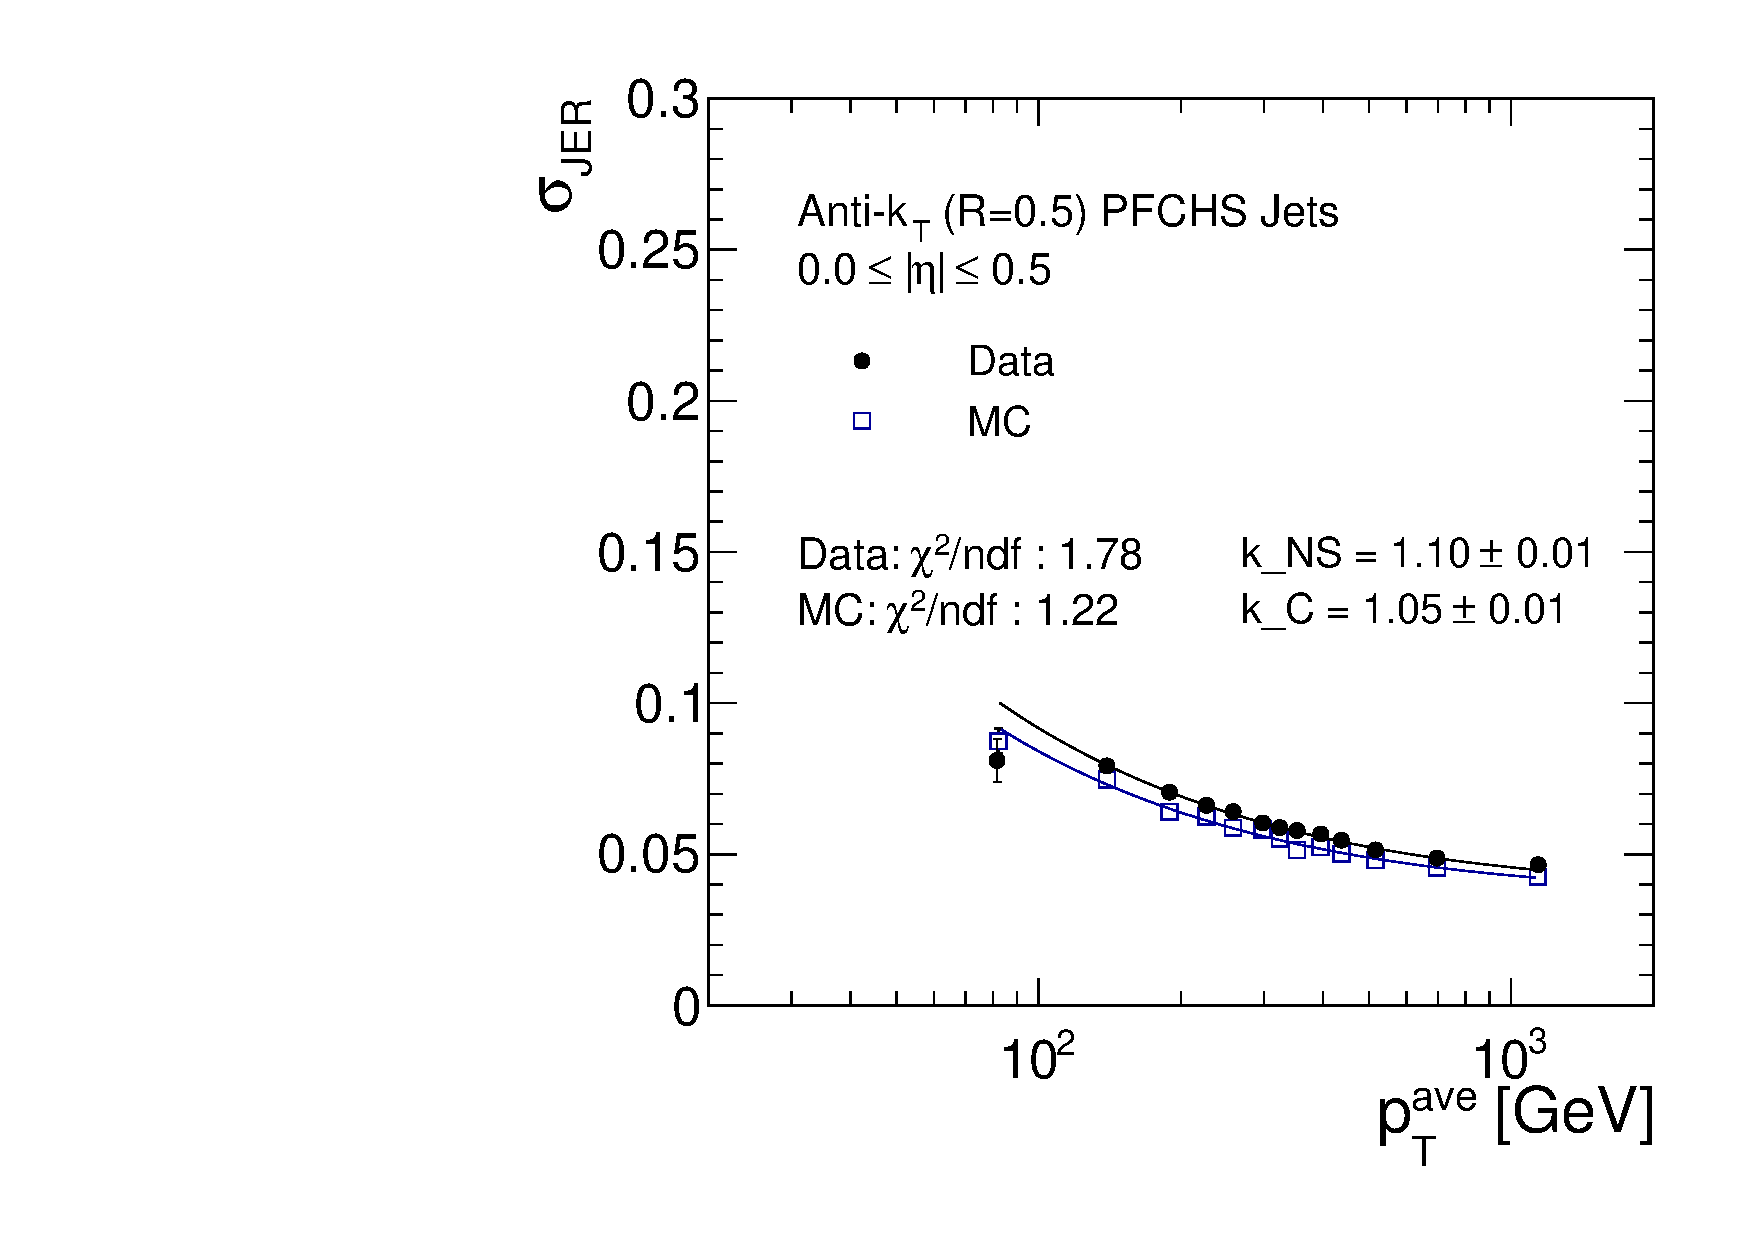
\includegraphics[width=0.49\textwidth]{figures/Pythia_NSCFit_Eta0_kNS_kC.pdf} &
                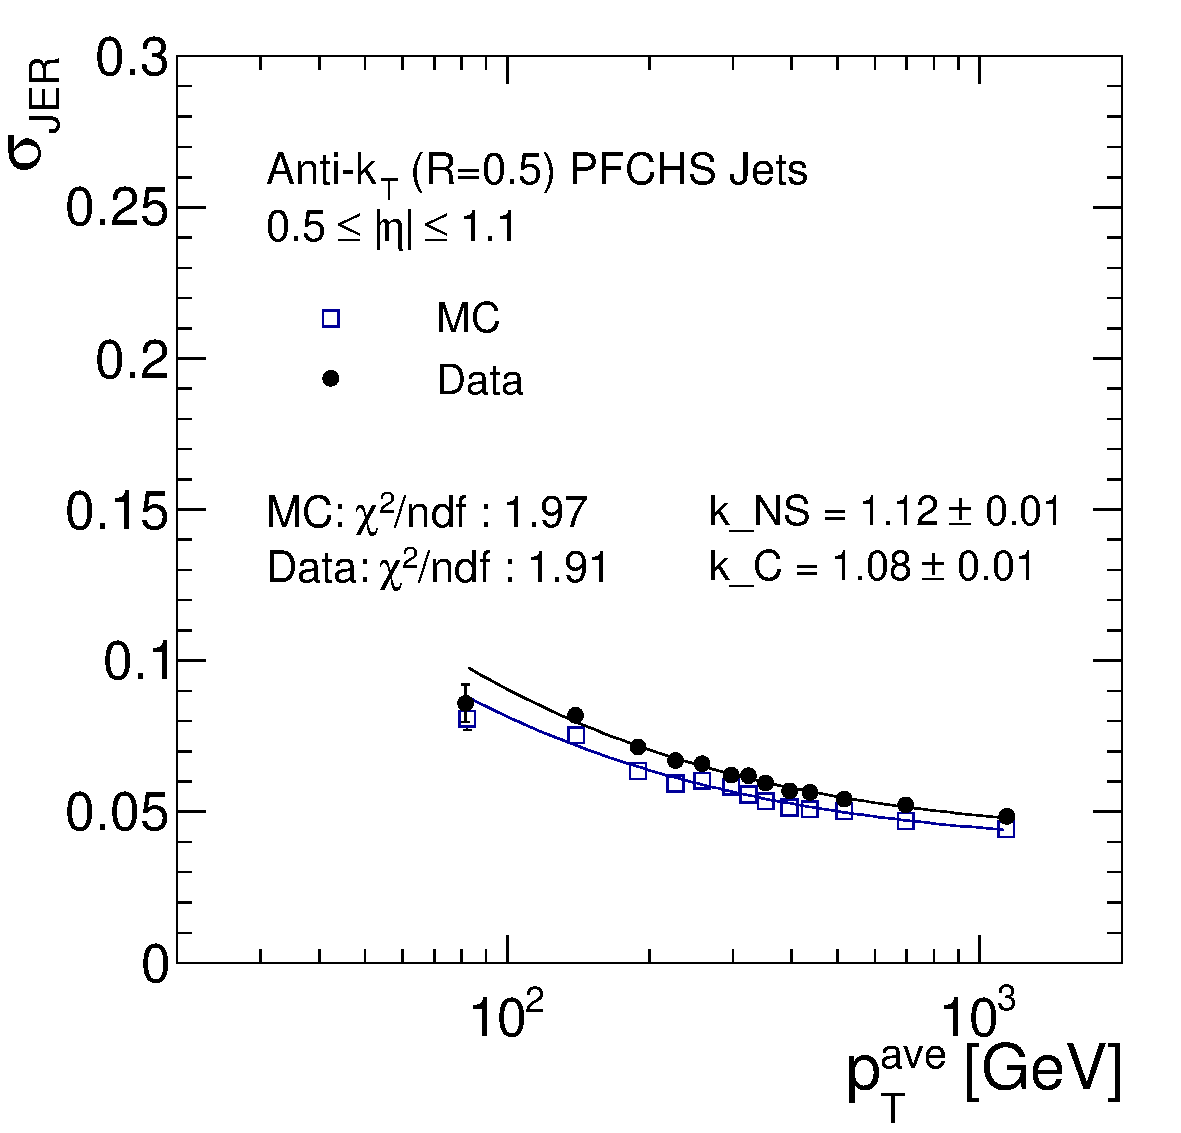
\includegraphics[width=0.49\textwidth]{figures/Pythia_NSCFit_Eta1_kNS_kC.pdf}\\
  \end{tabular}
  \caption{Results of fitting the resolution in data and simulation with the respective NSC-functions in the two central $|\eta|$ intervals.}
  \label{fig:NSC_Fits_3}
\end{figure} 
\begin{figure}[!p]
  \centering
  \begin{tabular}{cc}
                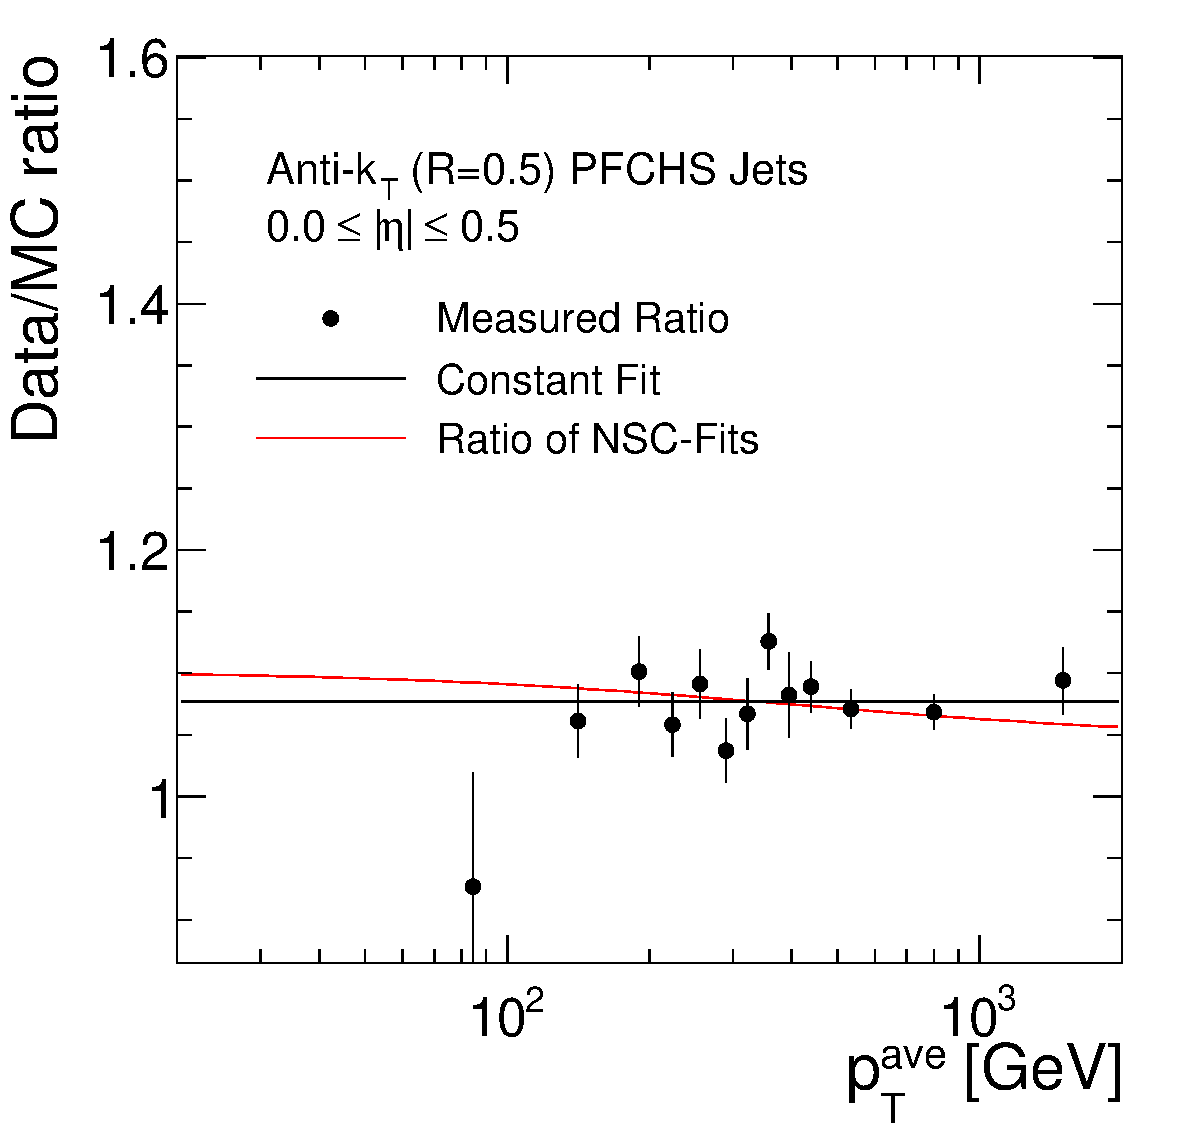
\includegraphics[width=0.49\textwidth]{figures/Pythia_NSCFit_Eta0_kNS_kC_ratio.pdf} &
                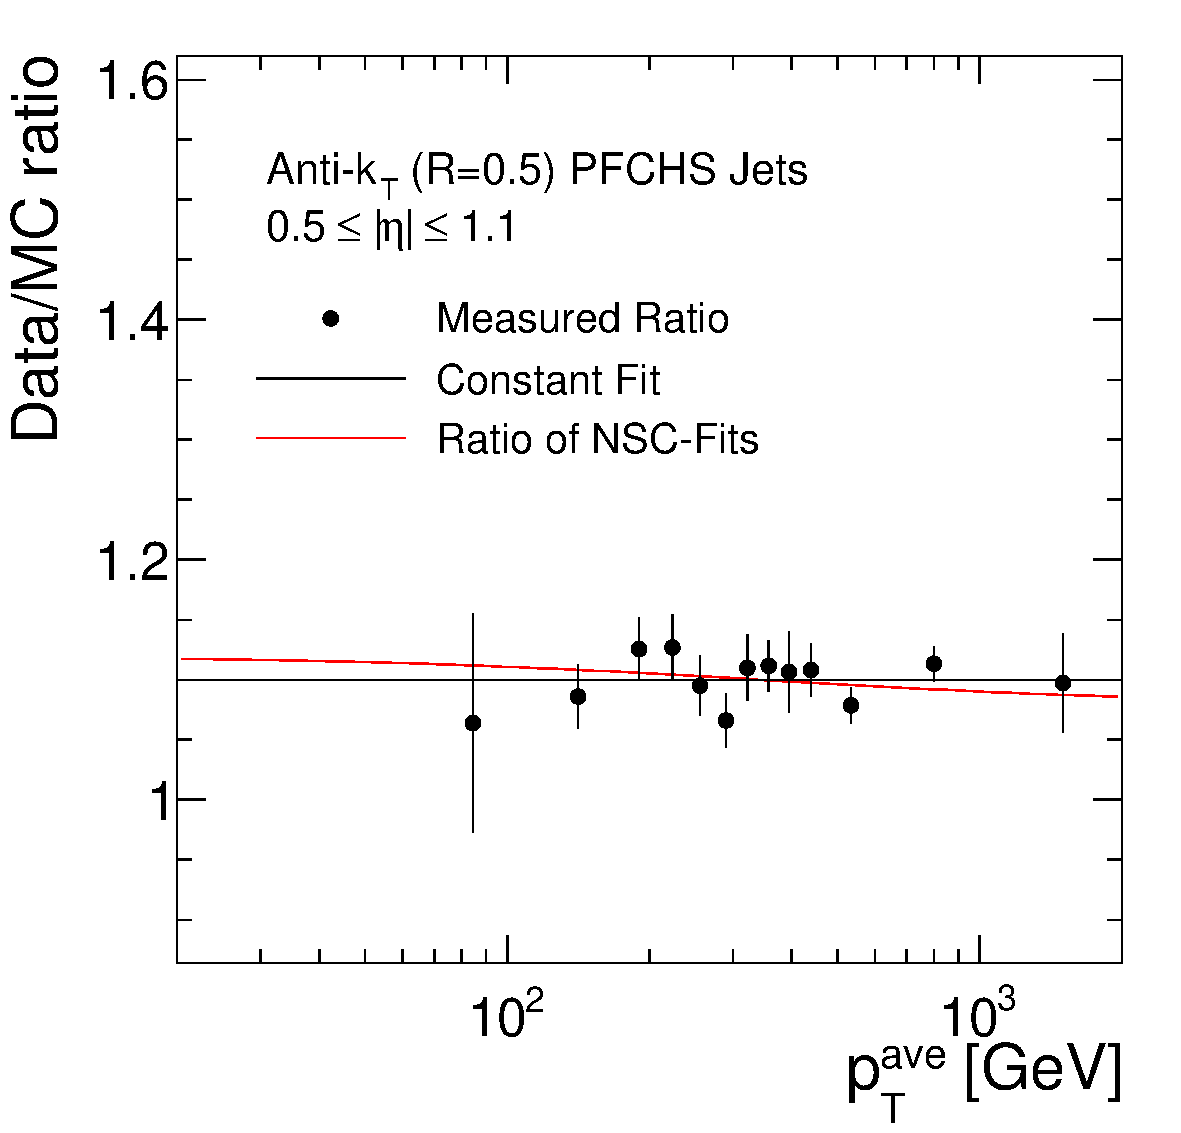
\includegraphics[width=0.49\textwidth]{figures/Pythia_NSCFit_Eta1_kNS_kC_ratio.pdf}\\
  \end{tabular}
  \caption{Ratio of the results fitting the resolution in data and simulation with the NSC-functions in the two central $|\eta|$ intervals together with the measured ratio and a constant fit.}
  \label{fig:NSC_Fits_ratio}
\end{figure} 

\item[Shape of the data-to-simulation ratio:] In general, the data-to-simulation ratio is determined by fitting the ratio of $\sigma^\mathrm{Data}_\mathrm{JER}$ to $\sigma^\mathrm{MC}_\mathrm{JER}$ with a constant. This assumes that the ratio is flat as a function of $\pt^\mathrm{ave}$. In order to test this assumption, one can fit the $\sigma^\mathrm{Data}_\mathrm{JER}$ and $\sigma^\mathrm{MC}_\mathrm{JER}$ distributions with a more model dependent approach. \\ 
The following function, denoted \textit{NSC-function}, is used to fit the resolution in simulation
\begin{equation}
f(\pt) = \sqrt{\frac{N^2}{\pt^{2}} + \frac{S^2}{\pt} + C^2}
\label{eq:NSC}
\end{equation}
with $\pt=\pt^\mathrm{ave}$ and the free parameters $N, S$ and $C$. This function is chosen in accordance to the parametrization typically used for the description of the relative energy-resolution in calorimeters (\cf Sec.~\ref{sec:cms}). If the resolution in simulation is fitted with this NSC-function, it is expected to find one common scale factor $k_{NSC}$ for the $N$, $S$ and $C$ parameters to describe the data, in case the data-to-simulation ratio is flat as a function of $\pt^\mathrm{ave}$. Significant differences between data and the actual modelling of the detector behaviour consequently can result in the necessity to use individual scale factors for the $k_N$, $k_S$ and $k_C$ parameters in order to describe the data from the fit results of the function to the simulation. \\
In order to test the assumption of a flat ratio, the data points are fitted with the following function 
\begin{equation}
f(\pt) = \sqrt{\frac{(k_{NS} \cdot N)^2}{\pt^{2}} + \frac{(k_{NS} \cdot S)^2}{\pt} + (k_{C} \cdot C)^2} 
\end{equation} 
with parameters $N, S$ and $C$ fixed to the fit results from simulation. This function makes use of one common scale factor for parameters $N$ and $S$ and another one for $C$. Since there are no events with low transverse momenta available, no sensitivity to the special characteristics of $N$ is expected and hence no separate scale factor for $N$ is defined. Furthermore, this means that this procedure can not be used to study influences from pileup. \\
Some example fits for the two most central $|\eta|$ intervals are summarized in Fig.~\ref{fig:NSC_Fits_3}. It turns out that typically the scale factors $k_{NS}$ and $k_{C}$ are not equal and thus a shape different from a constant could describe the measured data-to-simulation ratios as a function of \ptave as well. In order to illustrate how big this effect is, the ratio of the two fitted NSC-functions for data and simulation is shown together with the measured values and the constant fit in Fig.~\ref{fig:NSC_Fits_ratio}. It is visible that the ratio derived from the NSC-fits is also compatible with the measured values for the ratio. Consequently, a trend versus $\pt^\mathrm{ave}$ could be hidden in the measured points. The difference of the measured scale factors $k_{NS}$ and $k_{C}$ to the central value of the measurement from the constant fit amounts to about $2\%$ in the two central $|\eta|$ intervals. This is considered as systematic uncertainty for all $|\eta|$ intervals in order to compensate for this potentially hidden shape in the data-to-simulation ratio. Furthermore, this also covers possible differences of the scaling factors for jets with very low or very high transverse momenta which can not be directly measured in this analysis. Overall, this systematic uncertainty constitutes the major contribution to the total systematic uncertainty.
\end{description}
A summary of the data-to-simulation ratios measured with the dijet asymmetry method requiring that the two leading jets belong to the same $|\eta|$ interval together with all systematic uncertainties considered for the ratio is given in Tab.~\ref{tab:syst_uncert_summary}. Due to limited event numbers, no results could be determined for the two highest $|\eta|$ regions with this approach. In general, the measurement is limited by systematic effects which amount to uncertainties of about 2--2.5\% in the central detector part. However, in the $|\eta| \in [2.3, 2.8]$ region the measurement is limited by the statistical uncertainty.   

\begin{table}[!h]
\centering
\caption{Summary of the measured data-to-simulation ratios $c\mathrm{(Data/MC)}$ with absolute statistical uncertainty and systematic uncertainty for each uncertainty source in different $|\eta|$ regions up to $|\eta| = 2.8$.}
\label{tab:syst_uncert_summary}
 \makebox[\linewidth]{
\begin{tabular}{lcccccc}
\multicolumn{7}{c}{} \\
\toprule
 & & \multicolumn{5}{c}{$|\eta|$} \\
 & & 0.0--0.5 & 0.5--1.1 & 1.1--1.7 & 1.7--2.3 & 2.3--2.8  \\
 \midrule 
 $c\mathrm{(Data/MC)}$ & & 1.077 & 1.100 & 1.119 & 1.205 & 1.145  \\
 Stat. uncertainty & & $\pm$ 0.007 & $\pm$ 0.006 & $\pm$ 0.010 & $\pm$ 0.027 & $\pm$ 0.078  \\
\midrule
 PU & &  0.004 &  0.003 &  0.004 &  0.004 &  0.013   \\
 & & & & & & \\
 Particle-level imbalance & &  0.004 &  0.005 &  0.005 &  0.015 &  0.010  \\
 & & & & & & \\
 Jet energy scale & &  0.005 &  0.007 &  0.008 &  0.015 &  0.020  \\
 & & & & & & \\
 $\alpha$-spectrum & &  0.004 &  0.007 &  0.004 &  0.006 &  0.003  \\
 & & & & & & \\
 $\alpha$-range & &  0.005 &  0.009 &  0.004 &  0.011 &  0.012  \\
 & & & & & & \\
 Non-Gaussian tails & &  0.004 &  0.003 &  0.003 &  0.013 & 0.007  \\
 & & & & & & \\ 
 Jet Flavour & &  0.007 &  0.004 &  0.005 &  0.006 &  0.003  \\
 & & & & & & \\ 
 Ratio shape & &  0.022 &  0.022 &  0.022 &  0.024 &  0.023  \\
\midrule
 Total syst. uncertainty & & $\pm$ 0.025 & $\pm$ 0.027 & $\pm$ 0.026 & $\pm$ 0.038 & $\pm$ 0.038  \\
\bottomrule
\end{tabular}}
\end{table} 

\section{Extension of the Method to the Forward Detector Region}
\label{sec:jer_forward_extension}
The presented measurement with results summarized in Tab.~\ref{tab:syst_uncert_summary} is utilizing the dijet asymmetry method based on the requirement that the two leading jets in an event belong both to the same $|\eta|$ region. Consequently, the resolution of these two jets is equal which results in the simple relation expressed in Eq.~\ref{eq:asymmdef} between asymmetry width and jet resolution. However, the requirement that both leading jets have to belong to the same $|\eta|$ interval reduces significantly the available number of events. Especially in the forward region of the detector this is a problem, as the jets in these events have low transverse momenta and consequently have to be triggered by the lowest $\pt^\mathrm{ave}$ triggers which are highly prescaled. Hence, the available number of events is small and for the intervals $|\eta| > 2.8$ no data-to-simulation ratio could be determined with this approach. \\
In order to extend the analysis such that the data-to-simulation ratio can also be measured in the forward region of the detector, the requirement $i^{|\eta|}_{\mathrm{jet},1} = i^{|\eta|}_{\mathrm{jet},2}$ has to be dropped. Instead, events are selected in which the two leading jets belong to different pseudorapidity regions. Nonetheless, the jet resolution $\sigma (p_\mathrm{T}^{\mathrm{probe}})$ in a probe interval $|\eta_\mathrm{probe}|$ can be determined, if the resolution $\sigma (p_\mathrm{T}^{\mathrm{ref}})$ in a reference interval $|\eta_\mathrm{ref}|$ is known. \\
Based on Eq.~\ref{eq:asymm_first}, it can be shown that for $\langle p^\mathrm{probe}_\mathrm{T} \rangle = \langle p^\mathrm{ref}_\mathrm{T} \rangle = \langle \pt \rangle$ and $\sigma (p_\mathrm{T}^{\mathrm{probe}}) \neq \sigma (p_\mathrm{T}^{\mathrm{ref}})$ the relation
\begin{equation}
 \label{eq:asymm_forward}
  \frac{\sigma (p^\mathrm{probe}_\mathrm{T})}{\langle p_\mathrm{T} \rangle} = \sqrt{4 \cdot \sigma^{|\eta_{\mathrm{probe}|} \neq |\eta_{\mathrm{ref}}|}_{A} - \left(\frac{\sigma (p^\mathrm{ref}_\mathrm{T})}{\langle p_\mathrm{T} \rangle} \right)^2} 
 \end{equation}
is obtained. Here, $\sigma^{ |\eta_{\mathrm{probe}|} \neq |\eta_{\mathrm{ref}}|}_{A}$ is the width of the asymmetry calculated from the two leading jets in an event of which one jet belongs to a reference $|\eta|$ interval and the probe jet belongs to another $|\eta|$ region. The resolution of the jet in the reference interval has to be determined with the method imposing the same-$|\eta|$ requirement. The asymmetry width is meant to be corrected for additional jet activity and the particle-level imbalance determined from $\sigma^{|\eta_{\mathrm{probe}|} \neq |\eta_{\mathrm{ref}}|}_{A, \mathrm{gen}}$, \ie the asymmetry width of the generator asymmetry calculated for events in which the two leading jets do not belong to the same $|\eta|$ interval. The reference interval is preferred to be in the central detector region where the statistical precision from the same-$|\eta|$ measurement has already been sufficient. The statistical uncertainty of $\frac{\sigma (p^\mathrm{ref}_\mathrm{T})}{{\langle p_\mathrm{T} \rangle}}$ is propagated to the statistical uncertainty of $\frac{\sigma (p^\mathrm{probe}_\mathrm{T})}{\langle p_\mathrm{T} \rangle}$. \\
As long as both jets belong to the same $|\eta|$ region, residual effects from jet energy scale differences in data and simulation affect both jets the same way and should not have an impact on the resolution measurement. Since residual effects from the jet energy scale, where the mean of the asymmetry is shifted and not exactly located at zero, become more important, if both jets belong to different probe and reference intervals, a slightly modified definition of the asymmetry of
\begin{equation}
\label{eq:forwardasymmdef}
  \mathrm{A} = \frac{p^\mathrm{probe}_{\mathrm{T}} - p^\mathrm{ref}_{\mathrm{T}}}{p^\mathrm{probe}_{\mathrm{T}} + p^\mathrm{ref}_{\mathrm{T}}} 
 \end{equation}
is used for the reference-and-probe-interval measurement. The transverse momenta $p^\mathrm{ref}_{\mathrm{T}}$ and $p^\mathrm{probe}_{\mathrm{T}}$ correspond to the transverse momenta of the reference and probe jet, respectively. Accordingly, in the determination of the asymmetry width $\sigma_\mathrm{A}$ the mean of the distribution $A_\mathrm{mean}$ is also estimated. The asymmetry width is calculated as
\begin{equation}
\label{eq:forwardasymmwidthdef}
  \sigma_\mathrm{A} = \mathrm{RMS}_{98.5\%} = \sqrt{\frac{1}{y_i} \cdot \sum_{i}(A_i-A_\mathrm{mean})^2} 
 \end{equation}
with the frequency $y_i$ of the individual asymmetry values $A_i$. The sum over $i$ includes all values such that $98.5\%$ of the total asymmetry distribution are covered symmetric around the mean.\\
The measurement with the reference-and-probe-interval selection is performed taking the three innermost $|\eta|$ regions 0.0--0.5, 0.5--1.1 and 1.1--1.7 as reference intervals each. This allows a measurement of the data-to-simulation ratio also in the $|\eta|$ intervals 2.8--3.2 and 3.2--5.0. In addition, it provides for the innermost $|\eta|$ intervals an enhancement of the available number of events and thus a further reduction of the statistical uncertainties.\\
The systematic uncertainties of the two new measurements are evaluated according to same-$|\eta|$ measurement by varying a certain aspect in the determination of the data-to-simulation ratio and taking the absolute deviation from the nominal ratio as uncertainty. The variation is done simultaneously for the $\sigma^{ |\eta_{\mathrm{probe}|} \neq |\eta_{\mathrm{ref}}|}_{A}$ value as well as for $\frac{\sigma (p^\mathrm{ref}_\mathrm{T})}{{\langle p_\mathrm{T} \rangle}}$ for each uncertainty source. In general, the resulting uncertainties are of the same order as for the same-$|\eta|$ measurement. \\
A summary of the resulting data-to-simulation ratios determined in the measurements with the different reference intervals and the corresponding absolute statistical and total systematic uncertainties is shown in Tab.~\ref{tab:results_forward}. A detailed overview of these measurements, listing all individual components of systematic uncertainties, is given in App.~\ref{app:forward_results}. 
\begin{table}[!t]
\centering
\caption{Summary of the forward extension measurements with different reference intervals showing the nominal data-to-simulation ratios $c\mathrm{(Data/MC)}$ with absolute statistical and total systematic uncertainty in different probe $|\eta|$ regions.}
\label{tab:results_forward}
 \makebox[\linewidth]{
\begin{tabular}{cccccc}
\multicolumn{6}{c}{} \\
\toprule
 & & $|\eta_\mathrm{ref}| \in [0.0, 0.5]$ & $|\eta_\mathrm{ref}| \in [0.5, 1.1]$ & $|\eta_\mathrm{ref}| \in [1.1, 1.7]$ & \\
 $|\eta|$ & & $c\mathrm{(Data/MC)}$ $\pm \, \mathrm{stat.}$ $\pm \, \mathrm{syst.}$& $c\mathrm{(Data/MC)}$ $\pm \, \mathrm{stat.}$ $\pm \, \mathrm{syst.}$ & $c\mathrm{(Data/MC)}$ $\pm \, \mathrm{stat.}$ $\pm \, \mathrm{syst.}$ \\
\midrule
 $0.0 - 0.5$ & & -----                               &  1.081 $\pm \, 0.008$ $\pm \, 0.026$ & 1.084 $\pm \, 0.012$ $\pm \, 0.033$ \\
 & & & & & \\
 $0.5 - 1.1$ & & 1.106 $\pm \, 0.008$ $\pm \, 0.028$ &  -----                              & 1.082 $\pm \, 0.012$ $\pm \, 0.036$ \\
 & & & & & \\
 $1.1 - 1.7$ & & 1.133 $\pm \, 0.009$ $\pm \, 0.030$ & 1.111 $\pm \, 0.009$ $\pm \, 0.030$ &  -----               \\
 & & & & & \\
 $1.7 - 2.3$ & & 1.227 $\pm \, 0.025$ $\pm \, 0.058$ & 1.206 $\pm \, 0.023$ $\pm \, 0.039$ & 1.189 $\pm \, 0.031$ $\pm \, 0.063$ \\
 & & & & & \\
 $2.3 - 2.8$ & & 1.253 $\pm \, 0.047$ $\pm \, 0.112$ & 1.300 $\pm \, 0.047$ $\pm \, 0.082$ & 1.250 $\pm \, 0.051$ $\pm \, 0.065$ \\
 & & & & & \\
 $2.8 - 3.2$ & & 1.410 $\pm \, 0.068$ $\pm \, 0.067$ & 1.356 $\pm \, 0.058$ $\pm \, 0.105$ & 1.432 $\pm \, 0.066$ $\pm \, 0.077$ \\
 & & & & & \\
 $3.2 - 5.0$ & & 1.171 $\pm \, 0.116$ $\pm \, 0.079$ & 0.829 $\pm \, 0.082$ $\pm \, 0.149$ & 1.137 $\pm \, 0.105$ $\pm \, 0.096$ \\
\bottomrule
\end{tabular}}
\end{table} 

\section{Measurement for Simulated Events Obtained with the \herwig Generator} 
\label{sec:jer_result_herwig}
The data-to-simulation ratio has been determined with respect to simulated events obtained from the \pythia generator. However, other generators use for instance different fragmentation models. Thus, it is interesting to study, if the determined data-to-simulation ratio is generator independent. For this study, the data-to-simulation ratio is derived for simulated events not taken from the \pythia generator, but for events obtained from \herwig tune EE3C. This is the same sample as introduced in Sec.~\ref{sec:jer_syst_unc} for the evaluation of the systematic PLI uncertainty. \\
The measurement is performed applying the same selection criteria, as described in Sec.~\ref{subsec:jer_sel_cuts}. Also the pileup reweighting procedure is performed as described there. In Fig.~\ref{fig:control_plots_herwig}, the inclusive $\pt^\mathrm{ave}$ spectrum is compared in data and simulation for simulated events taken from \herwig. The agreement of the \ptave spectrum between data and simulation looks reasonable and exhibits a similar trend as the spectrum in simulated events from \pythia.\\
The nominal values of the data-to-simulation ratio have been determined with statistical uncertainties with the same-$|\eta|$ requirement as well as for the three different reference-and-probe jet combinations. Since this study is only used as cross-check, no systematic uncertainties have been studied. The resulting data-to-simulation ratios for simulated events taken from \herwig together with statistical uncertainties for the different measurements are summarized in Tab.~\ref{tab:result_herwig}. \\
In general, the obtained data-to-simulation ratios for \herwig agree among each other and are quite similar to the values obtained from \pythia for most $|\eta|$ regions. Some further discussion follows in Sec.~\ref{subsec:jer_combination}.
\begin{figure}[!p]
  \centering
  \begin{tabular}{c}
                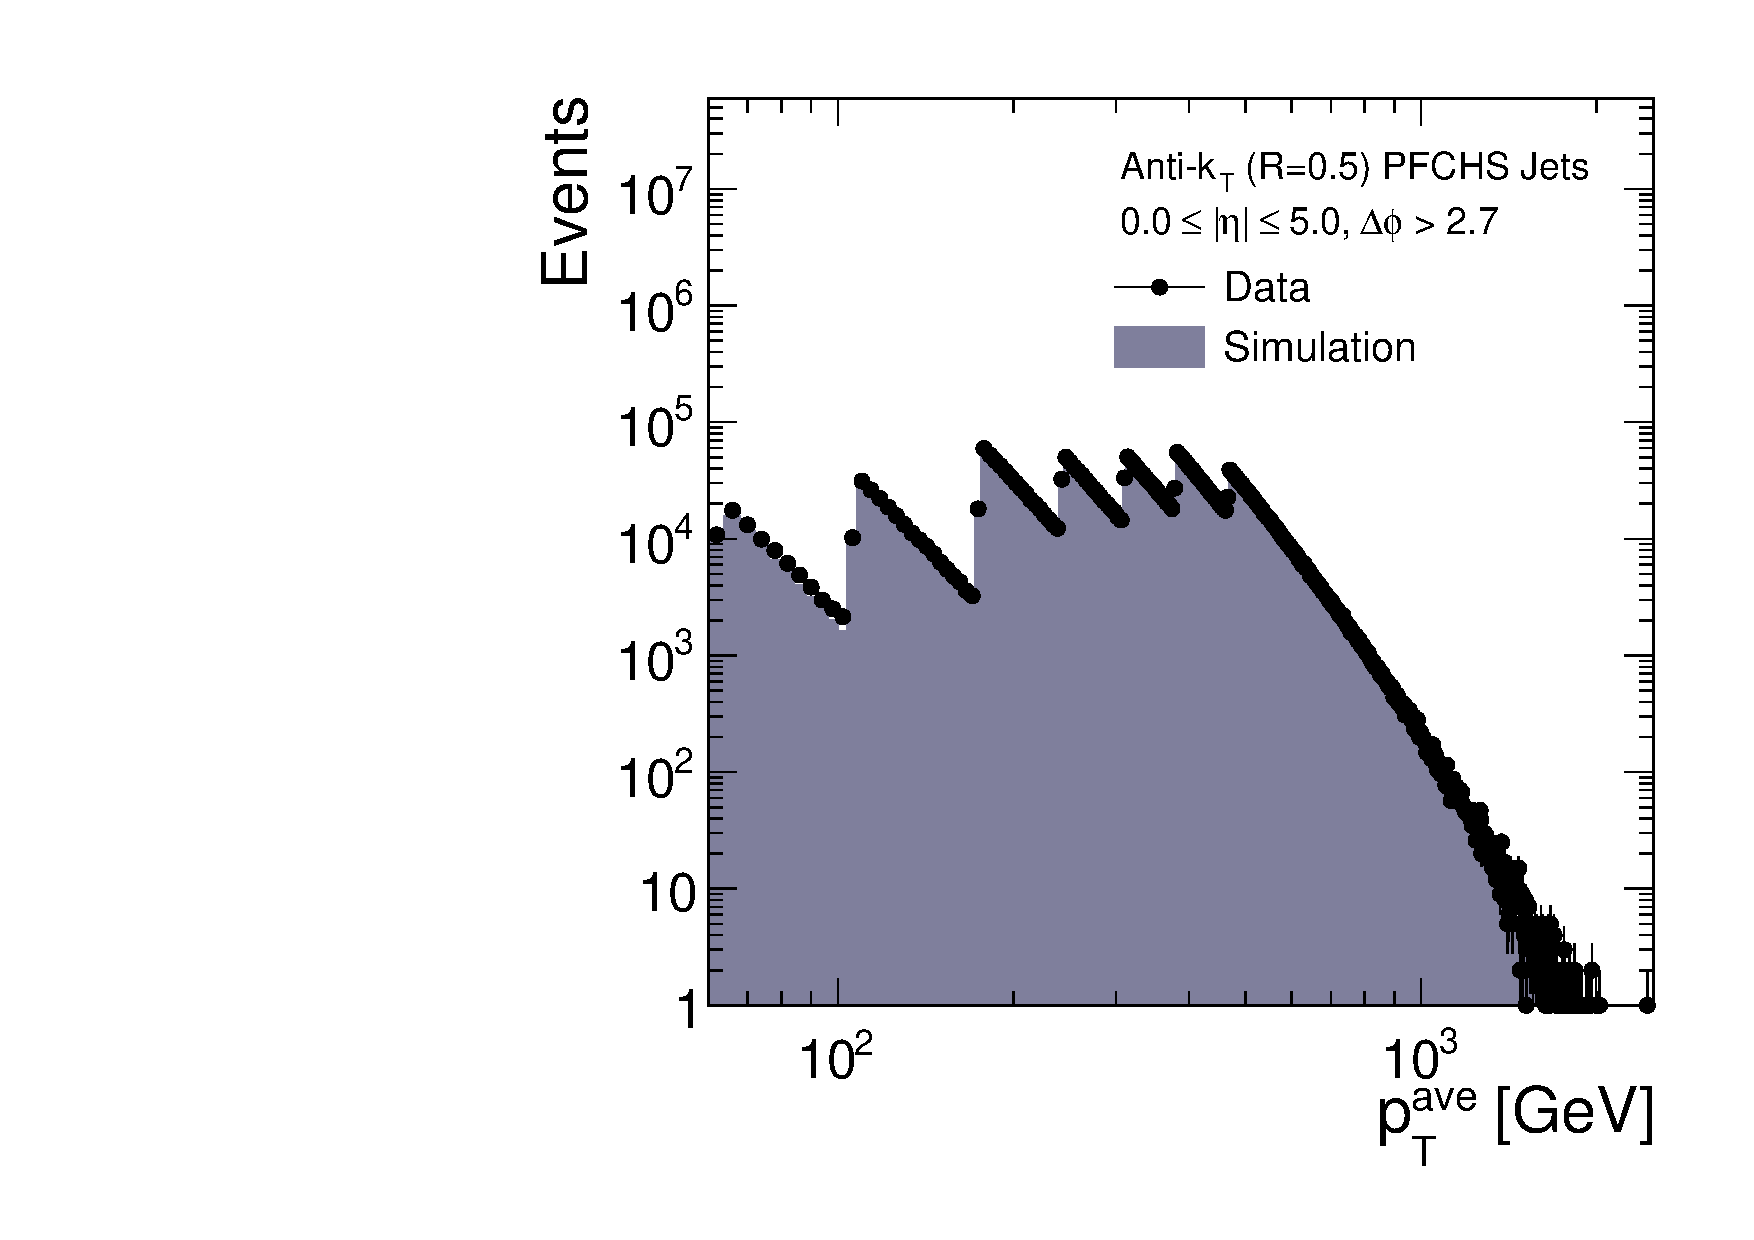
\includegraphics[width=0.49\textwidth]{figures/HerwigPtAve__AfterAsymmHistos.pdf}
  \end{tabular}
  \caption{Inclusive $\pt^\mathrm{ave}$ spectrum of events after the event selection in data and in simulated events generated with \herwig.}
  \label{fig:control_plots_herwig}
\end{figure}
\begin{table}[!p]
\centering
\caption{Measured data-to-simulation ratio in various probe $|\eta|$ regions with statistical uncertainty for simulated events obtained with the \herwig generator.}
\label{tab:result_herwig}
 \makebox[\linewidth]{
\begin{tabular}{ccccccc}
\multicolumn{7}{c}{} \\
\toprule
 & & $|\eta_{1}|$ = $|\eta_{2}|$ & $|\eta_\mathrm{ref}| \in [0.0, 0.5]$ & $|\eta_\mathrm{ref}| \in [0.5, 1.1]$ & $|\eta_\mathrm{ref}| \in [1.1, 1.7]$ & \\
 $|\eta|$ & & $c\mathrm{(Data/MC)}$ & $c\mathrm{(Data/MC)}$ & $c\mathrm{(Data/MC)}$ & $c\mathrm{(Data/MC)}$ \\
\midrule
 $0.0 - 0.5$ & & 1.090 $\pm \, 0.008$ & -----                &  1.091 $\pm \, 0.011$ & 1.129 $\pm \, 0.017$ \\
 & & & & & &\\
 $0.5 - 1.1$ & & 1.107 $\pm \, 0.008$ & 1.111 $\pm \, 0.010$ &  -----                & 1.121 $\pm \, 0.016$ \\
 & & & & & &\\
 $1.1 - 1.7$ & & 1.117 $\pm \, 0.013$ & 1.177 $\pm \, 0.013$ & 1.149 $\pm \, 0.012$  &  -----               \\
 & & & & & &\\
 $1.7 - 2.3$ & & 1.297 $\pm \, 0.038$ & 1.212 $\pm \, 0.035$ & 1.229 $\pm \, 0.033$  & 1.187 $\pm \, 0.041$ \\
 & & & & & &\\
 $2.3 - 2.8$ & & 1.085 $\pm \, 0.080$ & 1.231 $\pm \, 0.072$ & 1.178 $\pm \, 0.061$  & 1.363 $\pm \, 0.087$ \\
 & & & & & &\\
 $2.8 - 3.2$ & &  -----               & 1.368 $\pm \, 0.094$ & 1.259 $\pm \, 0.061$  & 1.488 $\pm \, 0.112$ \\
 & & & & & &\\
 $3.2 - 5.0$ & &  -----               & 1.245 $\pm \, 0.158$ & 1.124 $\pm \, 0.128$  & 1.324 $\pm \, 0.215$ \\
\bottomrule
\end{tabular}}
\end{table} 

\section{Results}
\label{sec:jer_results}

\subsection{Determination of a combined result}
\label{subsec:jer_combination}
\begin{table}[!t]
\centering
\caption{Measured data-to-simulation ratio in various $|\eta|$ regions with statistical and systematic uncertainty as well as the total uncertainty.}
\label{tab:result}
\makebox[\linewidth]{
\begin{tabular}{ccc|cc|cc}
\multicolumn{7}{c}{} \\
\toprule
 $|\eta|$ & & $c\mathrm{(Data/MC)}$ & $\rm{stat.}$ & $\rm{syst.}$ & $\rm{tot.}$\\
\midrule
 $0.0 - 0.5$ & & 1.079 & $\pm \, 0.005$ & $\pm \, 0.026$ & $\pm \, 0.026$ \\
 & & & & & &\\
 $0.5 - 1.1$ & & 1.099 & $\pm \, 0.005$ & $\pm \, 0.028$ & $\pm \, 0.028$ \\
 & & & & & &\\
 $1.1 - 1.7$ & & 1.121 & $\pm \, 0.005$ & $\pm \, 0.029$ & $\pm \, 0.029$ \\
 & & & & & &\\
 $1.7 - 2.3$ & & 1.208 & $\pm \, 0.013$ & $\pm \, 0.045$ & $\pm \, 0.046$ \\
 & & & & & &\\
 $2.3 - 2.8$ & & 1.254 & $\pm \, 0.026$ & $\pm \, 0.056$ & $\pm \, 0.062$ \\
 & & & & & &\\
 $2.8 - 3.2$ & & 1.395 & $\pm \, 0.036$ & $\pm \, 0.051$ & $\pm \, 0.063$ \\
 & & & & & &\\
 $3.2 - 5.0$ & & 1.056 & $\pm \, 0.048$ & $\pm \, 0.185$ & $\pm \, 0.191$ \\
\bottomrule
\end{tabular}}
\end{table} 
The data-to-simulation ratio has been measured with different approaches for various $|\eta|$ regions. Since these are in general in good agreement, the results obtained from the individual measurements are combined into one single scale factor for each $|\eta|$ region. This combination is for all $|\eta|$ regions -- except for the very last $|\eta|$ region ranging from 3.2--5.0 which is discussed separately -- derived from the measurements done with simulated events from \pythia while the \herwig results are only used as cross check. \\
The combined data-to-simulation ratios are calculated as weighted mean from the individual measurements with the same-$|\eta|$ requirement and the three central-forward combinations. Each measurement is weighted by its statistical uncertainty. For the evaluation of the systematic uncertainties for the combined result the systematic shift of the weighted mean caused by the systematic shifts of the single measurements is determined. This means that for each uncertainty source the individual up and down shifts to the nominal ratio of each measurement are taken and combined as the weighted mean using the statistical uncertainty just as for the nominal mean. Consequently, the difference of each systematically shifted weighted mean to the nominal weighted mean is the respective systematic uncertainty for the combination. \\
The $|\eta|$ region covering the most forward region of the detector from 3.2--5.0, \ie the hadronic forward, behaves a bit special compared to the others. In contrast to the other $|\eta|$ regions, the individual measurements from \pythia and \herwig have a very large spread of ratios from 0.83 up to 1.32 in this particular interval. If those are combined for this interval, it is in this case reasonable to use all six individual measurements from \pythia as well as from \herwig to find a result which covers all of these partly very different ratios. If the combination is done following the same procedure as described for the other intervals considering all nominal values obtained with \pythia and \herwig while taking the systematic uncertainty from the combined \pythia results, the total scale factor would be 1.056 $\pm$ 0.048 ($\mathrm{stat.\; unc.}$) $\pm$ 0.079 ($\mathrm{syst. \; unc.}$) (= 0.092 total unc.). In order to test the consistency of this combined value with the single measurements the $\chi^2/\mathrm{ndf}$ is calculated. This results in $\chi^2/\mathrm{ndf} = 4.3$. This shows that the obtained total uncertainty is too small to reasonably cover all individual results. Hence, the systematic uncertainty is increased to a value of $\pm$ 0.185 which gives a total uncertainty of $\pm$ 0.191 and results in a $\chi^2/\mathrm{ndf} = 1.0$, such that the single measurements are well represented by this combined result and the indivudal shifts are covered by the assigned uncertainty.\\
The obtained data-to-simulation ratios for the various $|\eta|$ regions are summarized in Tab.~\ref{tab:result}, together with the statistical and systematic uncertainties. In addition, Fig.~\ref{fig:result_2012} shows the measured ratios together with the total uncertainty. This is given by the quadratic sum of the statistical and systematic uncertainties. \\
The determined ratios vary from 1.06 to 1.40 and exceed the value of one in all detector parts. Possible sources of this difference can be, \eg mismodelled noise effects or inhomogenities of the detector. However, no distinct reason for the discrepancy of the resolution in data and simulation has been identified yet. 

\begin{figure}[!t]
  \centering
  \begin{tabular}{c}
                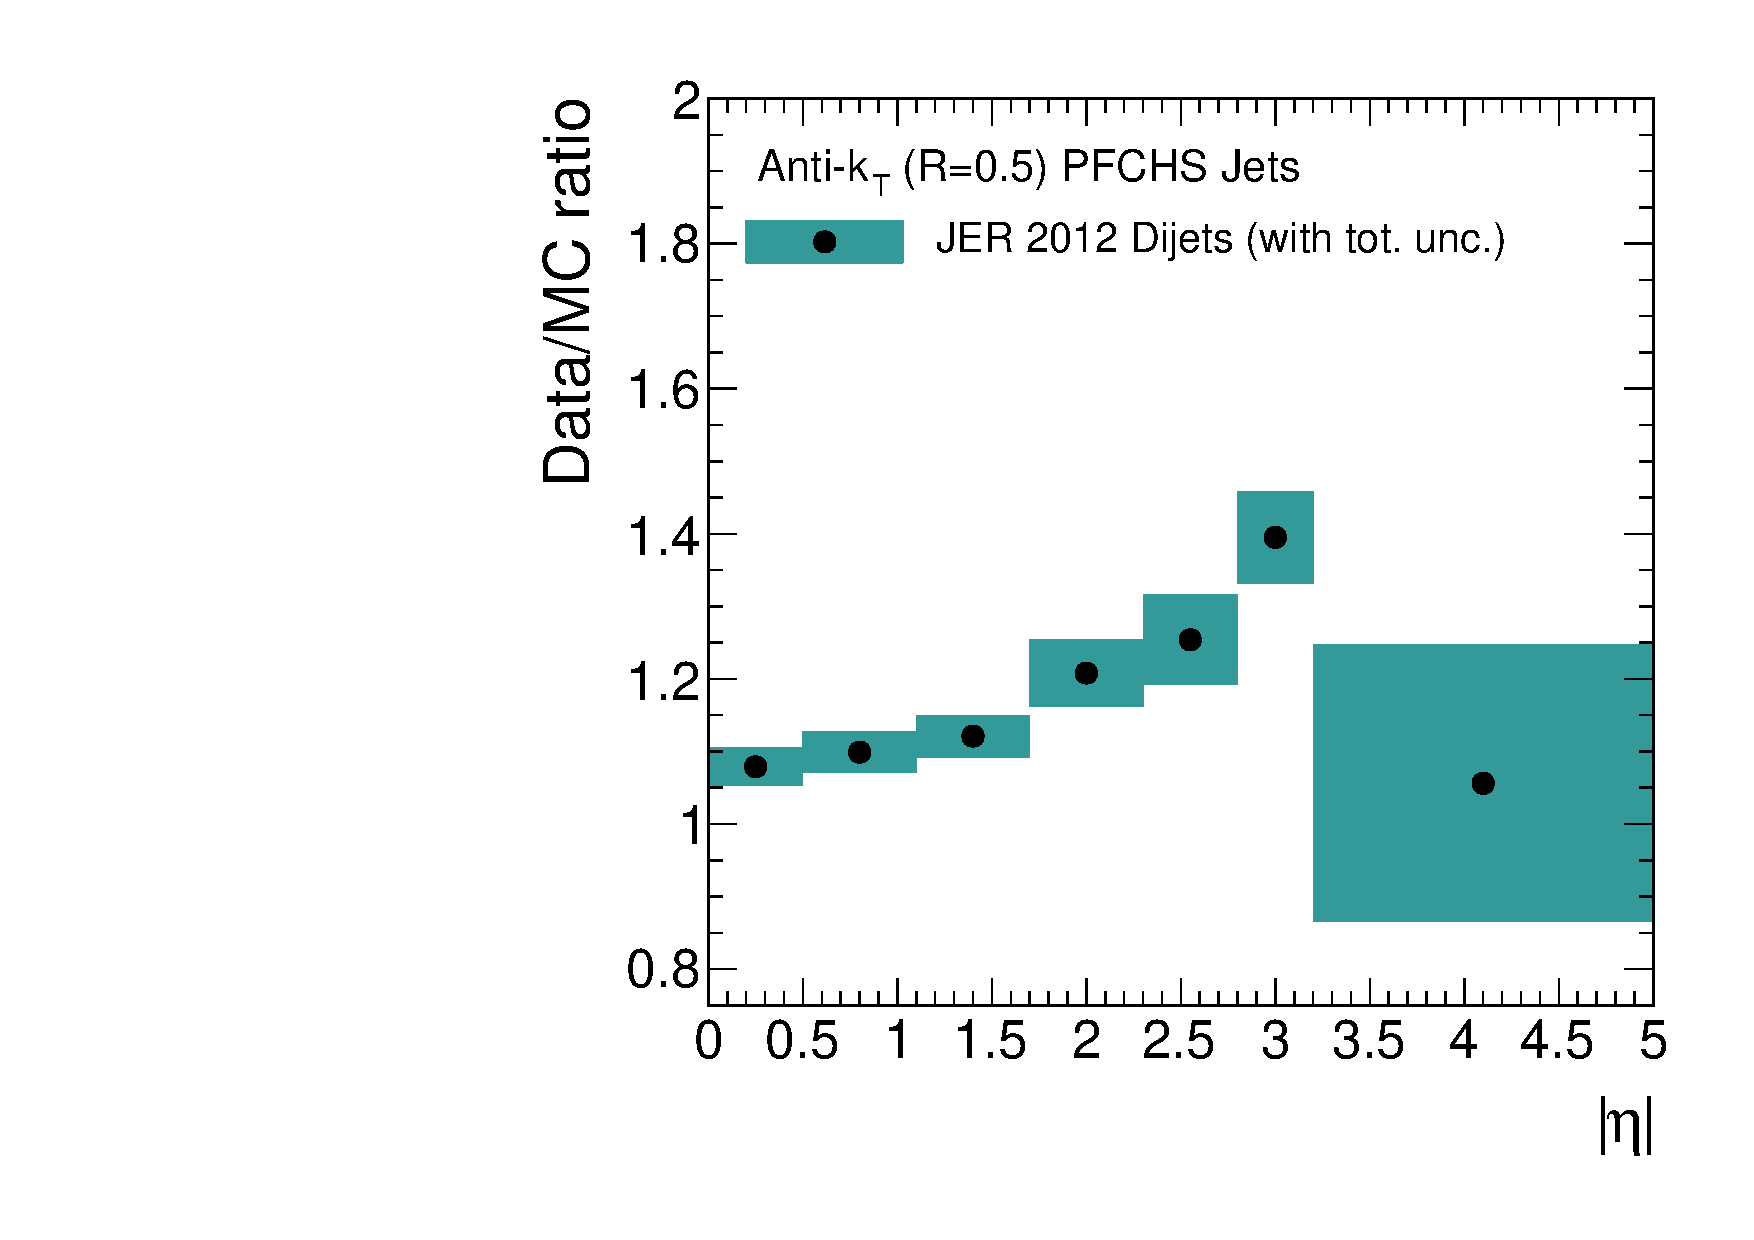
\includegraphics[width=0.6\textwidth]{figures/JER_2012_final_combination_v1.pdf}
  \end{tabular}
  \caption{Measured data-to-simulation ratio in various $|\eta|$ regions displayed with total uncertainty.}
  \label{fig:result_2012}
\end{figure}
 
\subsection{Comparison to Other Measurements}
\label{subsec:jer_results_comparison}
Earlier analyses using dijet events for data collected at $\sqrt{s}=7$\tev have obtained similar results showing data-to-simulation ratios greater than one. A complementary approach is followed using $\gamma +\rm{jet}$ events which offer a very precise opportunity to measure the jet resolution due to the excellent resolution of the photon energy. A comparison of the numbers derived in the context of this thesis to the latest results from dijet events obtained at $\sqrt{s}=7$\tev~\cite{thesis:Schroeder} and results for $\gamma +\rm{jet}$ measurements at $\sqrt{s}=8$\tev~\cite{CMS-AN-2013-179} are shown together in Fig.~\ref{fig:result_comparison}.
\begin{figure}[!t]
  \centering
  \begin{tabular}{cc}
                \includegraphics[width=0.49\textwidth]{figures/JER_2012_compPhoton_final_combination_v1.pdf} &
                \includegraphics[width=0.49\textwidth]{figures/JER_2012_comp2011_final_combination_v1.pdf}
  \end{tabular}
  \caption{Measured data-to-simulation ratio in various $|\eta|$ regions displayed with total uncertainty. Comparison to results obtained for $\sqrt{s}=8$\tev data from $\gamma +\rm{jet}$ events $(\textit{left})$ and to $\sqrt{s}=7$\tev data from dijet events $(\textit{right})$.}
  \label{fig:result_comparison}
\end{figure}
\\
The results obtained from different methods and for the different centre of mass energies are well compatible with each other. The main advantage of the dijet measurement presented in this thesis compared to the $\gamma +\rm{jet}$ analysis is that one obtains also results for the outermost $|\eta|$ region. In addition, the total uncertainties in the other $|\eta|$ regions are at a same accuracy or even slightly lower. \\
In comparison to the $\sqrt{s}=7$\tev results from dijet events, the total uncertainty could be significantly reduced by incorporating the correlation among the different inclusive $\alpha$ regions in the extrapolation procedure. In the previous analyses, the statistical uncertainties were underestimated by not considering the above mentioned correlation. This effect was compensated by introducing a rather conservative systematic uncertainty on the extrapolation to zero additional jet activity. Since the treatment of the statistical uncertainty has been changed in this analysis, the estimation of systematic effects could be adjusted accordingly and lead to the overall reduced uncertainty values summarized in Table~\ref{tab:result}.

\subsection{Impact of the Improved JER Measurement}
\label{subsec:jer_results_impact}
As mentioned in the introduction of this chapter, the jet transverse-momentum resolution is a key ingredient for several analyses. In this section, the impact of the improved JER measurement is discussed for two use cases. \\
First, the influence of the JER measurement on the jet energy corrections is examined. As the derived data-to-simulation factors for the resolution feature a dependence on $|\eta|$ and denote difference data and simulation, it is important to propagate their uncertainty to the L2 residual correction of the jet energy scale. The impact of the JER uncertainty on the L2 residual correction is illustrated in Fig.~\ref{fig:result_jec_impact}.  
\begin{figure}[!h]
  \centering
  \begin{tabular}{c}
                \includegraphics[width=0.49\textwidth]{figures/newJER_L2V4_L3fixed-ratio_mod.jpg} 
  \end{tabular}
  \caption{Impact of the JER uncertainty on the L2 residual correction. The variation of the correction with respect to the nominal correction factor is shown as a function of the pseudorapidity~\cite{DRathjens}. For further explanation see text.}
  \label{fig:result_jec_impact}
\end{figure}
\\
The blue-shaded band denotes the uncertainty on the L2 residual correction caused by the uncertainty of the JER measurement from 2011 dijet data, as illustrated in Fig.~\ref{fig:result_comparison} (right). Red and green dots illustrate the resulting up and down variation of the L2 residual correction when propagating the JER uncertainty, as determined in the analysis presented in this thesis. Closed and open symbols represent two different methods used to derive the L2 residual correction. Especially in the forward region of the detector, the uncertainty is reduced by about 50\%. \\
Furthermore, the improved jet resolution measurement has a major impact on the determination of the top-quark mass. The currently most precise single measurement of the top-quark mass from CMS is performed in the lepton+jets channel and yields a top quark mass of $m_t = 172.04 \pm 0.19\; \mathrm{(stat.+JSF)} \pm 0.75\;\mathrm{(syst.)}$\gev~\cite{CMS-PAS-TOP-14-001}. The propagated uncertainty of the jet transverse-momentum resolution is among the dominant systematic uncertainties and amounts to 0.26\gev when considering the data-to-simulation scale factors as measured with the 2011 dijet data. The improved uncertainty on the JER scale factors decreases the contribution to the systematic uncertainties of the top-quark mass measurement from 0.26\gev to 0.11\gev. Accordingly, the total systematic uncertainty drops from 0.75\gev to 0.71\gev~\cite{MSeidel}. Consequently, the precision of the top-quark mass measurement in the above mentioned lepton+jets channel reaches the accuracy of the currently overall most precise single measurement of the top-quark mass which yields a total uncertainty of 0.76\gev, as performed by the \dzero experiment~\cite{Abazov:2014dpa}.   

\section{Adjustment of the MC-Resolution to Data}
\label{sec:jer_adjustment}
The determined data-to-simulation ratios as given in Tab.~\ref{fig:result_2012} can be used to adjust the resolution in simulated events to match the measured resolution in data. This can be done with different approaches depending on what the actual purpose of the analysis is. \\
If a correspondence of the resolution in data and simulation per jet is needed (as it was used in Sec.~\ref{sec:jer_validation_ratio}), each detector-level jet in the simulation can be scaled according to the momentum difference to the respective generator-level jet. Since the resolution is proportional to this momentum difference, an adjustment of the resolution to data corresponds to scaling the momentum difference by the measured scale factor as expressed already in Eq.~\ref{eq:smear_gen}. \\
Alternatively, the resolution in simulation can be adjusted by convolution with a Gaussian. Taking a Gaussian function with appropiate width $\sigma_{c}$, the width of the response function after convolution corresponds to the resolution in data according to 
\begin{equation}
\sigma_{c} = \sqrt{c^2-1} \cdot \left( \frac{\sigma_{MC}}{\pt} \right) \; .
\label{eq:res_adjust}
\end{equation}
Consequently, this method can only be used, if $c > 1$. \\
Further discussion about the adjustment of the resolution in simulation to data can be found in Section~\ref{subsec:RA2_QCD} where this is actually applied in the estimation of background contributions arising from QCD multijet events to a search for new physics in an all-jet final state.  

%\section{Impact of the Resolution Measurement on Other Analyses}
%\label{sec:jer_impact}












